\def\topic{Chapter: Logic}%Foundations of mathematics
\ifdefined\MyHeaderIncluded
\else
\def\qwertyflag{true}

\ifdefined\MyHeaderIncluded

\else
  \newcommand{\foobar}{FooBar}
  \def\MyHeaderIncluded{true}
% if is till the end of the file

\documentclass[10pt,a4paper]{article}
\usepackage[utf8]{inputenc}
%\usepackage[german]{babel}
%\usepackage[cyrillic]{babel}
\usepackage[T1]{fontenc}
%\usepackage[T2A]{fontenc}
%\usepackage[english, russian]{babel}
\usepackage{amsmath}
\usepackage{amsfonts}
\usepackage{amssymb}
\usepackage{amsthm}
\usepackage{mathtools} %coloneqq

\usepackage{bussproofs} %

%\renewcommand{\thesubsection}{\arabic{subsection}}
%\newtheorem{thm}{Theorem}[section]
%\renewcommand{\thethm}{\arabic{subsection}.\arabic{thm}}

\usepackage{thmtools}
\usepackage{hyperref}
\hypersetup{
    colorlinks=true,
    linkcolor=blue,
    filecolor=magenta,      
    urlcolor=cyan,
    pdftitle={Overleaf Example},
    %pdfpagemode=FullScreen,
    }
%\usepackage{stix-type1}%\turnediota
\theoremstyle{definition}

\newtheorem{constructor}{Constructor}[section]
\newtheorem{iaxiom}{Axiom}
\newtheorem{axiom}{Axiom}
\newtheorem*{axiom*}{Axiom}
\newtheorem{definition}{Definition}[section]
\newtheorem*{definition*}{Definition}
\newtheorem{remark}{Remark}[section]
\newtheorem*{remark*}{Remark}
\newtheorem{recall}{Recall}[section]
\newtheorem*{recall*}{Recall}

\newtheorem{lemma}{Lemma}[section]
\newtheorem{theorem}{Theorem}[section]
\newtheorem*{theorem*}{Theorem}
\newtheorem{note}{Note}[section]
\usepackage{etoolbox}

%\newcommand*{\@Dashv}[2]{%
%  \reflectbox{$\m@th#1#2$}%
%}
\newcommand*{\separation}[3]{% 1)binder, 2)set, 3)condition
  \{#1\in #2: #3\}
}

% https://www.freecodecamp.org/news/simple-regex-tricks-for-beginners-3acb3fa257cb/
%  \\mathcal\{T\} |---> \topology
%  \\mathcal\{([^\}]*)\}   |--->  $1
\newcommand{\AND}{\ \ \&\ \ }
\newcommand{\any}{\mathrm{\ any}}
\newcommand{\borel}{\mathcal{B}}
\newcommand{\can}{\mathrm{can}}
\newcommand{\canonize}{\mathrm{canonize}}
\newcommand{\closure}{\mbox{cl}}
\newcommand{\complex}{\mathbb{C}}
\newcommand{\converges}{\longrightarrow}
\newcommand{\countable}{\mbox{\ countable}}
\newcommand{\ldefined}{\mbox{\ defined}}
\newcommand{\dom}{\mbox{dom}}
\newcommand{\Dom}{\mbox{Dom}}
\newcommand{\Done}{\noindent \textbf{Done.}\\}
\newcommand{\lexists}{\mbox{\ exists}}
\newcommand{\lforall}{\mbox{\ forall}}
\newcommand{\lunique}{\mbox{\ unique}}
\newcommand{\family}{\mathrm{\ family}}
\newcommand{\Fm}{\mathrm{Fm}}
\newcommand{\FuncSymb}{\mathrm{FuncSymb}}
\newcommand{\function}{\mathrm{\ function}}
\newcommand{\functional}{\mbox{\ functional}}
\newcommand{\IFF}{\ \Longleftrightarrow\ }
\renewcommand{\iff}{\ \longleftrightarrow\ }
\newcommand{\IMPLIES}{\ \Longrightarrow\ }
\renewcommand{\implies}{\ \longrightarrow\ }
\newcommand{\Inf}{\mathrm{Inf}}
\newcommand{\injective}{\mbox{\ injective}}
\newcommand{\injection}{\mbox{\ injection}}
\newcommand{\interior}{\mbox{int}}
\newcommand{\intersection}{\bigcap}
\newcommand{\isempty}{\mathrm{\ empty}}
\newcommand{\LB}{\mathrm{LB}}
\newcommand{\nghbset}{\mathcal{N}}
\newcommand{\nonempty}{\mathrm{\ nonempty}}
\newcommand{\Ord}{\mathrm{Ord}}
\newcommand{\power}{\mathcal{P}}
\newcommand{\pr}{\mathrm{pr}}
\newcommand{\fst}{\mathrm{fst}}
\newcommand{\snd}{\mathrm{snd}}
\newcommand{\PredSymb}{\mathrm{PredSymb}}
\newcommand{\Proof}{\noindent \textbf{Proof.}\\}
\newcommand{\ran}{\mathrm{ran}}
\newcommand{\Ran}{\mathrm{Ran}}
\newcommand{\real}{\mathbb{R}}
\newcommand{\relation}{\mathrm{\ relation}}
\newcommand{\set}{\mathrm{\ set}}
\newcommand{\singleton}{\mathrm{\ singleton}}
\newcommand{\semantics}{\mathrm{semantics}}
\newcommand{\semialgebra}{\mathcal{S}}
\newcommand{\Sup}{\mathrm{Sup}}
\newcommand{\surjective}{\mbox{\ surjective\ on\ }}
\newcommand{\Term}{\mathrm{Term}}
\newcommand{\Type}{\mathrm{Type}}
\newcommand{\topology}{\mathcal{T}}
\newcommand{\total}{\mbox{\ total\ on\ }}
\newcommand{\transitive}{\mathrm{\ transitive}}
\newcommand{\union}{\bigcup}
\newcommand{\lTrue}{\mathrm{True}}
\newcommand{\lFalse}{\mathrm{False}}
\newcommand{\lUncertain}{\mathrm{Uncertain}}
\newcommand{\lif}{\mathrm{if}}
\newcommand{\lthen}{\mathrm{then}}
\newcommand{\lelse}{\mathrm{else}}
\newcommand{\lexception}{\mathrm{exception}}
\newcommand{\lundef}{\mathrm{undef}}
\newcommand{\univocal}{\mathrm{\ univocal}}
\newcommand{\univocalat}{\mathrm{\ univocal\ at\ }}
\newcommand{\UB}{\mathrm{UB}}
\newcommand{\Un}{\mathcal{U}}
\newcommand{\Var}{\mathrm{Var}}

\newcommand{\notvarphi}{\phi}
\renewcommand{\phi}{\varphi}

\newcommand{\comment}[1]{\quad\mbox{(#1)}}
% local commands
%\preto\section{\undef\blipo} %etoolbox
\preto\subsection{\undef\blipo} %etoolbox
% https://tex.stackexchange.com/questions/105684/limit-macro-newcommand-scope-to-section
\usepackage{graphicx}
\usepackage{authblk}

\setlength\parindent{0pt} % whole doc of \noindent
\usepackage{soul}
%\usepackage{mathgl}

\fi % guard
\ifdefined\topic
\else
\def\topic{No Titel}
\fi
\title{\topic}
\author[1]{Georgy Dunaev}
\begin{document}
\maketitle
\fi
%\section{Logical framework}%First-order l

%\begin{definition}(conglomerate of all classes)
%\
%\end{definition}
%\sub
\newgeometry{left=1cm, right=3cm, top=3cm, bottom=3cm} 
\section{Example of the proof assistant's output}

This chapter develops several related projects: a notation for manipulating
syntax in a proof assistant, a classical predicate calculus, and a framework
for comparing effective proof with an ideal, non-effective foundational theory.
Each project has its own assumptions. In particular, a computation on syntax,
a derivation in a theory, and truth in an intended interpretation are different
notions; the notation introduced below is intended to make their interaction
explicit. The historical semantic experiments retained in the source use
additional conventions of their own.

The screenshot below illustrates tests of a kernel that stores proof objects.
Storing the entire derivation is an implementation choice; it is distinct from
checking that each inference is licensed by the kernel.

The motivating question is how much metatheory can be represented
\textit{syntactically} inside the theory. Encoding a metatheoretic statement is
only the first step: a rule that reflects that statement back into the theory
needs its own justification. A related approach represents a theory
\textit{semantically}, through an inner model. These approaches serve different
purposes. The later sections explore a framework for discussing incompleteness
while keeping these levels visible.

% тип полностью или неполнстью определён
% тип написан как объект (и это возможно)
% тип написан как терм, но можно было как объект
% тип написан как объект (и это было невозможно) -- неполная имплементация/ошибка
% тип написан как терм, но можно было как объект

\begin{informaldefinition}[syntactic and semantic types]
A guest type $A$ in a [conglomerate--level] type theory of this book is called \textit{syntactic} if its intended meaning -- as a ``collection'' of ``elements'' of some size -- is ``bijectively representable'' in the host language. That is, there exists a host type $T$ such that:
\begin{enumerate}
\item There is a bijection between the ``intended meanings'' of the terms of the guest type $A$ and the terms of the host type $T$.
%\item    Every element $a$ of the collection denoted by $A$ corresponds to a unique term $t$ of type $T$, and
%\item    Every term $t$ of type $T$ corresponds to a unique element $a$ of the collection denoted by $A$.
\item    In particular, the interpretation of $A$ as a ``collection'' is ``effectively'' given by its image in $T$: the representation must specify how a term of type $T$ is read as an element of $A$. This is an informal representability requirement; a claim of computability would additionally require an explicit encoding and decoding procedure.
\end{enumerate}
\end{informaldefinition}


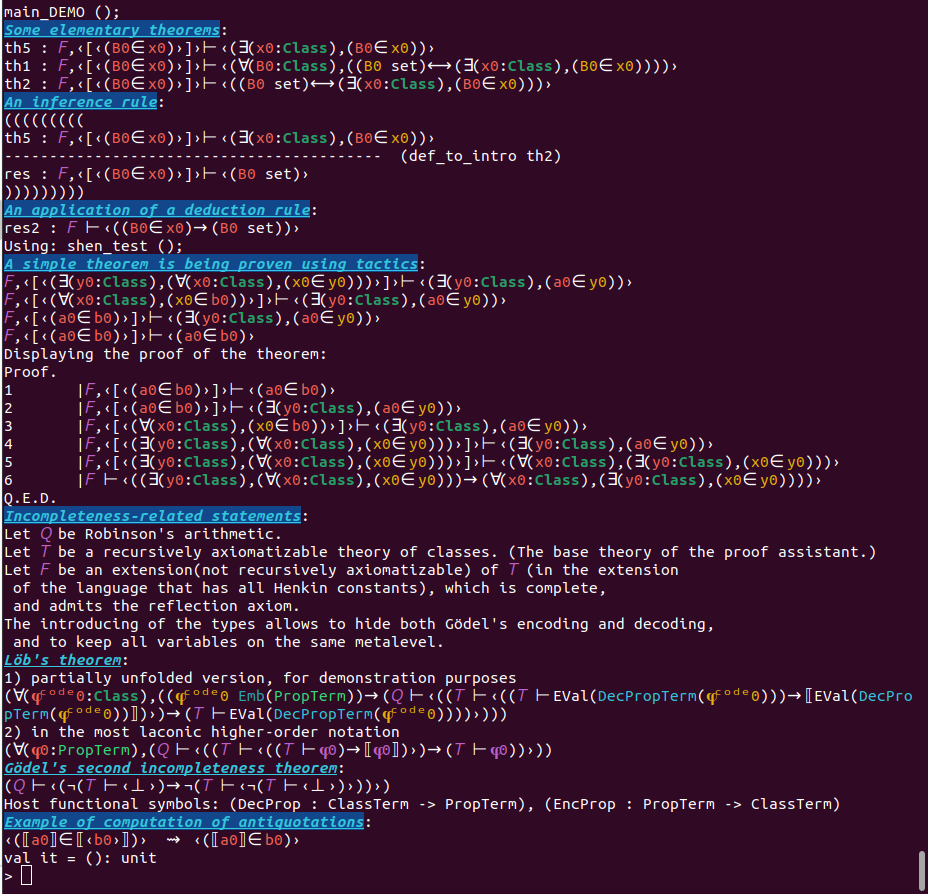
\includegraphics[scale=0.5]{pictures/DEMO.png}

%\restoregeometry
\pagebreak
%\newgeometry{left=1cm, right=3cm, top=3cm, bottom=3cm} 

\section{Type theory of the proof assistant}
The book also documents a proof assistant. Its architecture is inspired by the
LCF approach: a small kernel controls the construction of certified theorems,
while higher-level code organises proofs. The type notation below describes
syntactic objects manipulated by that implementation. It must be distinguished
from the classes and types discussed inside an object theory.

%\iffalse
\IfFileExists{../set_theory_prover/program/CONTENT.ML}{%
\begin{nolinenumbers}
\lstinputlisting[basicstyle=\ttfamily\footnotesize]{../set_theory_prover/program/CONTENT.ML}
\end{nolinenumbers}
}{%
\begin{note}[companion implementation]
The full datatype listing belongs to the companion proof-assistant project
and is not included in this checkout. The definitions and notation below
provide the reading conventions needed for this chapter.
\end{note}
}
%\fi

\restoregeometry
\subsection{Primitive definitions and notation}
\begin{definition}[variable]
A \textit{variable} is an ordered pair consisting of a string, called its \textit{name}, and a natural number, called its \textit{level}. The two components record the identifier and its metalevel in the syntactic representation.
\end{definition}
The companion code gives the corresponding datatype constructors. The mathematical notation below suppresses some of those constructors, so the translation conventions are stated explicitly. %(Especially during the development.)\\
%For any variables $x$,$\phi$,\dots , define
%\subsection{Meaning of dots and bold symbols}%Second bold notation
The following examples connect the typed notation of the implementation with ordinary mathematical notation.
%this subsection. 
%the following subsection.

The comparison begins with representability in arithmetic, then records the proposed encoding in the notation of this book:
\begin{definition*}[representability in the traditional notation]
Let $\mathbb{N}$ be the set of natural numbers. A %first--order
theory $T$ in the language of arithmetic containing $\mathsf{Q}$ ``represents'' the $k$--ary recursive function $f: \mathbb{N}^k\rightarrow\mathbb{N}$ if there is a formula $\varphi_f(x_1, \dots, x_k, y)$ in the language of $T$ s.t. for all $m_1, \dots, m_k \in \mathbb{N}$, if $f(m_1, \dots, m_k) =  n$ then \[
T \vdash \forall y (\varphi_f (\overline{m_1}, \dots, \overline{m_k}, y) \iff y = \overline{n} ).
\]
(\url{https://en.wikipedia.org/wiki/Diagonal_lemma#Representation_Theorem})
\end{definition*}
\begin{example*}[representability in the proposed higher-order notation]
The displays below explore how to encode the preceding definition. Their
intended common meaning is the preceding representability condition. A fully
typed translation still requires the domains of quotation, antiquotation,
and substitution to be fixed; the displays are not separate representation
theorems.
Let $\mathbb{N}$ be the set of natural numbers. 
A% first--order
 theory $T$ in the language of arithmetic containing $\mathsf{Q}$ ``represents'' the $k$--ary recursive function $f: \mathbb{N}^k\rightarrow\mathbb{N}$ if there is a formula $\varphi_f(x_1, \dots, x_k, y)$ in the language of $T$ s.t. 
for all $m_1, \dots, m_k \in \mathbb{N}$, if $f(m_1, \dots, m_k) =  n$ then 
\iffalse
\[
T \vdash \Quote\Fm(\forall y (\Antiquote\Fm(\varphi_f)[\Antiquote\Class(m_1)/x_1, \dots, \Antiquote\Class(m_k)/x_k, y/y] \leftrightarrow (y = \Antiquote(n)) )).
\]
\fi
\[
T \vdash \Quote\Fm(\forall y (\Antiquote\Fm(\varphi_f[m_1/x_1, \dots, m_k/x_k, \Quote(y)/y]) \leftrightarrow (y = \Antiquote(n)) )).
\]
A proposed alternative display, whose typing remains to be checked, is
\[
T \vdash (\forall \Quote(y), ((\varphi_f[m_1/x_1, \dots, m_k/x_k, \Quote\Class(y)/y]) \iff (\Quote\Class(y) = n) )).
\]
Another proposed display is
\[
T \vdash (\forall y, ((\varphi_f[m_1/x_1, \dots, m_k/x_k, \Quote\Class(y)/y]) \iff (\Quote\Class(y) = n) )).
\]
For comparison, the shorter assertion notation is:
\[
T \vdash \llcorner \pmb{\varphi} \lrcorner
\]

The corresponding expanded display is
\[
T \vdash \llcorner
\pmb{ \forall } \pmb{y} \pmb{(}\pmb{\varphi}_{\pmb{f}} \pmb{(}\boldmeta{m_1}\pmb{,} \pmb{\dots}\pmb{,} \boldmeta{m_k}\pmb{,} \pmb{y}\pmb{)} \pmb{\leftrightarrow} \pmb{y} = \boldmeta{n} \pmb{)}\lrcorner,
\]
where
\[
\ulcorner\cdot\urcorner \equivdef (\text{AntiquoteClass} \circ \EncFm),
\]
\[
\ulcorner\cdot\urcorner : \Fm \to \Class
\]
\[
\llcorner\cdot\lrcorner \equivdef (\DecFm \circ \text{QuoteClass}).
\]%(\DecFm \circ \text{QuoteClass})
%\DecFm
\[
\llcorner\cdot\lrcorner : \ClassTerm \to \Fm
\]
For any formula $\phi$,
\[
\llcorner\ulcorner\phi\urcorner\lrcorner
\equiv
\phi.
\]
\end{example*}
\begin{example}[extension rule]
The following proposed \textit{extension rule} records a further design question.
The question marks mark domains that have not yet been specified:
\[
\forall (\varphi:\Fm),\ %
(\Fau \vdash \forall (n:?),\ \llcorner \pmb{\varphi}(\boldmeta{n}) \lrcorner)
\IMPLIES
(\Fau \vdash \forall (n:?),\ \varphi(n) ),
\]
\[
\forall (\varphi:\Fm),\ %
(\forall (n:\ClassTerm),\ \Fau \vdash \llcorner \pmb{\varphi}(\boldmeta{n}) \lrcorner)
\IMPLIES
(\Fau \vdash \forall (n:\Class),\ \varphi(n) ),
\]

Here the operation denoted by $\varphi(n)$, the domains of the two quantifiers,
and the hypotheses licensing passage from all instances to a universal
statement remain to be defined. This example is a proposed rule, not an
admissibility result.
\end{example}

\iffalse % VERY GOOD, BUT DISTRACTING
\subsection{First bold notation}
\subsubsection{Notation for variables}
\begin{notation}[bold variables for terms]
For any lower-case Latin letter(e.g. `x'), define a bold lower-case Latin letter to denote

%val xb1 : Class = (CShiftClass (Quote(CV (namelvl (`x',zero)))))
\begin{lstlisting}
val xb1 : Class = (QuoteClass (CV (namelvl (`x',zero))))
val yb1 : Class = (QuoteClass (CV (namelvl (`y',zero))))
...
\end{lstlisting}
Equivalently, suppressing datatype constructors in the mathematical notation,
\[
\pmb{x} \equivdef \Quote\Var( x_{(0)} ),
\]
\[
\pmb{y} \equivdef \Quote\Var( y_{(0)} ),
\]
\[
\dots
\]
\end{notation}%and so on.

\begin{notation}[bold variables for formulas]
For any lower--case Greek letter(`{$\phi$}',`{$\psi$}', `{$\chi$}', \dots), define a bold lower-case Greek letter to denote
\begin{lstlisting}
val phib1 : Class = (QuoteFm (FmVar vphi))
val psib1 : Class = (QuoteFm (FmVar vpsi))
...
\end{lstlisting}
Equivalently, suppressing datatype constructors in the mathematical notation,
\[
\pmb{\phi} \equivdef \Quote\Fm( \phi_{(0)} ),
\]
\[
\pmb{\psi} \equivdef \Quote\Fm( \psi_{(0)} ),
\]
\[
\dots
\]
\end{notation}

\subsubsection{Notation for functional and predicate symbols}
All bald functional and predicate symbols written boldly simply mean the same constructors as their thin counterparts.
\pagebreak

\fi %VERY GOOD BUT DISTRACTING (First bold notation)

\subsection{Meaning of dots and bold symbols}%Second bold notation
%The second bold notation may be introduced in a situation when it is useful to show that 
The intended translation represents higher-order syntax by first-order codes,
using encoding/decoding together with quotation/antiquotation. The identities
below specify the intended behaviour on well-formed inputs; they do not by
themselves establish a translation theorem for the entire framework.

This subsection uses $\Fm$ as the running example. Analogous conventions are intended for the other syntactic types: $\Ctx$, $\Class$, $\Theory$, etc.%labeled by : for
\begin{definition}[functions Bold and Dot]
Let $\circ$ be an infix operator of composition of functional symbols here. Then
\[
\text{BoldFm} \equivdef \EncFm
\]%(\EncFm \circ \text{QuoteFm})
\[
\text{BoldFm} : \Fm \to \ClassTerm 
\]
and
\[
\text{Dot} \equivdef (\text{AntiquoteClass}).%\circ \DecFm
\]
\[
\text{Dot} : \ClassTerm \to \ClassTerm 
\]

\end{definition}

\begin{notation}[bold and/or dotted variables for formulas]
For a formula variable $\phi$, its encoding is denoted as a bold $\pmb{\phi}$:
\[
\pmb{\phi} \equivnot \text{BoldFm}(\phi).
\]
For any class variable $t$, its antiquotation is denoted with a dot:
\[
\meta{t} \equivnot \text{Dot}(t).
\]
\end{notation}

\begin{note}[non--commutativity of notation]
%Contrary to the first notation,
Boldface and a dot denote operations applied in a specified order:
%\iffalse good
\iffalse
\[
\meta{\pmb{\phi}} \equivdef \text{BoldFm}(\text{DotFm}(\phi)).
\]
\fi
\[
\meta{\pmb{\phi}} \equivnot \text{Dot}(\text{BoldFm}(\phi)).
\]
%where
\iffalse
\[
\text{BoldFm} \equivdef (\EncFm \circ \text{Quote})
\]
and
\[
\text{DotFm} \equivdef (\text{Antiquote} \circ \DecFm).
\]
\fi
After the corresponding decoding step, the round trip is intended to recover the original formula:
\iffalse
\[
\meta{\pmb{\phi}} 
\equiv 
((\EncFm \circ \Quote) \circ (\Antiquote \circ \DecFm))(\phi)
\equiv
\phi
\]%\EncFm(\Antiquote(\phi))

\[
\meta{\pmb{\phi}} 
\equiv 
((\DecFm \circ \Quote) \circ (\Antiquote \circ \EncFm))(\phi)
\equiv
\phi
\]%\EncFm(\Antiquote(\phi))
\fi
\iffalse %last before three--agreement
\[
\meta{\pmb{\phi}} 
\equiv 
(
(\DecFm \circ \text{QuoteClass})
\circ
(\text{AntiquoteClass} \circ \EncFm)
)(\phi)
\equiv
\phi
\]%\EncFm(\Antiquote(\phi))
No!%(\DecFm \circ \text{QuoteClass})
\fi
\[
\llcorner
\meta{\pmb{\phi}} 
\lrcorner
\equiv 
(
(\DecFm \circ \Quote\Class)
\circ
(\text{AntiquoteClass})%\circ \DecFm
\circ
(\EncFm)
)(\phi)
\equiv
\phi
\]%\EncFm(\Antiquote(\phi))
%%%(\text{AntiquoteClass} \circ \DecFm)

So the following computational equality is an identity:
\[
\boxed{
\llcorner
\meta{\pmb{\phi}} 
\lrcorner
\equiv 
\phi
}
\]
%\[
%\pmb{\dot{\phi}} \equivdef \text{Bold}(\text{Meta}(\phi))
%\] % too ugly
\end{note}

\subsubsection{Notation for variables}
\begin{notation}[bold variables for terms]
For a lower-case Latin letter, such as ``x'', boldface denotes the encoded variable:
\iftrue
\begin{lstlisting}
val xb : Class = (EncClass (CV (namelvl ("x", Nat.zero))))
val yb : Class = (EncClass (CV (namelvl ("y", Nat.zero))))
...
\end{lstlisting}
\fi
\begin{lstlisting}
\end{lstlisting}
Equivalently, suppressing datatype constructors in the mathematical notation,
\[
\pmb{x} \equivdef \EncClass(x_{(0)} ),
\]
\[
\pmb{y} \equivdef \EncClass( y_{(0)} ),
\]
\[
\dots
\]
\end{notation}%and so on.

\begin{notation}[bold variables for formulas]
For any lower--case Greek letter(`{$\phi$}',`{$\psi$}', `{$\chi$}', \dots), define a bold lower-case Greek letter to denote
\begin{lstlisting}
val phib : Class = (EncFm (FmVar vphi))
val psib : Class = (EncFm (FmVar vpsi))
...
\end{lstlisting}
Equivalently, suppressing datatype constructors in the mathematical notation,
\[
\pmb{\phi} \equivdef \EncFm(\phi_{(0)} ),
\]
\[
\pmb{\psi} \equivdef \EncFm(\psi_{(0)} ),
\]
\[
\dots
\]
\end{notation}

\subsubsection{Notation for functional and predicate symbols}
Bold function and predicate notation denotes constructors acting on codes.
Encoding is therefore described inductively, one syntactic constructor at a time:

\begin{definition}[computation of the encoding of statements]
For a theory term $\Wau$, a context term $\Gamma$, and a formula term $\phi$,
\[
\EncStmt(\Wau,\,\Gamma\vdash \phi)
\equiv
\pmb{(} \EncTheory(\Wau) \pmb{,}\, \EncCtx(\Gamma)\pmb{\pmb{\vdash}} \EncFm(\phi)\pmb{)}
\]
\end{definition}
The right-hand side applies a first-order function symbol to the codes of the
three arguments. Its value represents the code of the whole statement. Other
syntactic constructors are encoded in the same way.

\iffalse
\begin{definition}
A term is called a \textit{class--term}, when it's a term of the type which is, unfortunately confusingly, called $\Term$ in the source code.
\end{definition}
\fi


\subsection{Definitions of inference--related constants and their notation}
\iffalse
\subsection{OBSOLETE PART TO BE DELETED}

\begin{definition}[informal introduction]
Let $\Fm,\ClassTerm,\Ctx,\Theory,...$ be a finite amount of sets, consisting of formulas, terms, contexts, theories, etc, in a model of Standard ML language. There is a model, and the precise construction of it is outside of the scope of this book,let's just assume that there is one, and therefore there is one in a foundational theory $\Fau$, so there is a (computable) function from syntactic entities  to certain objects in a domain of discussion $C$, which is a conglomerate of all classes.\\

In a such model of Standard ML, there is a typing relation between semantics of terms and types.\\
Assume this relation is given.\\
Then let's restrict it, for simplicity, to only those aforementioned types $\Fm,\ClassTerm,\Ctx,\Theory,...$ and their ground values (without variables).\\
Then let's extend this typing relation to the extended one, in which all remaining types also have type $\Type$, such that 
$(\Fm:\Type)$, $(\Class:\Type)$, $(\Ctx:\Type)$, $\dots$
%, $(\Typ:\Typ)$ (note the last one).\\
This could lead to a contradiction (Girard's Paradox) in case if this typing system would be significantly richer: at least if it had types of functions, dependent types, etc, but it doesn't have any of that: it is as simple as possible.
\end{definition}
%, even finite.
\fi

%class constants, corresponding to codes of syntactic entities
\begin{definition}[sets of codes]
%Let $\circ$ be a composition of functional symbols here, then t
The following class constants represent the codes of formulas, class terms, contexts, and the other syntactic datatypes:
\[
\text{FmCode} 
\equivdef
\CFm
\text{, where }
\CFm
\equivdef
\Emb(\TFm)
\]
\[
\text{ClassCode} 
\equivdef
\CClass
\text{, where }
\CClass
\equivdef
\Emb(\TClass)
\]
\[
\dots
\]
\end{definition}
\iffalse
\begin{notation}[overloading]
Luckily, on paper, it is possible to completely avoid the necessity of coloring the constants or of writing prefixes, via simple overloading trick: 
\[
\text{FmCode}
\equivnot
\CFm
\]
\[
\text{ClassCode}
\equivnot
\CClass
\]
\[
\dots
\]
Unfortunately, the Standard~ML doesn't have the overloading feature, so prefixes are kept in the program.
\end{notation}
\fi


%(\text{Enc}\circ\text{VTyp})

%It is possible for
%\TClass is an element


\iffalse
\begin{notation}[abuse of notation]
It seems possible to identify $\ClassTerm$ and $\TClass$, but it will not be done to avoid confusion.
%The author is not sure, where 
%(but in fact, no)
%It can be
%Starting from the next chapter, it can be 
%It seems like
%\[
%\ClassTerm = \TClass = \text{CClass}
%\]
\end{notation}
\fi
\subsection{Typed quantification and its notation}
Typed quantification over syntactic objects is represented below by
quantification over their codes. A code variable must be fresh for the body,
and every displayed substitution is capture-avoiding. Quantification over
semantic classes is a separate issue: the set- and class-quantifier schemes
later in this subsection are proposed axioms, not consequences of the
coding convention alone.
\begin{definition}[quantifiers with a bound variable of type $\Fm$]
Let $\phi$ be a variable for formulas.\\
Let $\psi$ be a formula.\\
% such that $\phi_code$ is not free in $\phi$.
%Not enough.
Choose a fresh code variable $\phi_\code$. Assume also that the substitution
$\psi[(\DecFm(\phi_\code))/\phi]$ is computed successfully, i.e. without raising an exception or error.
Then
%Then the following formula 
\[
(\forall (\phi:\TFm),\ \psi)
\iffdef
\]
\[
\iffdef
(\forall (\phi_\code:\TClass),\ %
(\phi_\code\in \Emb(\TFm))
\implies
\psi[
\DecFm(\phi_\code)
/
\phi
]
)
\]
\end{definition}
% bad1: (\text{Enc}\circ\text{VTyp})
% bad2: (\text{ValToFm}\circ\text{Dec})
\begin{notation}[naming prefix of labels]
Standard~ML distinguishes type names from values. Here the datatype named
Type has value constructors with the prefix ``T'', such as ``TFm'',
``TClass'', and ``TCtx''. The prefix helps distinguish a syntactic type label
from the datatype of expressions that carry that label.\\
In mathematical displays we suppress the prefix when the context determines
its meaning. Thus, instead of the explicit label
\[
``(\forall(\phi:\TFm),\ \dots)",
\]
starting from the next chapter, it will be written
\[
``(\forall(\phi:\Fm),\ \dots)".
\]
\end{notation}
\iffalse
\begin{notation}[overloading naming prefix of constants]
Similarly, instead of more precise expression
\[
``(\forall(f\in\CFm),\ \dots)",
\]
it will be written
\[
``(\forall(f\in\FmCode),\ \dots)".
\]
Note, that the letter $f$ here is a vareiable for the code of the formula, not for the formula itself, as was above where the symbol ``:'' was used.
\end{notation}
\fi
Other changes between syntactic and semantic notation will be stated explicitly.% at all costs.


%Now the tricky part, te

\begin{axiom}[set terms quantification unfolds via itself]
The proposed set-quantifier scheme retains a set-typed code quantifier:
\[
(\forall (t:\TSet),\ \psi)
\iffaxm
\]
\[
\iffaxm
(\forall (t_\code:\TSet),\ %
(t_\code\in \Emb(\TSet))
\implies
\psi[
\DecSet(t_\code)
/
t
]
)
\]
Here $t_\code$ is fresh for $\psi$. The scheme is stated as an axiom because
the same quantifier appears on both sides; it is not a recursive definition.
Its semantic justification is an additional obligation of this proposed model.
\end{axiom}
\begin{notation}[overloading class bindings]
Again, as previously for formulas, a formula
\[
``(\forall(K:\TSet),\ \dots)"
\]
can be written as
\[
``(\forall(K:\Set),\ \dots)".
\]
\iffalse
and also the quantifiers bound by a variable codes of definable classes
\[
``(\forall(e\in\CClass),\ \dots)"
\]
can be likewise unambiguously written as
\[
``(\forall(e\in\ClassCode),\ \dots)".
\]
\fi
\end{notation}
%########################## Class

\begin{axiom}[class terms quantification unfolds via itself]
The analogous proposed class-quantifier scheme retains a class-typed code
quantifier. Its typing predicate requires the interpretation supplied by the
model of pi-types.
\[
(\forall (t:\TClass),\ \psi)
\iffaxm
\]
\[
\iffaxm
(\forall (t_\code:\TClass),\ %
(t_\code : \Emb(\TClass))
\implies
\psi[
\DecClass(t_\code)
/
t
]
)
\]
Here $t_\code$ is fresh for $\psi$. The scheme is stated as an axiom because
the same quantifier appears on both sides; it is not a recursive definition.
Its semantic justification is an additional obligation of this proposed model.
\end{axiom}
\begin{notation}[overloading class bindings]
Again, as previously for formulas, a formula
\[
``(\forall(K:\TClass),\ \dots)"
\]
can be written as
\[
``(\forall(K:\Class),\ \dots)".
\]
\end{notation}

% ###

\begin{notation}[the default type]
In class-theoretic formulas, an omitted type annotation means ``Class'':
\[
(\forall K,\ \psi)
\iffnot
(\forall (K:\Class),\ \psi)
\]
Thus an unqualified ``term'' in that context means a class term. In discussions
of implementation or syntax, the relevant datatype is stated separately.
\end{notation}
\iffalse% METALANG
\section{Metalanguage[section is not yet finished]}
Usually, when something is proven, questions arise: ``Where it was proven?'', ``What was a foundational theory?'', ``What was a metatheory of the statement?''. Unfortunately, once the answers are established for the theory, the same questions may be asked about metatheory, metametatheory, and so on.\\
To avoid this ``infinite descend'' with increasing complexity of the statement of each step, author proposes to use a certain theory $\mathcal{F}$ as it's own metatheory, so the questions about the metatheory can be discussed in the theory itself.\\%is possible to answer within a theory.\\
In fact, a prefix ``$\mathcal{F}\vdash$'' is virtually omnipresent near every formula of this book, but it is not written, since the act of actual writing of it leads to the increase of complexity and increase of a metalevel of the statement.\\
\begin{definition}[level of meta]
Metalevel of the statement is the maximal amount of nested ``$\mathcal{F}\vdash (\dots)$'' in the formula.
\end{definition}


%Metatheory:\\
During reading the string of symbols, it is important to distinguish entities which are semantic(e.g. a set $\emptyclass$ or a proposition $(\emptyclass \in \omega)$) from their symbols which are syntactic and belonging to metatheory (e.g. a term $\ulcorner\boldemptyclass\urcorner$, and a judgement $(\ulcorner\boldemptyclass\urcorner : \Class)$). The symbols $``\ulcorner\cdot\urcorner"$ are used to explicitly show that that the object inside is syntactic, i.e. is a word. 


%%%%% May be useful:
%%%%% Currently, they are often omitted, but the the rule of thumb is that in chapters devoted to logic, syntactic entities are written, and in chapters devoted to mathematics, semantic entities are written. Moreover, to avoid confusion, and due to computational properties of syntactic entities, it is natural to use a naive type theory for logic parts, so it makes it is easy to distinguish syntax from semantics.


A sufficiently expressive programming language of reader's choice, may be used for implementing functions and structures which operate with terms, formulas, etc.

In this chapter, an elementary type theory is informally used.
Depending on the purposes of the reader, it can be implemented:
\begin{enumerate}
\item either in some programming language, leading to creation of a proof assistant (\url{https://github.com/georgydunaev/class_theory_proof_assistant}),
\item or within the foundations themselves, for example via notions defined in the section ``Classes--as--Types''.
\end{enumerate}



\iffalse
Also the concept of ``quotation'' and ``antiquotation'' is introduced.
\begin{lstlisting}
datatype 'a frag = QUOTE of string | ANTIQUOTE of 'a
\end{lstlisting}
\fi

%In chapters

%, which can be implemented either in programming language(and as a result it wil),
\pagebreak

\fi% METALANG
\iffalse %TODO TAKE THE BEST
\section{Adaptation of a quote from ``Languages and Calculi''}
(This section, is an adaptation and translation of the text from the book ``Languages and Calculi'': \cite[73-74]{vereshchagin_shen_2012})).\\

We fix a certain set of symbols called individual variables. These are intended to denote elements of the set over which the functions and predicates are defined; usually, Latin letters such as $x$, $y$, $z$, $u$, $v$, $w$ with indices are used for this purpose. Each formula will use only a finite number of variables, so a countable set of variables will suffice. We assume that the variables are distinct from all function and predicate symbols of the signature (otherwise confusion would arise).

We define the notion of a term for a given signature. A \textit{term} is a sequence of variables, commas, parentheses, and signature symbols, which can be constructed according to the following rules:
\begin{itemize}
  \item An individual variable is a term.
  \item A function symbol of arity 0 is a term.
  \item If $t_1, \dots, t_k$ are terms and $f$ is a function symbol of arity $k > 0$, then $f(t_1, \dots, t_k)$ is a term.
\end{itemize}
In principle, we could avoid distinguishing function symbols of arity 0 (also called textit{constants}) as a separate group, but then we would have to write parentheses after them (as is done in the C programming language).

If $A$ is a predicate symbol of arity $k$ and $t_1, \dots, t_k$ are terms, then the expression $A(t_1, \dots, t_k)$ is considered an \textit{atomic formula}. Additionally, any predicate symbol of arity 0 is also considered an atomic formula.

Formulas are constructed by the following rules:
\begin{itemize}
  \item An atomic formula is a formula.
  \item If $\varphi$ is a formula, then $(\lnot\varphi)$ is a formula.
  \item If $\varphi$ and $\psi$ are formulas, then the expressions $(\varphi \land \psi)$, $(\varphi \lor \psi)$, and $(\varphi \implies \psi)$ are also formulas.
  \item If $\varphi$ is a formula and $\xi$ is an individual variable, then the expressions $\forall \xi\, \varphi$ and $\exists \xi\, \varphi$ are formulas.
\end{itemize}

In many cases, the signature includes a binary predicate symbol $=$, called \textit{equality}. By tradition, instead of writing $=(t_1, t_2)$, one writes $(t_1 = t_2)$.
\pagebreak
\iffalse %May26
\section{Predicate calculus as an object language [unfinished section]}

In this book, a class theory is being developed and studied, so classes are chosen by author to be the objects of theories $\Tau$ and $\Fau$.

%In this chapter metalevel variables are normal, and metalevel constants are bold.

\begin{metanotation}[styles]
The following style conventions are adopted:
\begin{enumerate}
\item Every bold letter denotes the actual letter of from the alphabet.\\
Examples: `$\pmb{a}$', `$\pmb{b}$', `$\pmb{c}$', etc.
%Examples: $\pmb{a}\ceq$`a', $\pmb{b}\ceq$`b', $\pmb{c}\ceq$`c', etc.
\item Every non--bold, 1--letter word of Greek or Latin alphabet written in ``\textbackslash mathnormal'' style with or without subscript, is a metavariable.
\item Words of greek or latin alphabet written in ``\textbackslash mathrm'' style are constants.
\end{enumerate}
\end{metanotation}
\begin{metanotation}[objects vs metaobjects]%\ \\
In chapters devoted to logic, set/class--theoretics \LaTeX\ symbols are syntactic codes.\\
In chapters devoted to mathematics, set/class--theoretics \LaTeX\ symbols are semantic objects.
\end{metanotation}
\begin{metanotation}[proofs]%\ \\
Proofs are written as lists of imperative commands, which are usually one--liners. They are written in a way, that both the reader (and a parser of a proof assistant that is being developed) can recover the precise meaning of the line without the context of the theorem, and then validate it.
%When something like
E.g.: the following expression has double meaning depending on the choice of metatheory.
\[
(\phi_1 \LAND \phi_2 \IMPLIES \phi_3 )
\]
For theory $\Tau$, it roughly means a constructive existence of computable transformation of a pair of proofs into the third:
\[
``\exists^{\text{constructively}}(p\text{ computable function}),\text{ such that }p:(\Tau,\Gamma\vdash\phi_1)\times(\Tau,\Gamma\vdash\phi_2)\to(\Tau,\Gamma\vdash\phi_3)",
\]
meanwhile for the theory $\Fau$, it simply means a proposition
\[
(\Fau,\Gamma\vdash\phi_1)
\land
(\Fau,\Gamma\vdash\phi_2)
\implies
(\Fau,\Gamma\vdash\phi_3).
\]
In order to avoid the complications of the computation-- and constructivism--related topics, the author tries to stick to the second meaning till the end of the book. Long story short, both the theory and the metatheory are $\Fau$.
\end{metanotation}
%``\\mathnormal'' style
%All inductive definitions in this section are also simultaneous, since formulas depend on terms and vice versa.

%\begin{definition}[$\BddExpr$]%\ \\
%Inductive definition of bound expressions:
%\begin{enumerate}
%\item $(x:\Var)\ ,\ (A:\alpha) \Implies ((x.A):\Class)$.
%\end{enumerate}
%\end{definition}

\begin{lstlisting}
type DottedString = (Alphabet * Nat) List
\end{lstlisting}

%The well--establishe name ``antiquotation'' is quite unfortunate.
\begin{lstlisting}
datatype 'a Fragment = QUOTE of string | ANTIQUOTE of 'a
\end{lstlisting}

\begin{lstlisting}
type Code = (Syntax Fragment List)
\end{lstlisting}

\begin{metadefinition}[syntax]
\[
\text{Syntax} \eqdef \ClassTerm \sqcup \Fm \sqcup \BClass \sqcup \dots
\]
\end{metadefinition}

%\[
%\text{Syntax} \eqdef \Fm \sqcup \dots 
%\]
\begin{metadefinition}[encoding(todo:rewrite these definitions)]
This definition is a simplified variant of G\"odel's numbering, since for the purposes of this book it is unnecessary to encode syntactic entities(terms, formulas, etc) with natural numbers.
\[
\# : (\text{Syntax Frag List}) \to \text{Syntax}
\]
The function $\#$ may raise an exception if the raw string take as argument is ill--formed, i.e. if it doesn't follow certain fixed syntactic rules.\\
It 
\end{metadefinition}
%\[
%\# \:  \text{(Syntax Frag List)} \to \Class)
%\]
\[
`` \cdot " \: \to \text{DottedString} 
\]
%\to \text{(Syntax Fragment List)}

\[
\myparse \: \text{DottedString} \to \text{(Syntax Fragment List)}
\]

%\[
%???`` \cdot " \: \text{DottedString} \to \text{(Syntax Fragment List)}
%\]

\begin{metadefinition}[parsing function for a string with metavariables(todo:rewrite these definitions)]
\[
\myparse : \DottedString \to (\text{Syntax Frag List})
\]
\end{metadefinition}
The parsing function satisfies the following computation rule:\\
\begin{metainferencerule}[(todo:rewrite these definitions)]
%For all $A\in(\text{Syntax Fragment List})$, 
For all $A\in(\text{Syntax})$,
\[
A \equiv \myparse(\myquote{\meta{\pmb{A}}}).
\]

\[
A \equiv \myparse(\myquote{A}).
\]
\end{metainferencerule}

\iffalse
A string representation of the formula is divided into fragments, so it is a list of fragments of what? Of syntactic entities. It is indeed, because a metavariable may be used to represent literally anything syntactic in the formula: a term, a variable(as before), a subformula, etc.
\fi



\iffalse GOOD BUT TOO COMPLICATED FOR THIS PART
If dependent types are allowed, then
\[
\FuncSymb : \sum_{n:\N}((\{1,\dots,n\}\to \Class)\to \Class),
\]
\[
\PredSymb : \sum_{n:\N}((\{1,\dots,n\}\to \Class)\to \Fm).
\]
If not, then certain formulas become ill-formed, and need to be checked.
\fi
\begin{metanotation}[meaning of typing relation]
Bold mathematical symbols are just text, like ``string'' in programming languages. Thin symbols are various meta--level functions.
A string of the form $(s:A)$ is a notation for 
%$(x \in A)$.\\%\ulcorner x \urcorner
%$(\ulcorner x \urcorner \in A)$.\\%\ulcorner x \urcorner
%$((\#s) \in A)$.\\%\ulcorner x \urcorner
%Maybe even 
$((\#s) \in (\#A))$.%(ToDo).%\ulcorner x \urcorner
\end{metanotation}
\begin{metanotation}[meaning of symbol's boldness]
Thin symbols are used for depicting functional symbols on object level.\\
Bold symbols are used for depicting a meta--level application of the functions, which construct a syntactic object be applying the functional symbols to the arguments.
\end{metanotation}
\pagebreak
\fi %May26
\begin{metanotation}[metasyntax for constructors inside the quoted text]
When dealing with variables, it is possible to use these definitions:
(The following definitions are needed to avoid syntactic monsters with lots of dots like this one: ``$\boldccc{\meta{x}}{\meta{t}}{\meta{\phi}}$''.)
\iffalse
\[
\pmb{\bm{\bot}}
\eqdef
%\left\ulcorner
\bot
%\right\urcorner
\]
\[
%\bm{\{ }
\boldccc{x}{t}{\phi}
%\raisebox{-2.5pt}{\rule{1.5pt}{10pt}}
\eqdef
%\left\ulcorner
\ccc{\meta{x}}{\meta{t}}{\meta{\phi}}
%\right\urcorner
\]
\fi
\[
\bot
\equivnot
%\left\ulcorner
``
\boldbot
"
%\right\urcorner
\]
\[
\emptyclass
\equivnot
\myquote{
\pmb{\emptyclass}
}
\]
\[
\thinneg{A} \equivnot ``\boldneg{\meta{A}}"
\]
\[
\ccc{x}{t}{\phi}
\equivnot
%\left\ulcorner
``
\boldccc{\meta{x}}{\meta{t}}{\meta{\phi}}
"
%\right\urcorner
\]

\begin{notation}[dot]
If a variable of an arbitrary type has dots on top of it, it means, that it is from higher meta--level.\\
The number of dots on top of the variable means how many times "meta" this variable is.\\
Dots are used for variables only.\\
\[
\meta{\phi} \equivnot \Antiquote(\phi)
\]
\end{notation}


\iffalse
\begin{notation}[bold var]
If a letter is written bold, it means only this particular variable, which is not possible to substitute with other variables or terms.
\end{notation}
\fi
\begin{notation}[bold text variable means no terms]
If a variable is written as a bold letter, it means it is possible to substitute it only with other variable from the same collection of variables used for particular type.
\end{notation}


\begin{notation}[displaying in computer's terminal]
It is a bit tricky to display dots in Linux terminal, so the following notation may be used.
\[
\pmb{\phi}^\text{code} \equivnot \EncFm(\pmb{\phi})
\]% \meta{\pmb{\phi}}(BAD)
\end{notation}

\begin{definition}[translation of variables for formulas]% into the language]
%(This is a main definition.)

For each variable with a name in the group ``a lowercase letter of Greek alphabet'',

\iffalse
(in case of type of formulas, a name is

Let $\phi$

\fi

\[
\pmb{\phi}
\equivdef
\DecFm(\pmb{\phi}^\code)
\]
\[
\text{Meta}(\pmb{\phi})
\equivdef
\meta{\pmb{\phi}}
\]
\[
\EncFm(\meta{\pmb{\phi}})
\reductsto
\pmb{\phi}
\]


(There is no need to additionally require that
\[
\pmb{\psi}
\equivdef
\DecFm({\pmb{\psi}^\code})
,\ %
\pmb{\chi}
\equivdef
\DecFm({\pmb{\chi}^\code})
,\ %\dots;
\]
because the agreement of bold notation requires it automatically. The group ``Greek lowercase letters'' is associated with type of formulas.)


%\equivdef
%\DecFm(\pmb{\phi}^{\text{code}})
\iffalse
Each variable of type Fm is defined like this.
Each time, there is a small Greek letter, it means the following. 
\fi
\end{definition}
\iffalse
For every formula--variable $\meta{\phi}$ of metalevel strictly higher than zero,
\fi
\begin{note}[formula vs formula term]
The main distinction between \underline{formulas} and \underline{formulas terms} is that while they are both syntactical objects of type $\Fm$, but a \underline{formula} doesn't contain any of $\Enc$ and $\Dec$ constructors(for any of the types), while the \underline{formula term} may have them.
\end{note}
\begin{axiom}
For every variable $\pmb{\phi}$ of type ``formula'', there exists a variable  $\pmb{\phi}^\code$ of type ``class--term''.
\end{axiom}
\begin{definition}[encoding variables for formulas]
The axiom above allows the function for encoding the formulas defined to be computed in the following way:
\[
\EncFm(\pmb{\phi})
\equivdef
{\pmb{\phi}}^\code
\]
\end{definition}
\begin{definition}[further encoding for formulas]
For any \underline{formulas}'s terms $\phi$ and $\psi$, the function for encoding the formula is computed this way:
\[
\EncFm((\phi \implies \psi))
\equivdef
\pmb{(}\EncFm(\phi) \pmb{\implies} \EncFm(\psi)\pmb{)}
\]
A bold writing schrift of a predicate symbol notation symbols here means that, if the number of dots is interpreted simply like just a part of the variable's name, then it will be a first--order predicate symbol occurrence in a first--order class term. (After the encoding of both subformulas will be fully computed, of course.)
\end{definition}

\begin{theorem}[]
For any formula terms $\phi$,
\[
(\DecFm(\EncFm(\phi)) \reductsto \phi)
\]
(without proof via structural induction)
\end{theorem}

%If a variable of an arbitrary type is being encoded, then the the quotation marks are used for brevity.\\
For example, if a class--term $t$ is an occurrence of a variable $\pmb{x}$, then

Left and right sides of these definitional equalities are computationally equivalent.(Conversions)
TODO: DOUBLE CHECK HERE
\[
t\equiv \DecClass(\EncClass(t))
\]
%\forall t^{code}
\[
\forall (t:\Class),
(t\equiv \DecClass(\EncClass(t)))
\]
\[
\forall (\phi:\Fm),
(\phi\equiv \DecFm(\EncFm(\phi)))
\]
\[
\forall (\phi^{\text{code}}:\Class),
(\phi^{\text{code}} \in \text{Emb(Fm)})
\implies
(\phi\equiv \DecFm(\phi^{\text{code}}))
\]




\[
(\pmb{\phi}:\Fm)
\]

There is an agreement, that for each variable,
\[
\phi^{\text{code}}
\equiv
\EncClass(\phi)
\]


\[
t\equiv \DecClass(\meta{t})
\]



\[
``\meta{t}"
\equiv
``\pmb{x}"
\equivnot
\EncClass(\pmb{x})
\equiv
\EncClass(t)
\]

\[
``x"\equivnot \EncClass(x) 
\]
\[
\meta{x}\equivnot \DecClass(x) 
\]


(and so on\dots)
\end{metanotation}


\begin{metadefinition}[set of terms of type $\ClassTerm$]%\ \\
The inductive definition of terms:
\begin{enumerate}
%\item $(x:\Var(\Class)) \Implies (x:\Class)$.
%\item $(bt:\BClass) \Implies ((x\mapsto t):\BClass)$.
%\item $(x:\Var)\ ,\ (\phi:\Fm) \Implies (\cc{x}{\phi} :\Class)$.
%\item $(\mathbf{x}:\Var)\ ,\ (\mathbf{t}:\Class)\ ,\ (\boldsymbol{\phi}:\Fm) \Implies (\ccc{x}{t}{\phi} :\Class)$.
\item $(x:\Var)\ ,\ (t:\Class)\ ,\ (\phi:\Fm) \Implies (\ccc{x}{t}{\phi} :\Class)$.
\[
\text{ClassCompr}_1 : (\ClassTerm, (\ClassTerm \times \Fm))\ \Bound \to \Class
\]
\item $(\vv{x}:\text{Var List})\ ,\ (t:\Class)\ ,\ (\phi:\Fm) \Implies (\ccc{\vv{x}}{t}{\phi} :\Class)$.
\[
\text{ClassCompr} : (\ClassTerm, (\ClassTerm \times \Fm))\ \text{BoundByList} \to \Class
\]

\iffalse
\item $(f:\FuncSymb)\ ,\ (t_1:\Class)\ ,\ \dots\ ,\ (t_n:\Class) \Implies (f(t_1,\dots,t_n):\Class)$.
\item $(x:\Var)\ ,\ (A:\Fm) \Implies ((\varepsilon x.A):\Class)$.
\item $(x:\Var)\ ,\ (A:\Fm) \Implies ((\iota x.A):\Class)$.
\fi
\end{enumerate}
\end{metadefinition}
\begin{metadefinition}[set of formulas $\Fm$]%\ \\
The inductive definition of formulas:
\begin{enumerate}
%\item $(A:\Var(\Fm)) \Implies (A:\Fm)$.
\item $(\bot:\Fm)\ ,\ (\top:\Fm)$. %\ ,\ (\ddagger:\Fm)$.
%\item $(P:\PredSymb)\ ,\ (t_1:\Class)\ ,\ \dots\ ,\ (t_n:\Class) \Implies (P(t_1,\dots,t_n):\Fm)$.
\item $(t_1:\Class)\ ,\ (t_2:\Class) \Implies (\thinin{t_1}{t_2}:\Fm)$.
\item $(t_1:\Class)\ ,\ (t_2:\Class) \Implies ((t_1=t_2):\Fm)$.
%(\pmb{(}t_1\pmb{\in} t_2\pmb{)}:\Fm).
% TODO
%\[
%\thinneg{A} \equivnot ``\boldneg{\meta{A}}"
%\]
\item $(\phi:\Fm) \Implies (\thinneg{\phi}:\Fm)$.
\item $(\phi:\Fm)\ ,\ (\psi:\Fm) \Implies (\thinimplies{\phi}{\psi}:\Fm)$.
% (\pmb{(}A\pmb{\implies} B\pmb{)}:\Fm)
\item $(\phi:\Fm)\ ,\ (\psi:\Fm) \Implies (\thinand{\phi}{\psi}:\Fm)$.
\item $(\phi:\Fm)\ ,\ (\psi:\Fm) \Implies (\thinor{\phi}{\psi}:\Fm)$.
\item $(x:\Var)\ ,\ (\phi:\Fm) \Implies (\thinforall{x}{\phi}:\Fm)$.
\item $(x:\Var)\ ,\ (\phi:\Fm) \Implies (\thinexists{x}{\phi}:\Fm)$.
%\item $(x:\Var)\ ,\ (\phi:\Fm) \Implies ((!x.\phi):\Fm)$.
\iffalse
\item $(t:\Class) \Implies (\pmb{(}t \bm{\lexists}\pmb{)}:\Fm)$.
\item $(t:\Class) \Implies (\pmb{(}t \bm{\lunique}\pmb{)}:\Fm)$.
\fi
%\item $(x:\Var)\ ,\ (A:\Fm) \Implies ((h_{(x.A)}):\Class)$.
\item $(x:\Var)\ ,\ (\phi:\Fm) \Implies (\thinepsilon{x}{\phi}:\Class)$.%(\pmb{(}\bm{\Henkin} x\bm{,}A\pmb{)}:\Class).
\end{enumerate}
\end{metadefinition}
\begin{metadefinition}[$\BClass$]%\ \\
The inductive definition of bound terms:%\pmb{(}x\bm{,}t\pmb{)}
\item $(x:\Var)\ ,\ (t:\Class) \Implies (\thincomma{x}{t}:\BClass)$.
\end{metadefinition}
\begin{metadefinition}[$\BFm$]%\ \\
The inductive definition of bound formulas:%pmb{(}x\pmb{,}\varphi\pmb{)}
\item $(x:\Var)\ ,\ (\varphi:\Fm) \Implies (\thincomma{x}{\varphi}:\BFm)$.%\mapsto
\end{metadefinition}


\iffalse
\begin{definition}[quotation of a]
Quotation:
\[
\ulcorner\cdot\urcorner : \String \to \Class
\]
\end{definition}
\begin{definition}
Antiquotation:
\[
\llcorner\cdot\lrcorner : \ClassTerm \to \String 
\]
\end{definition}
\fi
\begin{metadefinition}[free variables of]
The function, which returns the free variables of a syntactic object, e.g. of the term:(ToDo)
\[
\FV : \text{Syntax} \to \List(\Var)
\]
\[
\FV(\ulcorner\emptyclass\urcorner)\eqdef \emptylist
\]%\emptyclass
\iffalse
\[
\forall (x:\Var),\ %
\forall (A:\Fm),\ %
\FV(\ulcorner(\exists \meta{x},\ \meta{A})\urcorner)\eqdef \FV(A)\setminus\{x\}
\]%\emptyclass
\[
\FV(\ulcorner(\exists \meta{x},\ \meta{A})\urcorner)\eqdef \FV(A)\setminus\{x\}
\]
\[
\FV(\pmb{(\exists}x\pmb{,}\ A\pmb{)})\eqdef \FV(A)\setminus\{x\}
\]
\fi
\[
\forall (x:\Var),\ %
\forall (A:\Fm),\ %
\FV(\ulcorner\boldexists{ \meta{ x } }{\meta{ A } }\urcorner)\eqdef \FV(A)\setminus\{x\}
\]%\emptyclass

\[
\FV(\#``\boldexists{ \meta{ x } }{\meta{ A } }")\eqdef \FV(A)\setminus\{x\}
\]

\[
\FV(\#\thinexists{x}{A})\eqdef \FV(A)\setminus\{x\}
\]

\iffalse
\[
\FV_\ClassTerm : \ClassTerm \to \List(\Var)
\]
\[
\FV_\Fm : \Fm \to \List(\Var)
\]
\fi
 %\Pow_{\text{fin}}%\Finite\Set\List
\subsubsection{Theory and context}
\begin{definition}[context]%\ \\meta
Context is a finite list of arbitrary formulas. It is usually denoted by the uppercase Greek alphabet letters like $\Gamma$ or $\Delta$.
\end{definition}
\begin{definition}[theory]%\ \\meta
Theory is an ordered (usually infinite) set of closed formulas. It is denoted by italic uppercase Latin alphabet letters like $\Tau$, $\Wau$ or $\Fau$.
\end{definition}





\begin{metadefinition}[definitional equality]
Let $t_1$ and $t_2$ be terms, such that $t_1$ is (normally) an application of a (new) functional symbol to some arguments.\\
Assume(normally) that $t_2$ has no free variable which are not free in $t_1$.\\
Then the formula $(t_1 \eqdef t_2)$ is a notation for $(\text{closure}(t_1 = t_2))$ and a ceertain assumption on aleading functional symbol of $t_1$.
\end{metadefinition}
\begin{example}[definitional equality in the definition of the powerclass]
For example, the formula
\[
\power X \eqdef \cc{Y}{Y\subclass X}
\]
means
\[
\forall (X:\Class),\ \ulcorner\pmb{\power} X\urcorner \in\Class
\]
and
\[
\forall X,\ \power X = \cc{Y}{Y\subclass X}.
\]
(This is done to avoid writing a closure operator in definitions, which is necessary, sine technically axioms are declared, which are formulas of the theory, so they must be without free variables.)
\end{example}

\begin{metadefinition}[definitional equivalence]
Similarly to the previous definition, let $\phi_1$ and $\phi_2$ be formulas, such that $\phi_1$ is (normally) an application of a (new) predicate symbol to some arguments.\\
Assume(normally) that $\phi_2$ has no free variable which are not free in $\phi_1$.\\
Then the formula $(\phi_1 \iffdef \phi_2)$ is a notation(or a definition?) for $(\text{closure}(\phi_1 \iff \phi_2))$.
\end{metadefinition}
%It may be reasonable to require that 

\begin{definition}[primitive proof(todo)]%\ \\
Primitive proof is a finite list of formulas, such that each is derivable in the theory with a context of all previous formulas.
\end{definition}
\begin{notation}[derivablity from a theory with the empty context]
Let $\Wau$ be a theory, and $\phi$ be a formula, then it is convenient to write
\[
(\Wau \vdash \phi) \iffdef (\Wau, [\,] \vdash \phi)
\]
\end{notation}

\begin{example}
Assume $\Tau$ is a \textbf{finite} theory, and $\Gamma$ is a context, then
\[
\left(\Tau,\Gamma\vdash \phi\middle) \iff \middle(\middle(\bigwedge \Tau\middle)\land \middle(\bigwedge \Gamma\middle)\implies \phi\right)
\]
Note, that theory normally \underline{may not be finite}, so this equivalence holds extremely rarely. %does not always work
\end{example}


(todo: write the standard definitions here, add links to the implementation of functions inside of the proof assistant)
\end{metadefinition}
\dots\\

Definitions will just be following the code, that will be publshed in \url{https://github.com/georgydunaev/class_theory_proof_assistant}.


\iffalse %G00OOD
\begin{constructor}[Henkin constructor]%\ \\%new
%For any formula $\psi$ "of the following form"(this is BAD!)
%\[
%(\forall\vec{x}\exists\vec{y},\varphi),
%\]
%there exists a functional symbol $c_\psi$, and it's type is
%\[
%(\text{length}(\vec{x})\to\Class)\to\Class
%\]
\iffalse
For any formula $\varphi$, for any list of variables $\vec{x}$ and $\vec{y}$,
there exists a functional symbol $f_\psi$, where
\[
\psi\ceq(\forall\vec{x}\exists\vec{y},\varphi).
\].

\fi

For any bounded by term formula $\kappa$, $h_{\kappa}$ is a term.
\[
h:\BoundFm\to\Class
\]
\[
\kappa \mapsto h_\kappa
\]
\end{constructor}
\fi

\iffalse GOOD BUT IT COMPLICATES THE SYSTEM
\begin{definition}[$\vdash$]%\ \\
%Inductive definition of formulas:
%\begin{enumerate}
Inference in language is denoted with function $\vdash$.
\[
(\vdash\,: \Fm \to \Bool)
\]
\iffalse
It is a constant expression(so $(\vdash : \Const(\Fm \to \Bool))$).
\fi
\end{definition}
\fi


\begin{metanotation}[metavariables(todo:rewrite these definitions)]
This notation is allowed only \underline{inside quotation marks}(i.e. ``$\cdot$'')(and, therefore, also inside $\ulcorner\cdot\urcorner$).
\[
A \equivnot {\antiquote{\pmb{A}}}
\]
\[
(\Wau \vdash \phi) \equivnot \pmb{(}\#\Wau \pmb{\vdash} \#\phi\pmb{)}
\]
\end{metanotation}
\begin{example}[parsing the metavariable of syntax fragments list representing a formula]
In particular,% parsing w
\[
\forall A : \Fm,\ A \equiv \myparse{(\myquote{\antiquote{\pmb{A}}})}.
\]
(It is written merely for demonstration purposes of the metainference rule use and ii a notation inside of the quotation.)\\
As usual, 
\[
(\forall A : \Fm,\ \dots )
\]
is a notation for
\[
(\forall A\in(\text{Syntax Fragment List}),\ (\#A\in \#\Fm)\implies \dots).
\] 
\end{example}
\fi %TODO TAKE THE BEST


\pagebreak
%\sub
\subsection{Axioms for the predicate calculus}
%\sub
This subsection specifies the classical calculus used locally. A theory
$\Wau$ includes the logical axiom schemes and is closed under the stated
inference rules. A displayed scheme stands for its well-formed instances;
where axioms are required to be closed, take their universal closures.\\
%, the following must hold:\\
%In this subsection, the a theory $\Wau$ with all purely logical predicate calculus axioms is defined. Later, two $\Tau$ and $\Fau$ are defined, as certain extensions of $\Wau$. In particular, it holds that
Both $\Tau$ and $\Fau$ are assumed to satisfy these requirements. Their
additional principles are introduced separately below.
%\[
%\Wau \subsetneq \Tau \subsetneq \Fau.
%\]
\subsubsection{Propositional part}
\begin{metaaxiom}[classical propositional axiom schemes]%$\Tau$ and $\Fau$
For all formulas $A$, $B$, $C$, for all contexts,
%(and additionally for LEM "such that all terms they contain are defined(i.e. exists and unique)")
the following formulas %axiom schemes %and%xor
%\ a rule scheme 
are derivable in $\Wau$:
%For all atomic formulas $A$, $B$, $C$.
\[
(A \implies (B \implies A)) \labeltagd{axm}{A1}
\]
\[
((A \implies (B \implies C))\implies ((A \implies B) \implies (A \implies C))) \labeltagd{axm}{A2}
\]
\[
((A\land B) \implies A) \labeltagd{axm}{A3}
\]
\[
((A\land B) \implies B)  \labeltagd{axm}{A4}
\]
\[
(A \implies (B\implies (A\land B))) \labeltagd{axm}{A5}
\]
\[
(A \implies (A\lor B)) \labeltagd{axm}{A6}
\]
\[
(B \implies (A\lor B)) \labeltagd{axm}{A7}
\]
\[
((A \implies C)\implies ((B \implies C) \implies ((A\lor B)\implies C)))
\labeltagd{axm}{A8}
\]
\[
(\neg A \implies (A\implies \bot)) \labeltagd{axm}{A9}
\]
\[
((A\implies B)\implies ((A \implies \neg B) \implies \neg A) )
\labeltagd{axm}{A10}
\]
\[
(\bot \implies B) \labeltagd{axm}{exfalso}
\]
\[
(A\lor \neg A) \labeltagd{axm}{LEM}
\]
\end{metaaxiom}
\begin{metaaxiom}[Modus Ponens]
%All mentioned theories $\Wau$, $\Tau$ and $\Fau$ are
The theory $\Wau$ must be closed w.r.t. the \textit{modus ponens} inference rule:
\[
\frac{
A \implies B\quad\quad\quad A
}{
B
}
\labeltag{rule:MP}
\]
\end{metaaxiom}
%\labeltagd{axm}{MP} %todo delete it
%\sub
%\star
%Meta:
\subsubsection{Propositional part expressed via metastatements.}
\begin{notation}[``antiquotation'' of a term]%metation
The bullet symbol on top of a variable $\meta{A}$ (or $A_{(1)}$) means that the variable belongs to the metalevel; $\mmeta{A}$ (or $A_{(2)}$) belongs to the metametalevel, and so on. If a term $t$ (of arbitrary type) is antiquoted, then it can be simply written "Antiquote($t$)"(without the quotation marks which are written here).
\end{notation}
\begin{note}[requirement for the implementation]
\underline{For a formula $\phi$ to be well--formed, all antiquotations in it must be quoted.}\\
\iffalse
$n$--times--metavariables must be contained inside $n$--times--nested double quotation marks\ ``$\cdot$''. Of course, the upper corner--brackets($\ulcorner\cdot\urcorner$) and constructors defined above are also counted as a quotation, since they contain the quotation marks by their very definitions.\\
\fi
(A free antiquotation would instead describe a template that still needs an argument.)\\
This requirement is also important, since the proof assistant requires a ground term in certain sense, without ``free antiquotations'', in order to definitively check whether the side conditions like ``is free in'', ``is free for substitution'', etc are met.\\ %\underline{
\fbox{This agreement makes the side conditions decidable.}\\
The ``yes/no'' answer is computed on the highest meta--level of the formula, otherwise the exception is raised, in case if there are ``unbound metavariables''.
%They are done by the implementented core functions on the highest meta--level of the formula.
\end{note}


The axiom schemes are expressed on the metalevel in this way:
\[
\forall (A,B : \Fm),\ %
(\Tau \vdash (A \implies (B \implies A)))
\]
or in different(and equivalent) presentation:
\[
\forall (A,B : \Fm),\ %
(\Tau \vdash 
\llcorner
\pmb{(}\meta{\pmb{A}} \pmb{\implies} \pmb{(}\meta{\pmb{B}} \pmb{\implies} \meta{\pmb{A}}\pmb{)}\pmb{)}
\lrcorner
)%\ulcorner \urcorner
\]
\[
\text{\dots\ (other axioms are transformed similarly)\ \dots}
\]
\[
\forall (A : \Fm),\ %
(\Tau \vdash 
\llcorner
\pmb{(}\meta{\pmb{A}} \pmb{\lor} \pmb{\neg} \meta{\pmb{A}}\pmb{)}
\lrcorner
)
\]
%\ulcorner(\meta{A}\lor \neg \meta{A})\urcorner


Everything that is derivable in $\Tau$ is also derivable in $\Fau$:
\[
\forall (\phi:\Fm),\ ((\Tau \vdash \phi) \implies (\Fau \vdash \phi))
\]
Modus ponens is required for each derivability relation separately: inclusion
of the theorems of $\Tau$ in those of $\Fau$ does not itself specify how
derivations with arbitrary contexts behave.
\iffalse WRONG,
\[
\forall A,B \in \Fm,
(\Tau \vdash \ulcorner(\meta{A} \implies \meta{B})\urcorner)
\land 
(\Tau \vdash \ulcorner\meta{A}\urcorner)
\implies
(\Tau \vdash \ulcorner\meta{B}\urcorner)
\]
\[
\forall (A,B : \Fm),
(\Fau \vdash \ulcorner(\meta{A} \implies \meta{B})\urcorner)
\land 
(\Fau \vdash \ulcorner\meta{A}\urcorner)
\implies
(\Fau \vdash \ulcorner\meta{B}\urcorner)
\]
\fi
%\myquote{

\[
\forall (A,B : \Fm),\ %
\forall (\Gamma : \Ctx),\ %
(
(
(\Tau,\Gamma \vdash (A \implies B))
\land 
(\Tau,\Gamma \vdash A )
)
\implies
(\Tau,\Gamma \vdash B)
)
\]
\[
\forall (A,B : \Fm),\ %
\forall (\Gamma : \Ctx),\ %
(
(
(\Fau,\Gamma \vdash (A \implies B))
\land 
(\Fau,\Gamma \vdash A)
)
\implies
(\Fau,\Gamma \vdash B)
)
\]

\iffalse
\[
\forall A\in \Fm,\ A \equiv \ulcorner\meta{\pmb{A}}\urcorner
\]
\fi


(The symbol $\equiv$ is an unnecessary informal notation for $=$, for a single purpose of giving a hint, that equality is not only propositional, but also computational. For the purpose of this book, their difference can be safely ignored by the reader.)

%_{(1)}
\subsubsection{Quantifier rules}
The variable and the substituting term in each rule have the same type.
Contexts are denoted by $\Gamma$. Freshness conditions apply to all undischarged
assumptions, not merely to the displayed conclusion.
%% maybe use $.\sqdot\sqcdot$

%In chapters devoted to logic, set/class-theoretics symbos

% and $\psi$, 
%the following holds in case the substitution $\phi[t/x]$ doesn't return error, the following holds.\\
%in $\mathcal{F}$
%

\underline{Specification axiom scheme:}\\
For any variable $x$, for any type $X$, for any term $t$ of that type, for any formula $\phi$ such that term $t$ is free for [the substitution of it instead of the free occurrences of the variable] $x$ in $\phi$, the following formulas are derivable in $\Wau$:
\[
(\forall (x:X),\phi) \implies \phi[t/x]
\labeltagd{axm}{S1}
\]
\[
\phi[t/x] \implies (\exists (x:X),\phi)
\labeltagd{axm}{S2}
\]
\[
\forall (\Wau:\Theory),\ %
``\forall (v:\Var),"\ %
\forall (t:X),\ %\Class
\forall (\phi:\Fm),\ %
\]
\[
(
(\text{$t$ free for $v$ in $\phi$})
\implies
(\Wau \vdash ((\forall (\text{var}(v):X),\phi) \implies \phi[t/v]))
)
\clabeltagd{axm}{MetaS1}
\]
\[
\forall (X:\text{T}(\TType)),\ %\Types
\Tau \vdash 
%\mquoteleft
\forall (\Wau:\Theory),\ %
\forall (v:\Var(\TClass)),\ %
\forall (t:\mantiquote{X}),\ %\Class
\forall (\phi:\Fm),\ %
\]%\guilsinglleft hi! \guilsinglright
\[
(
(\text{$t$ free for $\mantiquote{v}$ in $\phi$})
\implies
(
\Wau \vdash \NOmquote{
(\NOmantiquote{\phi[t/v]}
\implies
%(\exists (\text{var}(v):\mantiquote{X}),\phi))
(%\exists
%\mantiquote{
%(\text{var}(v):X),\phi)
%Exis(X,Bind(v,\phi)
\exists (\mantiquote{v}:\mantiquote{X}),\NOmantiquote{\phi})
)
%}
)
}
)
)
%\mquoteright
\clabeltagd{axm}{MetaMetaS2}
\]%%%%%%%%%%%%
\[
\forall (X:\Types(\Type)),\ %
\Tau \vdash
%\mquoteleft
\forall (\Wau:\Theory),\ %
\forall (v:\Var(\Class)),\ %
\forall (t:\meta{X}),\ %\Class
\forall (\phi:\Fm),\ %
\]%
\[
(
(\text{$t$ free for $\meta{v}$ in $\phi$})
\implies
(
\Wau \vdash \mquote{
\pmb{(}
\NOmantiquote{\phi[t/v]}
\pmb{\implies}
(
\exists (\meta{v}:\meta{X}),{\phi})
)
\pmb{)}
}
)
)
%\mquoteright
\clabeltagd{axm}{MetaMetaS2Bold}
\]%%%%%%%%%%%%%%
%
%
\iffalse
\[
\forall (\Wau:\Theory),\ %
\forall (v:\Var),\ %
\forall (t:{\Types(\Type)}),\ %\Class %\mantiquote
\forall (\phi:\Fm),\ %
\]%-
\[
(
(\text{$t$ free for $v$ in $\phi$})
\implies
(
\Wau \vdash \mquote{
(\mantiquote{\phi[t/v]}
\implies
(%\exists
\exists (\mantiquote{v}:\mantiquote{\Type\Term}),\mantiquote{\phi})
)
)
}
)
)
\clabeltagd{axm}{MetaMetaS2}
\]
\fi
The signatures of the functions implementing the predicates 
\[\text{
``($\cdot$~free for~$\cdot$~in~$\cdot$)'' 
}\]
and 
\[\text{
``($\cdot$~occurs~free~in~$\cdot$)''
}\]
are given in the listing below:
\begin{lstlisting}
FFI : Value * Variable * Value -> bool
isFree : Variable * Value -> bool
\end{lstlisting}
(The quantification ``for any type $X$'' is purely metatheoretical here for simplicity, but it may be included if the dependent types will be implemented.)\\
\underline{Epsilon calculus axiom scheme:}\\%(experimental)
For any type $X$, for any variable $x$ and the formula $\phi$ such that the term $(\Henkin (x:X),\varphi)$ is free for [the substitution of it instead of the free occurrences of the variable] $x$ in $\phi$, the following formula is derivable in $\Fau$:
\[
(\exists (x:X),\varphi)
\implies
(\varphi[(\Henkin (x:X),\varphi)/x])
\labeltagd{axm}{H}
\]
\[
``\forall (X:\SmallType),"\ %
\forall (x:\Var),\ %
\forall (\phi:\Fm),\ %
\Fau\vdash
(
(\exists (x:X),\varphi)
\implies
(\varphi[(\Henkin (x:X),\varphi)/x])
)
\labeltagd{axm}{MetaH}
\]

(This axiom scheme is based on assumption that $\Fau$ is a theory with Henkin property, therefore it is possible to safely introduce the additional constants.)\\
%\underline{Bernays' rules:}%if $x$ is not free in formula $\psi$ then
\underline{Abstraction rules:}\\%if $x$ is not free in formula $\psi$ then
For a variable $x$ of type $X$ and formulas $\psi,\varphi$, assume that
$x$ is free in neither $\psi$ nor the context $\Gamma$. The first rule moves
a universal quantifier into the consequent; the second moves an existential
quantifier into the antecedent. Notice the different order of $\psi$ and
$\varphi$ in their premises.
% following formulas are derivable $\Tau$($\Fau$)
\[
\frac{
\psi \implies \varphi
}{
\psi \implies (\forall (x:X),\varphi)
}
\quad\quad(\mbox{where }x\notin\FV(\psi::\Gamma))
\labeltagd{axm}{B1}
\]
\[
\frac{
\varphi \implies \psi
}{
(\exists (x:X),\varphi)\implies \psi
}
\quad\quad(\mbox{where }x\notin\FV(\psi::\Gamma))
\labeltagd{axm}{B2}
\]
%_{\text{meta}}
(The sign $\notin$ inside the side conditions is always used on the metalevel in the sense ``not in the list'', because they are metatheoretical statements about terms, formulas, and other syntactic entities, not the statements within the object theory.)


\subsubsection{Simplification of rules B1 and B2}
In the classical setting, the intended presentation uses generalisation and
the dual definition of the existential quantifier. The type-size conventions
below belong to this particular proposed typed calculus.%For the case of classical predicate logic, it is enough to have
\begin{note}[sizes of types terminology]
This local proposal distinguishes three sizes of types:
\begin{enumerate}
\item ``small'': types, which are interpreted as sets.
\item ``medium'': types, which are interpreted as classes.
\item ``large'': all mentioned types, extended by types ``Class'' and ``Type'', which is interpreted as a conglomerate of all classes.
\end{enumerate}
\end{note}
\begin{note}[judgements]
The following typing conventions are assumed in this proposal:
\begin{itemize}
\item All small terms have small types.
\item All small types are also small terms, but not vice versa.
\item Thus each small type has a small type of its own.\\
Moreover, a type of a small type is required to be a universe. Therefore a type of a universe is also a universe. All these universes are small types.
\item All medium types have a large type ``Type''.
\item Large types have no types. There are only two of them: ``Type'' and ``Class''. 
\end{itemize}
\end{note}

\begin{note}[on quantifications over all types]
To avoid assuming a type of all types, the proposal separates a scheme over
medium types from explicitly stated instances for the two large types,
``Class'' and ``Type''. This is the intended reading of ``for any type''
in the generalisation rule below.
\end{note}
\begin{definition}[generalisation rule(s)]%underline
%It is not possible to write a generalisation rule for every large type
For $\Wau$ to be a theory, the following must hold, that for any type $X$:\\
``
For any variable $x$, for any formula $\phi$ such that the variable $x$ is not free in the context, then
the derivability of $\varphi$  implies the derivability of $(\forall (x:X),\varphi)$ in $\Wau$.
''
%$\Tau$($\Fau$)
\[
\frac{
\varphi
}{
(\forall (x:X),\varphi)
}
\quad\quad(\mbox{where }x\notin\FV(\Gamma))
\labeltag{Gen}
\]
\end{definition}
\begin{definition}[generalisation rule, written on the meta--level]
\[
\forall (X::\Type),\ %
\forall (v:\Var),\ %
\forall (\phi:\Fm),\ %
\forall (\Gamma : \Ctx),\ %
\]\[
(v\notin\FV(\Gamma))
\implies
(
(\Fau,\Gamma\vdash \phi)
\implies
(\Fau,\Gamma\vdash
\mquote{
(\forall (
\antiquote{
v
}
:X),
\mantiquote{
\phi
}
)
}
)
)
\clabeltag{MetaGen}
\]
%\meta{x}
Specialising the metatheoretic variable $v$ supplies an object-language
identifier, including at the binder position. This is different from
substituting a term for a free occurrence in the resulting object formula.
The following distinction explains the relevant freshness checks.
\begin{remark}[Metatheoretic variables ($v_x, v_y, v_C, v_s$) vs.\ metatheoretic constants ($c_x, c_y, c_C$) and capture avoidance]
In metalevel rules such as \eqref{MetaGen}, symbols $v, v_x, v_y, v_C, v_s : \Var$ are \emph{metatheoretic variables} universally quantified over the datatype $\Var$ of object-language variable identifiers, whereas fixed concrete variable identifiers (such as the literal identifier for ``$x$'') are \emph{metatheoretic constants} denoted $c_x, c_y, c_C : \Var$. Inside a quoted formula $\mquote{(\forall (\antiquote{v}:X),\,\mantiquote{\phi})}$, the antiquotation $\antiquote{v}$ splices the variable identifier denoted by $v$ into the binder position. Accidental variable capture (name clash) is prevented by decidable boolean side conditions evaluated on the syntax trees:
\begin{enumerate}
\item In \eqref{MetaGen}, the side condition $(v \notin \FV(\Gamma))$ (checked by $\mathrm{NFV}(v, \gamma) = \True$ for every $\gamma \in \Gamma$) guarantees that the generalized variable identifier $v$ does not occur free in any assumption of $\Gamma$.
\item In universal instantiation and existential elimination, the decidable predicate
\[
\mathrm{FFI}(t, v_x, \phi) = \True
\]
(``term expression $t$ is free for metavariable $v_x$ in $\phi$'') recursively verifies that no free variable identifier occurring in $t : \Class.\Expr$ becomes bound by an inner quantifier when $t$ is substituted for free occurrences of $v_x$ in $\phi : \Fm$.
\end{enumerate}
\end{remark}
\end{definition}
% DecFm := ((f:Class) |-> Dec (Fm, f))
% DecFm | Class -> Fm

\begin{definition}[classical existence]
\[
(\exists (x:X), \phi) \iffdef (\neg \forall (x:X),\ (\neg\phi))
\]
\end{definition}



\iffalse
\begin{constructor}[Global order]
We have proven existence of such
\end{constructor}

Extension by new constant and function names
% https://en.wikipedia.org/wiki/Prenex_normal_form
\begin{constructor}[Henkin constructor]
For any proven(sic!) formula $\psi$ of the following form
\[
(\forall\vec{x}\exists\vec{y},\varphi),
\]
there exists a functional symbol $c_\psi$, and it's type is
\[
(\text{length}(\vec{x})\to\Class)\to\Class
\]
So the type depends a bit on the type of $\vec{x}$.
Moreover, since only for proven $\psi$ such constant can be obtained, therefore it will not be possible via constructor of the type which is independent of the value(i.e. of $\psi$).

Not necessary! We can have advanced axiom! (premise is the stat)
I.e. there is a default value, e.g. the empty set, in case if $\psi$ is not a valid formula.
\end{constructor}
\begin{notation}
\[
\const:\Fm\to\Class
\]
\end{notation}
\fi

\iffalse %GOOOOD
\begin{axiom}[Henkin axiom schema]%\ \\
\labeltagd{axm}{Henkin}

\iffalse
variant1:
\[
(\forall\vec{x}\exists y,\varphi)
\implies
(\forall\vec{x}\varphi[f(\vec{x})/y])
\]
variant2:
\fi
\[
(\exists y.\varphi)
\implies
(\varphi[h_{(y.\varphi)}/y])
\labeltagd{axm}{H1}
\]
\iffalse
%GOOD, BUT UGLY
\[
(\exists \kappa)
\implies
(\varphi[h_\kappa/\fst(\kappa)])
\]
\[
(\exists (y.\varphi))
\implies
((y.\varphi)(h_{(y.\varphi)}))
\]
\fi


\[
\FV(c_{(y.\varphi)}):=\FV((y.\varphi))
\]
Semantics: if the assumption is true, then $c_{(y.\varphi)}$ is one of such objects $y$, that $\varphi$ holds(in our case classes are objects);  if the assumption is not true, then $c_{(y.\varphi)}$ is interpreted as some default class. The empty class is chosen to be default. Note, that the implementation of the interpretation of this symbol may require meta-theoretical choice on the domain (i.e. on the conglomerate of all classes) as well, or something like that.
\end{axiom}
\fi %GOOOOD
\begin{definition}[a global choice function]%\ \\%, variant 1
If $x\notin \FV(S)$ then
\[
c(S)\ceq (\Henkin (x:\Class),\ (x\in S))
\]
\end{definition}

The following schemes describe \textit{provable equivalence} of syntactic
objects. The term ``effective'' would require a separate decision procedure;
the definitions themselves only refer to derivability in $\Fau$. Every
substitution below is subject to the same typing and capture-avoidance
conditions as the quantifier rules.
%\[\]
\[
(t_1 \sim t_2)
\iffdef
(\Fau\vdash (t_1=t_2))
\]

\[
(\phi_1 \sim \phi_2)
\iffdef
(\Fau\vdash (\phi_1\iff\phi_2))
\]


\[
(y \sim x)
\implies
(\phi[y/x] \sim \phi)
\]

\[
\forall (y:\Var),\ %
(
(y\notin\FV(\phi))
\implies
(((y,\phi[y/x]) \sim (x,\phi) ))
)
\]

\[
\forall (x:\Var),\ %
(x\notin (\FV(t_1)\cup \FV(t_2)))
\land
(t_1 \sim t_2)
\implies
(q[t_1/x] \sim q[t_2/x])
\]
\[
\forall (x:\Var),\ %
(x\notin (\FV(t_1)\cup \FV(t_2)))
\land
(t_1 \sim t_2)
\implies
(\phi[t_1/x]\sim\phi[t_2/x])
\]

\[
(\phi_1 \sim \phi_2)
\implies
((\Fau, \Gamma\vdash\phi_1) \sim (\Fau, \Gamma\vdash\phi_2))
\]
The interaction between provable equivalence and encoding is a separate
design question. The draft records the possibility that
\[
(\vec{\exists})((t_1 \sim t_2)
\not\implies
(\encode(t_1) \sim_\Tau \encode(t_2))),
\]
A proposed encoding that identifies equivalent terms would need a precise
construction. Searching for a least equivalent code need not be an effective
procedure. The use of de Bruijn notation addresses variable binding, but does
not by itself decide provable equivalence.

For $\Fau$, the intended additional compatibility principle is
\[
(t_1 \sim t_2)
\implies
(\encode(t_1) \sim_\Fau \encode(t_2)).
\]
Its justification depends on the chosen encoding and equivalence relation;
the corresponding principle for $\Tau$ is a separate question.%(sure?)
\iffalse
\begin{definition}[meta-definition]
\[
\text{T} \eqdef h_{(T,(T:\V\to\On\text{ injective}))}.
\]

%Let $\text{T}$ be a new constant, ...

Choose once any $T$, such that $T:\V\to\On\text{ injective}$,
\[
\text{T}:=T.
\]
\[
\text{T}:\V\to\On\text{ injective}.
\]
\end{definition}
\fi


%% instead of $\not{\raisebox{0.5pt}{:}}$. The sign of typing (:) should be used in a way, which guarantees that an expression has only one type.
%\pagebreak
%\sub

%enumerable
\iffalse GOOD, BUT NOT USEFUL IF METATHEORY=THEORY


\subsection{Assignment}
\begin{definition}[assignment]%\ \\
An assignment is any family with domain of $\Var$. (It is an interesting possibility to add a requiremnt ``definable'' here, so only those families which can be constructed within the theory, are considered. Apparentlly, it allows to avoid famous incompleteness results.)\\
\[
(v\assignment) \IFFdef ((v\family) \land (\dom(v)=\Var)).
\]%\text{Class}
%The constant $\text{Class}$ is a conglomerate of all classes.
\end{definition}

%\[NO!
%\Domain \ceq \V
%\]

% Better definition: 



\iffalse OKAY BUT NO NEED SINCE USING ONLY FOR CLASS THEORY
\begin{parameter}[domain of discourse]%\ \\
We fix certain collection of objects $\Domain$ over which we want to use a pluralistic predicate logic. It can be natural numbers, a Grothendieck universe, a class of hereditary finite sets, a class of all sets, a conglomerate of all classes, etc.
\end{parameter}

\begin{definition}[assignment]%\ \\%evaluation
An assignment is a function, which assigns an indivial object to each variable.
Any object-valued function from $\Var$ is called an assignment:%class-valued
\[
(v\assignment) \IFFdef (v:\Var\to\Domain).
\]%\text{Class}
%The constant $\text{Class}$ is a conglomerate of all classes.
\end{definition}

\iffalse TRUTHVALUES, NO!
\begin{parameter}[truth values]%\ \\
We fix certain collection of truth values $\TruthValues$ for which we want to use a pluralistic predicate logic. 
%It can be a n
\end{parameter}
\fi

%$\Domain$

%\begin{definition}[Class]
%The constant $\text{Class}$ is a conglomerate of all classes.
%\end{definition}

\iffalse
\begin{example}[classical truth values]%\ \\
\[
\lFalse \ceq \emptyclass
\]
\[
\lTrue \ceq \{\emptyclass\}
\]
\[
\ClassicalTruthValues \ceq \{\lFalse, \lTrue\}
\]
\[
\TruthValues \ceq \ClassicalTruthValues
\]
\end{example}
\fi

\[
\TruthValues \ceq \Bool
\]



\iffalse TRUTHVALUES, NO!
\begin{definition}[interpretation of atomic function symbols]
Function symbols are correspond to the functions which maps finite tuples of an object to an object.
(in our case: .
%Any class-valued function from $\Var$ is called an assignment:
\[
\left(I\FuncInterpretation\right) \IFFdef \left(v:\FuncSymb\to
\left(\union_{n\in \omega}\left(\{1,\dots, n\}\to\Domain\right)\to\Domain\right)\right).
\]
\end{definition}

\begin{definition}[interpretation of atomic predicate symbols]
Predicate symbols are correspond to the functions which maps finite tuples of classes to to truth values.
(in our case: .
%Any class-valued function from $\Var$ is called an assignment:
\[
\left( I \PredInterpretation\right) \IFFdef \left(v:\AtomPredSymb\to
\left(\union_{n\in \omega}\left(\{1,\dots, n\}\to\Domain\right)\to\TruthValues\right)\right).
\]
\end{definition}
\begin{assumption}
We assume that function symbols are not intersecting with predicate symbols.
\end{assumption}
\begin{definition}[interpretation]
\[
(I \interpretation)\IFFdef ((I \PredInterpretation)\ \&\  (I\FuncInterpretation))
\]
\end{definition}
\fi
%\sub
\subsection{Function symbols}
%\sub
\subsection{Predicate symbols}
\begin{definition}[predicate symbols]\ 
\begin{itemize}
\item If $A$ is an atomic predicate symbol, then $A$ is a predicate symbols.
\item For any integer number $n\geq 0$, if $P_1,\dots,P_n$ are predicate symbols and $@$ is a logical connective of valency $n$, then $@(P_1,\dots,P_n)$ is a predicate symbol.
\end{itemize}
\end{definition}

%\sub
\subsection{Interpretation}
\underline{Interpretation of atomic predicate symbols:}
\begin{premise}[interpretation of atomic predicate symbols]%\ \\
\[
J_\Pred:\AtomPredSymb\to\left(\sum_{n\in\omega}\left(\Domain^n\to\TruthValues\right)\right)
\]
%J_\Pred:\AtomPredSymb\to\left(\sum_{n\in\omega}\Pow\left(\Domain^n\right)\right)

Valence of a predicate symbol mapping:
\[
V_\Pred \ceq \pr_1 \circ J_\Pred.
\]
Predicate of a predicate symbol mapping:
\[
I_\Pred \ceq \pr_2 \circ J_\Pred.
\]
\end{premise}

\begin{premise}[interpretation of atomic function symbols]%\ \\
\[
J_\Func:\AtomFuncSymb\to\left(\sum_{n\in\omega}
\left(\Domain^n
\to
\Domain
\right)
\right)
\]
Valence of a function symbol mapping:
\[
V_\Func \ceq \pr_1 \circ J_\Func.
\]
Function of a function symbol mapping:
\[
I_\Func \ceq \pr_2 \circ J_\Func.
\]
\end{premise}

\iffalse
\begin{definition}[atomic interpretation]%\ \\
A function $I$ is called an atomic intepretation, if
%\[
%I:\AtomPredSymb\to\left(\union_{n\in\omega}\Pow\left(\Domain^n\right)
%\right)
%\]

\[
J:\AtomPredSymb\to\left(\sum_{n\in\omega}\Pow\left(\Domain^n\right)
\right)
\]


We assume, that such function is given.% and is called $I_\Pred$.
We define 
$I_\val\ceq \pr_1 \circ J$.
$I_\Pred \ceq \pr_2 \circ J$.
\end{definition}
\fi
(Note, that it is easy to generalise the interpretation of symbols, such that it may depend on assignment, but it is quite unnecessary/excessively here.)
%\Class.
\fi
%%%%%%%%%%%%%%%%%%%%%%%%%%%%%%%%%%%%%%%%%%%
\iffalse
\begin{itemize}
\item If the $A$ is an atomic predicate symbol, then
\[
I^v(A)\eqdef
\]
\item 
\[
I^v(P_1\lor P_2)\eqdef (I^v(P_1)\cup I^v(P_2))
\]
\item 
\[
I^v(P_1\sqcup P_2)\eqdef (I^v(P_1)\cup I^v(P_2))
\]
Variants:
\[
BAD: I^v(P_1\sqcup P_2)\eqdef (I^v(P_1)\cup I^v(P_2))\setminus (I^v(P_1)\cap I^v(P_2))
\]
\[
INTERESTING: I^v(P_1\sqcup P_2) \text{\ has\ no\ interpretation!}
\]
$\dots$
\end{itemize}
\fi
%\underline{}

\iffalse THERE IS NO INTERPRETATION OF FORMULAS! WE HAVE RELATION!
\begin{definition}[interpretation of formulas]%\ \\
The interpretation of formulas depends on the assignment of variables $v$, and is defined by induction on construction of the formula.
\begin{itemize}
\item Atomic predicate symbols:
\[
I_\Fm^v\left(A\left(\vv{X}\right)\right) \ceq 
\lif\ (I_\Class^v(X)\subseteq I_\Pred^v(A))
\ \lthen\ \lTrue
\ \lelse\ \lFalse
\]
%\[
%I_\Fm^v(\top) \ceq \lTrue
%\]
\item The ``exists" and ``unique'' symbols:%$()$:
\[
I_\Fm^v((t\lexists))
\ceq 
\lif\ (I_\Class^v(t)\nonempty)\ \lthen\ \lTrue
\ \lelse\ \lFalse
\]
\[
I_\Fm^v((t\lunique))\ceq \lif\ (I_\Class^v(t)\semisingleton)\ \lthen\ \lTrue\ \lelse\ \lFalse
\]
%\neq\emptyclass

\item Nullary connectives:
\[
I_\Fm^v(\bot) \ceq \lFalse
\]
\[
I_\Fm^v(\top) \ceq \lTrue
\]
\item Unary connectives:
\[
\swap (\lFalse) \ceq \lTrue
\]
\[
\swap (\lTrue) \ceq \lFalse
\]
\[
I_\Fm^v(\neg \varphi) \ceq \swap (I_\Fm^v(\varphi))
\]
\item Binary connectives:
\[
I_\Fm^v(\varphi_1 \lor \varphi_2) \ceq ((I^v(\varphi_1))\ \text{Or}\ (I^v(\varphi_2)))
\]
\end{itemize}
\end{definition}
\fi
%\sub
\subsection{Interpretation of terms}
\[
I^v(())\ceq \{()\}
\]
\[
I^v((X_1,\dots,X_n))\ceq v(X_1)\times\dots\times v(X_n)
\]



\begin{definition}[evaluation of a tuple]
\[
v\left(\left(\vv{X}\right)\right)
\]

\end{definition}
%Let $I^v\left(\vv{X}\right)\ceq v(\left(\vv{X}\right))$.


\subsection{Definition of truth}
\[
\TruthValues \ceq \Bool
\]

\iffalse
Due to high expressiveness of the chosen language, it is not possible to extend interpretation from atomic predicate onto every predicate term.
The choice of plural-semantics leads to necessity of introduction of a parameter to the truth metapredicate on formulas, which indicates which quantifier must be used on atomic formulas.
%It also involves to introduce  
%, that's why it is necessary to introduce truthness predicate.
\fi


\begin{definition}[truth under assignment]%\ \\%$\forall$- and $\exists$-truth
Let $v$ be assignment and $I$ be an interpretation.
% TODO I^v\left(\vv{X}\right)
\iffalse %PLURAL
\begin{itemize}
\item If $A$ is an atomic predicate symbol, then
\[
\left(\models^v A\left(\vv{X}\right)\right) \IFFdef \left(\forall \vv{x}\in I_{\overrightarrow{\Class}}^v\left(\vv{X}\right):\vv{x}\in I_\Pred(A)
\right).
\]%_\forall
%%\left(\vv{x}\right)
%%\[
%%\left(\models^v_\exists A\left(\vv{X}\right)\right) \IFFdef \left(\exists \vv{x}\in I^v\left(\vv{X}\right):\vv{x}\in I_\Pred(A)
%%\right).
%%\]
\iffalse
% NOT TRUE!
\item 
For any integer number $n\geq 0$, if $P_1,\dots,P_n$ are predicate symbols and $@$ is a logical connective of valency $n$, then
\[
\left(\models^v @(P_1,\dots,P_n)\left(\vv{X}\right)\right) \IFFdef \left(\forall \vv{x}\in I^v\left(\vv{X}\right):  @((I^v(P_1)\left(\vv{x}\right)),\dots,(I^v(P_n)\left(\vv{x}\right)))  \right).
\]%_\forall
%%\[
%%\left(\models^v_\exists @(P_1,\dots,P_n)\left(\vv{X}\right)\right) \IFFdef \left(\exists \vv{x}\in I^v\left(\vv{X}\right):  @((I^v(P_1)\left(\vv{x}\right)),\dots,(I^v(P_n)\left(\vv{x}\right)))  \right).
%%\]
\fi
\item If $P_1,P_2$ are predicate symbols, then
\[
\left(\models^v (P_1\sqcup P_2)\left(\vv{X}\right)\right)
\IFFdef 
\left(
\left(\models^v P_1\left(\vv{X}\right)\right)
\ \text{or}\ 
\left(\models^v P_2\left(\vv{X}\right)\right)
\right)
\]%_\forall

%%\[
%%\left(\models^v_\exists (P_1\lor P_2)\left(\vv{X}\right)\right)
%%\IFFdef 
%%\left(
%%\left(\models^v_\exists P_1\left(\vv{X}\right)\right)
%%\ \text{or}\ 
%%\left(\models^v_\exists P_2\left(\vv{X}\right)\right)
%%\right)
%%\]
%There are two essentially different variants.\\
%Variant 1(reasonable, but wrong):

\iffalse  %GOOD, BUT UNNECESSARY FOR MY PURPOSES
\begin{note*}
It is not possible to define truthness of the instances of the following predicate symbols (built by predicate symbols $P_1$ and $P_2$) via truthness of their parts (both $P_1$ and $P_2$): there are no well-behaving definitions of $``I(P_1\lor P_2)"$ or $``I(P_1\sqcup P_2)"$, that's why they are stay undefined, and the following two ``definitions" are incorrect:
\[
\left(\models^v_\exists (P_1\sqcup P_2)\left(\vv{X}\right)\right)
\IFFbaddef 
\left(
\exists \vv{x}\in I^v\left(\vv{X}\right):
``I(P_1\sqcup P_2)"\left(\vv{x}\right)
\right),
\]
\[
\left(\models^v_\forall (P_1\lor P_2)\left(\vv{X}\right)\right)
\IFFbaddef 
\left(
\forall \vv{x}\in I^v\left(\vv{X}\right):
``I(P_1\lor P_2)"\left(\vv{x}\right)
\right).
\]
\end{note*}
\fi %END GOOD

\iffalse
INCORRECT Variant 2(strange, but somehow following definitions in the note 1.1 below):
\[
\left(\models^v_\exists (P_1\sqcup P_2)\left(\vv{X}\right)\right)
\IFFdef 
\left(
\forall \vv{x}\in I^v\left(\vv{X}\right):
\left(
I^v(P_1)\left(\vv{x}\right)
\lor
I^v(P_2)\left(\vv{x}\right)
\right)
\right)
\IFFdef 
\left(\models^v_\forall (P_1\lor P_2)\left(\vv{X}\right)\right)
\]

%BAD! Good, but a duplication
%\[
%\left(\models^v_\forall (P_1\lor P_2)\left(\vv{X}\right)\right)
%\IFFdef 
%\left(
%\forall \vv{x}\in I^v\left(\vv{X}\right):
%\left(
%I^v(P_1)\left(\vv{x}\right)
%\lor
%I^v(P_2)\left(\vv{x}\right)
%\right)
%\right)
%\]

%\left(
%\left(\models^v_\exists P_1\left(\vv{X}\right)\right)
%\ \text{or}\ 
%\left(\models^v_\exists P_2\left(\vv{X}\right)\right)
%\right)
\fi

\item If $P$ is a predicate symbol, then
\[
\left(\models^v (\neg \circ P)\left(\vv{X}\right)\right)
\IFFdef 
\left(\not\models^v P\left(\vv{X}\right)\right)
\]%_\forall
%%\[
%%\left(\models^v_\exists (\neg \circ P)\left(\vv{X}\right)\right)
%%\IFFdef 
%%\left(\not\models^v_\exists P\left(\vv{X}\right)\right)
%%\]

\iffalse % GOOD, BUT WE DON'T USE SUCH CONSTRUCTORS WHICH SWITCH QUANTIFIERS!
\item If $P$ is a predicate symbol, then
\[
\left(\models^v_\forall (\neg P)\left(\vv{X}\right)\right)
\IFFdef 
\left(\not\models^v_\exists P\left(\vv{X}\right)\right)
\]

%\left(
%\text{not}
%\left(\models^v_\forall P\left(\vv{X}\right)\right)
%\right)

\[
\left(\models^v_\exists (\neg P)\left(\vv{X}\right)\right)
\IFFdef 
\left(\not\models^v_\forall P\left(\vv{X}\right)\right)
\]
\fi\end{itemize}
\iffalse %PLURAL
\begin{definition}[dual predicate symbol]%\ \\
If $P$ is a predicate symbol, then
\[
\dual(P)\ceq (\neg\circ(\neg(P))).
\]
(It can also be defined as $\dual(P)\ceq (\neg(\neg\circ P))$, but we need to pick one of them to use throughout the rest of the paper.)
\end{definition}
\begin{definition}[binary coproduct of predicate symbols]%\ \\
If $P_1$ and $P_2$ are predicate symbols, then
\[
(P_1\sqcup P_2)\ceq (\dual((\dual(P_1)\lor\dual(P_2)))).
\]
\end{definition}
\fi
%Easy exercises:\\

\iffalse
\begin{note} ALL WRONG!
So the part for predicate symbols is done, it is left to define truth values on formulas. For the previous part we could also use these definitions:
\[
(A\sqcup B)\left(\vv{X}\right) \IFFdef (\neg\circ (\neg(A \lor B) )) \left(\vv{X}\right)
\]
\[
???(A\sqcup B)\left(\vv{X}\right) \IFFdef (\neg\circ ((\neg\circ A)\land (\neg\circ B))) \left(\vv{X}\right)
\]
\[
(A\lor B)\left(\vv{X}\right) \IFFdef (\neg ((\neg A)\land (\neg B))) \left(\vv{X}\right)
\]
\end{note}
\fi 
\fi %PLURAL
\begin{itemize}
\item Logical constants
\[
\left(\not\models^v \bot\right)
\]%_\forall
%%\[
%%\left(\not\models^v_\exists \bot\right)
%%\]
\[
\left(\models^v \top\right) 
\]%_\forall
%%\[
%%\left(\models^v_\exists \top\right)
%%\]
\item If $\varphi$ is a formula, then
\[
\left(\models^v \neg \varphi \right)
\IFFdef 
\left(\not\models^v \varphi\right)
\]%_\forall
%%\[
%%\left(\models^v_\exists \neg \varphi \right)
%%\IFFdef 
%%\left(\not\models^v_\exists \varphi\right)
%%\]
\item If $\varphi_1$ and $\varphi_2$ are formulas, then
\[
\left(\models^v \varphi_1\lor\varphi_2 \right)
\IFFdef 
\left(
\left(\models^v \varphi_1\right)
\text{\ or\ }
\left(\models^v \varphi_2\right)
\right)
\]%_\forall
%%\[
%%\left(\models^v_\exists \varphi_1\lor\varphi_2 \right)
%%\IFFdef 
%%\left(
%%\left(\models^v_\exists \varphi_1\right)
%%\text{\ or\ }
%%\left(\models^v_\exists \varphi_2\right)
%%\right)
%%\]
\end{itemize}
%s\sub
\subsection{Validity}
\end{definition}
\begin{definition}[validity]\ %\\% / entailment relation
\[
(\models \varphi) \IFFdef (\forall(v\assignment), \models^v \varphi).
\]%_\forall
\end{definition}
%\sub
\subsection{Soundness}
%(\vv{x})
\begin{definition}[update of the function]\ %\\
%v\cap (\{\xi\}\times V)
%\text{upd}
\[
\upd(v,\xi,q)(\eta)\ceq (\lif\ \eta=\xi\ \lthen\ q\ \lelse\ v(\eta)\ \lfi)
\]
\end{definition}

\begin{lemma}
%v+(\xi\mapsto I^v(t))
\[
I_\Class^v(u[t/\xi])=I_\Class^{\upd(v,\xi,I^v(t))}(u)
\]
\Proof
\dots
\Done
\end{lemma}
\begin{lemma}
% v+(\xi\mapsto I^v(t))
\[
\models^v(\varphi[t/\xi])
\IFF
\models^{\upd(v,\xi,I^v(t))}(\varphi)
\]%_\forall
% v+(\xi\mapsto I^v(t))
%%\[
%%\models_\exists^v(\varphi[t/\xi])
%%\IFF
%%\models_\exists^{\upd(v,\xi,I^v(t))}(\varphi)
%%\]
\Proof
\dots
\Done
\end{lemma}

\begin{theorem}[soundness]
\[
(\vdash \varphi)
\IMPLIES
(\models \varphi)
\]
\end{theorem}
\Proof
\dots
\Done
\fi %GOOD, BUT NOT USEFUL IF METATHEORY=THEORY

\subsection{Admissible rules}
An admissibility claim says that every derivation of the premises can be
transformed into a derivation of the conclusion. The context and the
substitution side conditions are therefore part of the claim.
%An axiom is a statement which is valid consensually.
%A theorem is a statement with a proof of it.\\
%An axiom is a theorem which proof is both consensual.
% consensual statement.\\ noumenal
Inference rules are metaaxioms.\\
Admissible rules are metatheorems.
\begin{metatheorem}[simultaneous substitution]%\ \\
Work in the ordinary total first-order fragment. Assume its nonlogical
axiom schemes and inference rules are stable under substitution. Terms denote
values of their sorts and universal instantiation is available for them.
Let $x_1,\dots,x_n$ be distinct variables and let $t_1,\dots,t_n$ be
terms of their respective types, free for simultaneous substitution in
$\phi$. With no undischarged assumptions, the following rule
\begin{prooftree}
\AxiomC{$\phi$}
\RightLabel{SimSubst}
\UnaryInfC{$
\phi[t_1, \dots, t_n/x_1, \dots, x_n]
$}
\end{prooftree}
is admissible. With a nonempty context, the same substitution must also be
applied to that context.
\end{metatheorem}
\begin{proof}
For an empty context, generalise over the free variables to be replaced,
using fresh bound identifiers if necessary. Instantiate the resulting
universal quantifiers with the specified terms. Freshness and the free-for
conditions ensure that the result is the simultaneous substitution rather
than a sequence that changes an earlier replacement. For a derivation
from assumptions, first rename generalisation variables fresh for the
substitution terms, then substitute throughout the derivation. Axiom
stability and the substitution-compatible rule schemes preserve every
step and transform the assumptions to the substituted context.
\end{proof}
This does not assert unrestricted substitution for a partial or uncertain
language. For example, a denoting variable satisfies $x\ldefined$, but
replacing it by an undefined term makes that assertion false. A term with
several candidates similarly need not preserve a variable's uniqueness.
Such languages require their own guarded rules and semantic substitution
lemmas, as discussed in the evaluation sections.

\begin{metatheorem}[substitution property / Leibniz's law]%\ \\
Assume equality has its substitutivity axioms, and that both substitutions
below are well-typed and capture-avoiding. Informally:\\
``If $a = b$, then, for any well--formed formula $\phi$, $\phi (a)\IMPLIES \phi (b)$.''\\
Formally:
\[
\forall (a,b:\ClassTerm), 
(\Fau\vdash \mquote{(\mantiquote{a}=\mantiquote{b})})
\implies
(\forall (x:\Class\Var),\ \Fau\vdash (\phi[a/x] \implies \phi[b/x]))
\]

\end{metatheorem}
\begin{proof}
Apply the assumed equality-substitution scheme to $a$, $b$, and $\phi$.
It gives $(a=b)\implies(\phi[a/x]\implies\phi[b/x])$. Modus ponens
with the given derivation of $a=b$ yields the required implication.
\end{proof}

% https://en.wikipedia.org/wiki/Substitution_(logic)
% Proof of substitution in ZFC
%=========================END=========================

\iffalse
\pagebreak

%\sub
\section{Definitions of logical notions}%Basic definitions of the syntax

This subsections is devoted to construction of a simple mathematical model of a logical notions. Under construction. It follows standard definitions and the code of \textit{checker.ml}.\\

In this section we deal with strings of letters.
NOTE: The definitions in this section are simultaneous: some earlier definitions depend on later. It is possible to rewrite equivalently the definitions via natural number parametrised of "stages" of definitions, and then take the unions of stages to obtain the final definitions. But it is too detailed. These definitions were implemented, so they are checked for soundness by the PolyML compiler, so there is no need in such messy unwinding of the definitions.

%Coding function
%\[\]

%The following definitions are a bit abstract, since we can define formulas as a string of symbols, or as trees.


%The basic notion of the system is "class".
%$\mathcal{A}$ Alphabet


%\begin{definition}
%\[M(Z) \iff \exists C. Z\in C\]
%\end{definition}
%G\"odel notation:\\

\begin{definition}(Alphabet)\\
A countable set\\
$\mathcal{A}$, which is enumerable.
I.e. the should be an effective way of obtaining a letter from an alphabet by its number.
There exists a computable function $e:\N\to\mathcal{A}$.
\end{definition}
The following subsets of the alphabet sets are assumed to be pairwise disjoint and each are also enumerable.
\begin{definition}(Variables)\\
The countable set \\
$\Var$
\end{definition}
\begin{definition}(Function symbols)\\
The countable set \\
$\FuncSymb$
\end{definition}
\begin{definition}(Predicate symbols)\\
The countable set \\
$\PredSymb$
\end{definition}

\begin{notation}(Membership relations in theory and metatheory)\\
There is a difference between metavariable and actual meaning of it.
So the dot sometimes mean actual string of length one, containing a dot.
\[
.\ceq "."
\]
\[
(\ceq "("
\]
\[
)\ceq ")"
\]
It is used together with a convention, that operation of concatenation is almost always omitted: as long as we have two strings written consequently, it means that they are concatenated.
\[
,\ceq ","
\]
The natural language as well as language of (informal) set theory are used as metalanguage of a ``theory of strings of letters'' in this chapter.\\

The colon (":") is a sign for an infix operator of a membership relation in a metatheory.\\
The epsilon ("$\in$") is a sign of for an infix operator of a membership relation in a theory.\\
Loosely speaking, 
\[
``\mathbf{(:)} :  \ClassTerm \times \Type \to \Prop",
\]
\[
``\mathbf{(\in)} :  \ClassTerm \times \ClassTerm \to \Fm".
\]
But it is also true that $"\in":\PredSymb$. 
\[
t_1:\ClassTerm \LAND t_2:\ClassTerm \IMPLIES (t_1\mdoubleplus"\in"\mdoubleplus t_2):\Fm
\]

Unfortunately, the colon is also used both in theory and metatheory for denoting functions, in this way: $"f:A\to B"$.
\end{notation}

%\subsubsection{Classs}
%Classs :\ceq \\
\begin{definition}(Class)\\
Inductive definition of terms:\\
1) $v:\Var \IMPLIES v:\ClassTerm$.\\
2) 
$f:\FuncSymb\LAND t_1:\ClassTerm \LAND ...\LAND t_n:\ClassTerm  \IMPLIES f(t_1,\dots,t_n):\ClassTerm$.\\
3) Some higher-order features.\\
$x:\Var \LAND x:`a \LAND t:`b \IMPLIES \lambda x.t: (`a \To `b)$\\

$x:\Var \LAND t:\ClassTerm \IMPLIES x.t:\BClass$\\
$y:\Var \LAND b:\BClass \IMPLIES y.b:\text{BBClass}$\\

The following rule:\\
$x:\Var \LAND \varphi:\Fm \IMPLIES \varepsilon x.\varphi : \ClassTerm$,\\
can be split into two, via introducing bounded terms and formulas:\\
$x:\Var \LAND \varphi: \Fm \IMPLIES x.\varphi: \BFm$\\
$q:\BFm \IMPLIES "(\varepsilon "\mdoubleplus q \mdoubleplus")": \ClassTerm$\\
Here $\mdoubleplus$ denotes concatenation of strings, because in this variant of implementation all terms, formulas, etc are seen as strings of text.\\
For example, the following symbols $(\varepsilon x . \varphi)$ mean concatenation of the list of strings \[["(\varepsilon ", x ," . ",  \varphi, ")"].\]
...
%$$\\
\end{definition}

%\subsubsection{Formulas}
%\begin{definition}
%Fm :\ceq \\
%\end{definition}
\begin{definition}(Formula)\\
Inductive definition of formula:\\
1)$\bot:\Fm$.\\
2)$P:\PredSymb\LAND t_1:\ClassTerm \LAND ...\LAND t_n:\ClassTerm  \IMPLIES P(t_1,\dots,t_n):\Fm$.\\
3)$A:\Fm \IMPLIES (\neg A):\Fm$.\\
4)$A:\Fm \LAND B:\Fm \IMPLIES (A\implies B):\Fm$.\\
5)$A:\Fm \LAND B:\Fm \IMPLIES (A\land B):\Fm$.\\
6)$A:\Fm \LAND B:\Fm \IMPLIES (A\lor B):\Fm$.\\
7)$x:\Var \LAND A:\Fm \IMPLIES (\forall x.A):\Fm$.\\
8)$x:\Var \LAND A:\Fm \IMPLIES (\exists x.A):\Fm$.\\
\end{definition}

\begin{definition}(Context)\\
%Context = \{d\}
Context is a set of formulas.
\end{definition}

\begin{definition}(Statement)\\
A statement is an ordered pair of a context and a formula.
\end{definition}

\begin{definition}(Proof)(1st order one, without a context)\\
Let F be a statement. (i.e. an ordered pair: a context and a formula)\\
%Let P be a list of formulas. (i.e. function from $\{0,...,n-1\}$ to $\Fm$)\\
A proof is a list of formulas, such that each is either an axiom, or obtained from previous formulas via inference rules.
\end{definition}


%\sub
\subsection{Substitution}
\begin{definition}[Simultaneous substitution in the first-order fragment]
Fix distinct variables $W_1,\ldots,W_n$ and replacement terms
$Z_1,\ldots,Z_n$ of the corresponding sorts. Write $\sigma$ for this
finite substitution. On variables, $W_i\sigma=Z_i$ and $x\sigma=x$
when $x$ is not listed. On a compound term, substitution acts on each
argument; it does not act again inside a replacement term inserted at a
variable. On atomic formulas and Boolean connectives it acts componentwise.

For a quantified formula $Qx\,\psi$, with $Q\in\{\forall,\exists\}$,
first rename the bound variable to a fresh variable $z$ of the same sort,
chosen outside the variables occurring in $\psi$, the replacement terms,
and the substitution domain. Then put
\[
(Qx\,\psi)\sigma=Qz\bigl((\psi[z/x])\sigma\bigr).
\]
The renaming affects the occurrences bound by this quantifier only.
Terms are finite and the variable supply of each sort is infinite, so a
fresh $z$ exists. Different choices give alpha-equivalent formulas.
This defines the ordinary first-order fragment; additional binding
constructors require their own typed clauses.
\end{definition}

\begin{lemma}[Coincidence of assignments]
In a classical many-sorted first-order structure with total operations,
the value of a term depends only on its free variables, and the truth
of a formula depends only on its free variables.
\end{lemma}
\Proof
Use structural induction. A variable is read from its own assignment
coordinate. A compound term uses only the coordinates used by its
arguments. Atomic predicates and equality therefore have the same truth
under assignments agreeing on their free variables, and the Boolean
steps follow from the induction hypotheses. For $Qx\,\psi$, let $v,w$
agree on the free variables other than the bound $x$. For every value
$a$ of the appropriate sort, $v[x\mapsto a]$ and $w[x\mapsto a]$ agree
on all free variables of $\psi$. The induction hypothesis gives the
same truth for each $a$, hence the same universal or existential truth.
\Done

\begin{lemma}[Substitution and evaluation]
\label{lem:classical_substitution_evaluation}
Let $M$ be a classical many-sorted first-order structure with nonempty
sort domains and total operations, and let $v$ be a sort-correct assignment.
Define $v_\sigma(x)=\llbracket x\sigma\rrbracket_v$. Then
\[
\llbracket t\sigma\rrbracket_v=\llbracket t\rrbracket_{v_\sigma},
\qquad
M,v\models\phi\sigma\iff M,v_\sigma\models\phi.
\]
\end{lemma}
\Proof
Induct simultaneously on terms and formulas. The variable clause is the
definition of $v_\sigma$. The compound-term case follows by applying the
same interpreted operation to equal argument values. Atomic equality
and predicate cases follow from the term result; Boolean cases follow
from the induction hypotheses and their truth tables.

For a quantifier, use the fresh variable $z$ from the definition.
For every value $a$ of its sort, freshness ensures
\[
(v[z\mapsto a])_\sigma=v_\sigma[z\mapsto a].
\]
Indeed, no replacement term contains $z$, and $z$ is not substituted.
Apply the induction hypothesis to the renamed body with each such $a$.
Universal quantification says all these instances hold, and existential
quantification says at least one holds. Bound-variable renaming preserves
evaluation by the same assignment-update clause. This proves both cases.
\Done

\begin{example}[Simultaneous substitution and capture]
For $\sigma=[y/x,x/y]$, the formula $x=y$ becomes $y=x$, not $x=x$.
In $(\forall y,\ x=y)[y/x]$, rename the binder first: the result is
$\forall z,\ y=z$ for a fresh $z$. The unrenamed expression
$\forall y,\ y=y$ is generally inequivalent: in a domain with two
elements the former is false and the latter true. These examples explain
why sequential replacement and textual replacement under a binder are
not implementations of simultaneous capture-avoiding substitution.
\end{example}

The proof is scoped to the total classical fragment. It does not by
itself establish substitution soundness for the later conglomerate-valued
interpretation or for quotation and reflection constructors.

\pagebreak
%%% Example labeling
%\[
%E=mc^2 \labeltagd{eq}{einstein} \t_a_g_{\ding{37}}
%\]
%As we can see from \eqref{eq:einstein}\ldots

%\sub
\section{Semantics} % the big one.
%\sub
\subsection{Motivation}
The letter $\mathcal{U}$ denotes the conglomerate of all classes.\\

Let $\power \mathcal{U}\setminus\{\emptyclass\}$ be the domain of discourse on the global level of the presented model for the theory.\\

% NOT TRUE ANYMORE
% We will call a formula "GloballyTrue", if it is "classically valid", in a sense that every variable $q_k$ has the domain $I^w_\Class(t_k)$.\\

It means that we have a super-large model.\\
Such big model is simple and natural for having predicates such as (- exist), (- unique), (- defined) being defined.\\
Note: $(t\ldefined)\IFF ((t\lexists)\land(t\lunique))$\\

%Let $I_\ClassTerm$ is an interpretation function on Classs.

Let $w$ be an assignment of variables:\\
\[
w:\Var\to \power \mathcal{U}\setminus\{\emptyclass\}
\]

The intended ordinary values are classes, represented in singleton
assignments by singleton conglomerates. Existence of the surrounding
conglomerates and of the products used below is an assumption of the
ambient semantic framework. These objects need not be classes of the
object theory: a proper class cannot be a member of an ordinary class.
The proposal therefore does not establish that the theory interprets its
own full semantics. Likewise, a translation making every term defined
would require an explicit definition and a preservation proof; omitting
predicates for definedness alone does not supply such a translation.
The nonemptiness restriction on $w(x)$ concerns variable assignments;
it does not forbid a composite partial term from having no candidates.

%\subsubsection{NEW VERSION, GOOD: Precise definitions}
%\sub
\subsection{Definitions}
Traditional assignment is an univocal correspondence between variables and sets. In this text, the global assignment is introduced as an univocal correspondence between variables and conglomerates%-singletons
 of classes. 
The whole this section is devoted to definition of interpretation functions for terms and formulas under the global assignment.\\ 
 The adjective ``global" will soon be completely omitted for brevity, because all assignments mentioned are assignments in the global sense.\\
A global assignment is called singleton-assignment if all elements of its range are singleton conglomerates, containing exactly one class.\\

% assignment and under assigmnent with singletons.\\
%Firstly, we define evalua.
Assume a truth relation on singleton assignments has been specified.
Its proposed extension to arbitrary assignments is:
\[
\left(w\models\varphi\vphantom\prod\right)\IFF
\left(\forall \left(v\in\prod w\middle):
\middle(v^*\models\varphi\right)\right),
\]
or, following a slightly different notation,
\[
I^w_\Fm(\varphi)\ceq 
\lif
\ \left(
\forall \left(v\in\prod w\middle):
\middle(v^*\models\varphi\right)
\right)
\ \lthen
\ \lTrue
\ \lelse
\ \lFalse,
\]
For terms, let $J_v(t)$ be the candidate collection supplied by the
singleton semantics at $v^*$. Define the extension by
\[
I^w_\Class(t)\ceq\bigcup_{v\in\prod w}J_v(t).
\]
This is an aggregation rule, not a recursive definition of $J_v$.


\begin{proposition}[What universal selection preserves]
Fix a nonempty collection $S$ of singleton assignments on which formulas
have classical truth values. Define $S\models_\forall\phi$ to mean that
$v\models\phi$ for every $v\in S$. Then
\[
S\models_\forall(\phi\land\psi)
\iff (S\models_\forall\phi\ \hbox{and}\ S\models_\forall\psi).
\]
If $S\models_\forall\phi$ and $S\models_\forall(\phi\implies\psi)$,
then $S\models_\forall\psi$. However, universal selection does not in
general commute with negation or disjunction.
\end{proposition}
\Proof
The conjunction equivalence exchanges two universal conditions.
For the second claim, at each $v\in S$ ordinary modus ponens proves
$\psi$; hence it holds at all selections. For the failures, take two
assignments at which an atomic formula $P$ is respectively true and
false. Neither $P$ nor $\neg P$ holds at every selection, but
$P\lor\neg P$ does. Thus failure of universal truth for $P$ is not
universal truth of $\neg P$, and universal truth of a disjunction need
not come from either disjunct being universally true.
\Done

This explains why the two-valued output of the displayed $I^w_\Fm$
cannot simply be substituted into every classical truth table at the
global level. Classical evaluation occurs inside each selection before
universal aggregation. If $\prod w$ is empty, the universal clause makes
every formula true, including a contradiction. Nonempty coordinate
values alone do not prove that an arbitrary product has a selection
without an appropriate choice principle. One may instead work over a
specified nonempty selection family, or restrict to finitely many
relevant variables and finite products; the latter requires a locality
proof for the chosen language. These are semantic assumptions, not
consequences of the displayed definition.

\begin{proposition}[Finite-support selection in the classical fragment]
Fix a one-sorted classical structure with nonempty set domain $D$ and
a nonempty subset $w(x)\subseteq D$ for each variable. For a formula
$\phi$, let $J$ be its finite set of free variables. Define its local
universal truth by checking every $s\in\prod_{x\in J}w(x)$, evaluating
$\phi$ under any extension of $s$ to an assignment into $D$.
This truth is well defined, and the finite product is nonempty without
assuming the axiom of choice. It is unchanged if $J$ is enlarged to any
finite set $K$ of variables. If the full product $\prod_xw(x)$ is
nonempty, local universal truth agrees with the full-product definition.
\end{proposition}
\Proof
Choose one $d\in D$ and extend $s$ by assigning $d$ outside $J$.
The coincidence lemma makes the truth independent of this extension.
A finite family of nonempty sets has a selection by induction on its
number of indices: extend a selection by one witness from the last set.
The empty-index product contains the empty assignment. The same argument
extends every selection on $J$ to one on finite $K$, while restrictions
of selections on $K$ belong to the product on $J$. Coincidence now proves
the equality of the two tests.

If $r\in\prod_xw(x)$ exists, every local selection $s$ extends to a full
one by using $s$ on $J$ and $r$ elsewhere. Conversely every full selection
restricts to a local one. Coincidence again identifies the truth tests.
\Done

This is a proved local semantics for the stated classical fragment.
For the author's larger language, binders, quotations, and predicates
about collections of possible values still require matching coincidence
lemmas; the proposition does not silently supply those clauses.

To complete the singleton semantics, satisfaction must be defined
recursively for every formula constructor. One intended clause is:
\[
(v^*\models(t\ \lunique))\IFF (I^{v^*}_\Class(t)\ \semisingleton)
\]
For simplicity, it is possible to consider
\[
\Type \ceq \{\ClassTerm, \Fm, \BClass, \BFm \},
\]
but it may be defined simultaneously with symbols, in order to produce new types.\\
But it, in fact, may be a version of some primitive lambda calculus, which is used only for defining new types of symbols.\\

For example, if Isabelle is used, then\\
``i'' corresponds to Class,\\
``o'' corresponds to Fm,\\
``i=>i'' corresponds to BClass,\\
``i=>o'' corresponds to BFm,\\
and so on.\\

A typed signature assigns each symbol $S$ a finite arity $n$, input
sorts $\tau_1,\ldots,\tau_n$, and an output sort $\rho$. After choosing
semantic carriers $D_\tau$, an operation symbol is interpreted by a map
\[
I(S):\prod_{k=1}^nD_{\tau_k}\longrightarrow D_\rho.
\]
For a predicate symbol the target is $\{\mathsf T,\mathsf F\}$.
For example, a unary predicate on the term carrier is evaluated by
\[
v^*\models P(t)\iff
I(P)(I^{v^*}_{\Class}(t))=\mathsf T.
\]
If that carrier consists of candidate collections, the uniqueness
predicate specifically tests whether the collection has at most one
member; an arbitrary predicate need not perform that test. Nullary
symbols use the singleton empty product. A binding symbol still needs
its own assignment-update clause: a type profile alone does not specify
how it binds a variable. The correspondence with a higher-order proof
assistant requires proving those clauses compatible with its syntax;
no such full compatibility theorem is asserted here.

\begin{example*}
Take $w(x)=\{0,1\}$ and fix singleton choices for all other variables.
At each selection, the variable $x$ has one candidate, so
$w\models(x\lunique)$ under universal selection. Yet its aggregated
candidate collection is $I^w_\Class(x)=\{0,1\}$. Thus testing uniqueness
after aggregation gives a different answer from aggregating the truth of
the uniqueness predicate. The example illustrates the chosen evaluation
order; it does not equate those two tests.
\end{example*}

\begin{definition}(function(star) from the standard assignment to the ``big assignment'')
\[
v:\Var\to\Domain
\]
\[
v^*:\singeval
\]
\[
v^*(a)\ceq \{v(a)\}
\]
\[
\dom(l^*)=\dom(l)
\]
\end{definition}

\begin{theorem}[Product of singleton assignments]
Let $l$ be an ordinary assignment on an index collection $J$, and put
$l^*(x)=\{l(x)\}$ for $x\in J$. Interpret the product in the ambient
framework as the collection of functions on $J$ whose value at $x$
belongs to $l^*(x)$. Then
\[
\prod(l^*)=\{l\}.
\]
The ambient framework must admit these functions and collections. In
particular, this formula is not an object-theoretic singleton of a
proper-class graph.
\end{theorem}
\Proof
The assignment $l$ itself belongs to the product because
$l(x)\in\{l(x)\}$ for every $x$. Conversely, if $q$ belongs to the
product, then $q(x)\in\{l(x)\}$, hence $q(x)=l(x)$ at every index.
The functions have the same domain, so function extensionality gives
$q=l$. This also covers an empty index collection: the only function
on it is the empty function. No choice principle is used, because the
particular section $l$ is already supplied.
\Done

\begin{note}[Assignment values versus their records]
The preceding equality concerns assignments as extensional functions.
If an assignment is represented by a family of semisingleton records,
the corresponding product must either require a canonical record for
each function or identify records having the same evaluated values and
domain. Otherwise two distinct encodings of the same assignment would
be counted as different product elements, and the displayed singleton
identity would not be a statement about those raw records. The family
normalization results elsewhere address this separate representation
question; they are not needed for the extensional product proof above.
\end{note}

\begin{theorem}[Candidate aggregation extends singleton evaluation]
Suppose the singleton semantics assigns a candidate collection $J_l(t)$
to each term $t$ and ordinary assignment $l$. Define its extension by
\[
I^w_{\Class}(t)=\bigcup_{v\in\prod w}J_v(t).
\]
Then $I^{l^*}_{\Class}(t)=J_l(t)$ for every $l,t$.
The collections and this union belong to the stated ambient semantic
framework; they are not asserted to be object-theoretic sets of proper classes.
\end{theorem}
\Proof
The preceding product calculation gives $\prod(l^*)=\{l\}$. Hence
$I^{l^*}_{\Class}(t)=\bigcup\{J_l(t)\}=J_l(t)$, by the membership
definition of union in the ambient framework. This shows compatibility
of the extension with an already specified singleton semantics; it does
not construct that singleton semantics or prove its soundness.
\Done
\begin{theorem}[Universal truth extends singleton truth]
If $w\models\phi$ means $v^*\models\phi$ for every $v\in\prod w$,
then $l^*\models\phi$ in the extended semantics exactly when it holds
in the original singleton semantics.
\end{theorem}
\Proof
Again $\prod(l^*)=\{l\}$, so the universal condition has exactly the
one instance $l^*\models\phi$ in the original semantics.
\Done

%\sub
\subsection{Interpretation, special cases}
In the partial candidate convention, the term $\varepsilon x,\bot$
has the empty candidate collection. This is a term interpretation, not a
formula truth value. The value of $\varepsilon x,\varphi$ for a general
$\varphi$ must depend on its witnesses and the chosen descriptor clause;
it cannot be uniformly assigned the empty collection.

%\sub
\subsection{Lemmas for axiom validation}
Lemma~\ref{lem:classical_substitution_evaluation} proves that substitution
corresponds to changing an assignment in the total first-order fragment.
For the extended language here, the same claim requires recursive clauses
for every additional constructor and a proof of their substitution cases.
The singleton-extension theorem alone does not imply it: it compares
assignments, whereas substitution can insert a term with its own candidate
correlations. The following validation sketches must be read subject to
those additional semantic clauses.
%\sub
\subsection{Validation of axioms and rules}
\begin{lemma}[Full validity and singleton validity]
Suppose the allowed global assignments include $v^*$ for every ordinary
assignment $v$, and each element of an allowed product is such an ordinary
assignment. Then truth at every selection of every allowed global
assignment is equivalent to truth at every singleton assignment.
\end{lemma}
\Proof
For the forward implication, use the allowed assignment $v^*$ and the
identity $\prod(v^*)=\{v\}$. For the reverse implication, each selection
of each allowed product is among the ordinary assignments covered by the
premise. An empty product contributes a vacuous condition and does not
remove the tests supplied by singleton assignments.
\Done

\begin{theorem}[Generalization for full validity]
Assume ordinary assignments are closed under updating a variable by any
value of its sort, and singleton satisfaction has the usual universal
quantifier clause. Under the full-validity convention of the preceding
lemma,
\[
\models\psi\quad\Longrightarrow\quad\models\forall x\,\psi.
\]
\end{theorem}
\Proof
Full validity of $\psi$ implies its truth at every singleton assignment.
For an arbitrary ordinary assignment $v$ and value $a$, the updated
assignment $v[x\mapsto a]$ is another such assignment. Thus $\psi$ holds
at every update, which is exactly the universal-quantifier clause at $v$.
The preceding lemma returns full validity of $\forall x\,\psi$.
\Done

The conclusion concerns full validity, not truth in one restricted
selection family. A family in which $x$ always has value $0$ makes
$x=0$ universally true but does not validate $\forall x\,(x=0)$ in
a domain containing another value. Context-sensitive generalization
therefore retains its freshness and semantic-closure conditions.

\begin{example}[Existence alone does not justify specification]
The proposed rule
\[
((t\lexists)\land\forall x\,\psi)\implies\psi[t/x]
\]
is not valid for every candidate-valued semantics. Let the ordinary domain
be $\{0,1\}$, interpret quantified variables by singleton candidates, and
let a constant term $t$ have candidates $\{0,1\}$. Read existence as
nonemptiness and uniqueness as having at most one candidate. For
$\psi(x)=(x\lunique)$, every quantified instance is true and $t$ exists,
but $\psi[t/x]$ is false. Thus a nonempty candidate collection cannot
be silently substituted as a single ordinary value.
\end{example}

\begin{proposition}[Specification under a compatible singleton clause]
Fix a singleton assignment $v$. Suppose $t$ has the unique value $a$,
universal quantification ranges over ordinary values, and the semantic
substitution equation for this term and formula holds:
\[
v\models\psi[t/x]\iff v[x\mapsto a]\models\psi.
\]
Then $v\models\forall x\,\psi$ implies $v\models\psi[t/x]$.
\end{proposition}
\Proof
The universal premise supplies $v[x\mapsto a]\models\psi$ as one
of its instances. The displayed substitution equation gives the result.
If these hypotheses hold at every selected assignment, the result also
holds after universal aggregation over those assignments.
\Done

The equation is proved above for the classical total fragment. For an
extended descriptor language it must be proved from that language's
semantic clauses; even a definedness guard cannot replace this obligation.


\iffalse
============================================\\
%\sub
\subsection{OLD VERSION, NOT GOOD: Precise definitions}
\begin{definition}(Global assignment / "domain assigment")\\
A function $w$ is a global assignment iff
$w:\Var\to((\power\Domain)\setminus\{\emptyclass\})$
(note, domains should be nonempty, otherwise statement will be too weak to deal with normally)
\end{definition}
\begin{definition}(Local assignment w.r.t. global assigment)\\
$v$ is a local assignment w.r.t. global assignment $w$ if $v:\prod_{(x:\Var)}w(x)$,\\
i.e. $v:\Var\to\Domain$, such that $\forall (x:\Var) . v(x) \in w(x)$.\\
%$w:\Var\to((\power\Un)\setminus\emptyclass)$
\end{definition}
\begin{definition}(Local interpretation of term under local assignment v wrt the global assignment w)\\
(almost classical definition)\\% OR the following:?\\
Classs are interpreted as subconglomerates of the conglomerate of all classes.
\[
I^{\loc,v}_\ClassTerm : \ClassTerm \to \mathcal{U}
\]
\[
I^{\loc,v}_\Class(x) \ceq v(x)
\]
\[
I^{\loc,v}_\Class(f(t_1,\dots,t_n)) \ceq I(f)(I^{\loc,v}(t_1),\dots,I^{\loc,v}(t_n))
\]
\[
\dots
\]
\end{definition}
%\begin{definition}(Locally true formula under local assigment v)
%L_Fm^{}
%\end{definition}
\begin{definition}(Local interpretation of formula)
(also classical definition of "truth under assignment")
\[
I^{\loc,v}_\Fm : \Fm \to \{\ltrue, \lfalse\}
\]
\[
(I^{\loc,v}_\Fm(P(t_1,\dots,t_n))=I(P)(I^{\loc,v}_\Class(t_1),\dots,I^{\loc,v}_\Class(t_n)))
\]
\[
\dots
\]

\end{definition}
\begin{definition}(Locally valid formula w.r.t. global assignment $w$)\\
A formula is locally valid if its locally true for any local assignment $v$ compatible with the global assignment $w$.
\end{definition}
\begin{definition}(global interpretation of terms under a global assignment w)\\
Remark: It is just the collection of all possible interpretations of terms wrt any local assignment that respects the global assignment.\\
This is kinda "useless definition", because we don't care about the collection of interpretations of terms while constructing global interpretation of formula in the next definition.
\[
I^{\glob,w}_\Class(t) \ceq \left\cc{I^{\loc,v}_\Class(t) \middle}{ v\in \prod_{x\in\Var}w(x) \right}
\]
\end{definition}
\begin{definition}(Global interpretation of a formula)\\
A formula $\varphi$ is globally true (wrt global assignment w) if its locally valid (i.e it is true w.r.t local assignments respecting the global assignment w)
\[
I^{\glob,w}_\Fm : \Fm \to \{\lTrue, \lFalse\}
\]
\[
\left(I^{\glob,w}_\Fm(\varphi)=\lTrue\right) \IFF \left(\forall \left(v\in\prod_{x:\Var}w(x)\right):I^{\loc,v}_\Fm(\varphi)=\ltrue\right)
\]
%\mathcal{U}
\end{definition}
\begin{example}(global interpretation of some special formulas under global assignment)
\[
I^{\glob,w}_\Fm((t\lexists)) \ceq (\lif\ (I^{\glob,w}_\Class(t)\nonempty)\ \lthen\ \lTrue\ \lelse\ \lFalse)
\]
\[
I^{\glob,w}_\Fm((t\lunique)) \ceq (\lif\ (I^{\glob,w}_\Class(t)\mbox{ semisingleton})\ \lthen\ \ltrue\ \lelse\ \lfalse)
\]
\end{example}
%-----
%\begin{definition}(Globally valid formula)
%\end{definition}
%OR
\begin{definition}(Strictly globally valid formula)\\%semantically 
A formula $\varphi$ is (strictly) globally valid if its globally true for any global assignment w.
%The formula $\phi$ is valid, if it is true under any assignment.
\[
I^{\text{strictly}\glob}_\Fm : \Fm \to \{\text{strictly}\lValid,\text{strictly}\lInvalid\}
\]
\[
\left(I^{\text{strictly}\glob}_\Fm(\varphi)=\text{strictly}\lValid\right) \IFF
 \left(\forall \left(w:\Var\to((\power\Un)\setminus\{\emptyclass\})\right):I^{\glob,w}_\Fm(\varphi)=\lTrue\right)
\]
\end{definition}
%?? This is too strong, e.g. even $(x=x)$ will not be true, if we assign a conglomerate-pair of classes to the variable $x$.\\
%?? But "$(x\ldefined)\to(x=x)$" is strictly semantically valid.\\
%And we need therefore the following definition:
%-----
\begin{definition}(Weakly globally valid formula)\\
A formula $\varphi$ is globally valid if it's globally true for all such global assignment w, which satisfy that range of w consists only of conglomerate-singletons.\\
%\end{definition}
%OR
%\begin{definition*}(Weakly globally valid formula)\\
%The formula $\varphi$ is called globally valid if it is true under any global assignment by singletons.
%\end{definition*}
%\begin{definition}(Weakly semantically valid formula / singleton-valid formula)
I.e. a formula $\varphi$ is called globally valid, iff it is true under any global assignment by singletons $w:\Var\to\cc{\{K\}}{K\in\Un}$.
\[
I^{\glob}_\Fm : \Fm \to \{\lValid,\lInvalid\}
\]
\[
\left(I^{\glob}_\Fm(\varphi)=\lValid\right) \IFF
 \left(\forall \left(w:\Var\to\cc{\{K\}}{K\in\Un}\right).I^{\glob,w}_\Fm(\varphi)=\lTrue\right)
\]
\end{definition}
Using singleton-valid formulas we avoid the need of explicitly state that every variable is defined.
%Notation:\\
%F\ceq False\\
%U\ceq Undefined\\
%T\ceq True\\
%\{F,U,T\}
%-----

\iffalse 
Theorem?:
t defined
forall x phi  -> phi[t/x]

\fi

%\sub
\subsection{Application for "greek"--operators}

We have not always well-defined epsilon operator.\\
(tau operator is always well-defined, epsilon operator is well-defined only on bounded formulas which specify "singleton-conglomerates"(if we could collect classes).\\

Here we come to the point, where we nee more relaxed notion of truthness, to include $P((\varepsilon X. \varphi))$, when predicate P is true for all classes "X" satisfying $\varphi$.

It is interesting, that quasi-equality is naturally arises as... oh no!
We need to introduce a mix "exists and forall" quantifier and semantics, so the quasi-equality will natuarally arise.
I mean the following:


\begin{definition}(Interpretation of an atomic formula under some fixed global assignment)
Fix some global assignment function $w:\Var\to\power\Un$.\\


\begin{itemize}
\item
$I_\Fm^w(P(t_1,...,t_n))\ceq \lTrue$, iff two conditions are satisfied:\\
1) $I^w_\Class(t_j)$ is non-empty\\
2) for all sequences of object $(q)_{j=1}^n$ , such that for all j from 1 to n, $q_j\in I_\Class(t_j)$: $I_{\PredSymb}(P)(q_1,...,q_n)=\lTrue$.
\item $I_\Fm^w(P(t_1,...,t_n))=\lFalse$, iff two conditions are satisfied:\\
1) $I_\Class(t_j)$ is non-empty\\
2) for all sequences of object $(q)_{j=1}^n$ , such that for all j from 1 to n, $q_j\in I_\Class(t_j)$: $I_{\PredSymb}(P)(q_1,...,q_n)=\lFalse$.
\item
$I_\Fm^w(P(t_1,...,t_n))=\lUncertain$, in all other cases.\\
For example, if there exists $j\in\{1,...,n\}$, such that $I_\Class(t_j)$ is empty;\\
or if neither of the second requirements hold,\\
i.e. if the function $\left((q)_{j=1}^n \mapsto I_{\PredSymb}(P)(q_1,...,q_n)\right)$ is not a constant on $I_\Class(t_1)\times\dots\times I_\Class(t_n)$.
\end{itemize}
\end{definition}



%$I_\Fm^w(\varphi \implies \psi) \ceq ????  I_\Fm^w(\varphi) ??? I_\Fm^w(\psi)  ????$

%Есть логика предикатов, у неё есть классическая семантика. А что если рассуждать в более общем контексте, где во-первых у каждой переменной свой непустой домен, а если формула "локально (классически) валидна" для конкретного набора доменов, то она "глобально истинна под оценкой переменных этими доменами". Если формула "глобально истинная" для всех глобальных оценок доменами(подмножествами некоторого "глобального домена"), то формула будет "глобально валидна".
%Т.е. у конструкции есть два этажа. Таким образом можно добавлять в язык предикаты (X unique), (X exists), (X defined), который есть конъюнкция двух предыдущих

%Можно ещё потребовать, чтобы оценка переменных была синглтонами, тогда переменные автоматически (well-)defined. А то перед теоремой придётся писать про каждую переменную, что она определена. Но модели, конечно, супербольшие получаются: я вот использую для теории классов MK такую конструкцию, и получается, что глобальный домен -- это коллекция всех подмножеств конгломерата всех классов. Но зато предикат well-defined is well-defined , плюс правильно работают всякие эпсилон, йота, тау операторы, "значие функиции" можно "естественным образом" определить и т.д.

%Я помню, где-то рассматривалась семантика с разными доменами для разных переменных, но вот эту вот двухуровневость, я как бы сам осознал, вполне может быть это известный результат.


%\begin{note} IT IS TRUE BUT UNNECESSARY TO WRITE
%Here it is impossible to separately define for atomic and non-atomic formulas, since the truth table will be too primitive / too useless if we use D.A. Bocharov's tree-valued logic.
%\end{note}

Assume $a$, $b$ are well-defined sets.\\
Then $
(\tau x: x \in \{a,b\}) 
$ is well-defined, since using it assumes existence of a choice conglomerate-function.\\
Meanwhile,
$
(\varepsilon x. x \in \{a,b\}) 
$
 is undefined. But it is not (semantically) equal to $\lundef$.\\
It is neither equal, nor not equal in theory, because, some(in fact both) sides are not well-defined.\\
But they are quasi-equal (syntactically), since they are both not well-defined.\\
 
Remark: 
Here by semantical equality i mean the equaly of all interpretations of two term under any assignment of values.

Assigment maps each variable to some singleton.\\
Let's come back to:
$(f\family)\land(x\in\dom(f)) \implies (f(x)=f(x))$\\
For the case when something goes wrong, "(f(x)=f(x))" is not true, since it being true assumes both-hand-sides to be defined.


In order for lemmas from (link shen-logic-part2-2.pdf , page 137) to work, we need assign non-sigleton sets to variables.\\
But we want to avoid tedious assumtions like the following:
$(x_1\ldefined)\land...\land(x_n\ldefined)\implies \varphi$.\\
Therefore for theorems on the upper level assigment are considered to be with singletons only, but within the assignment variables may be assigned to a set with non-unique values.\\
The previous comment about introducing constants will patch the need for shortening of the statement while it is not possible to do via variable.\\
But what about the cases when it should be a term, depending on some parameters?\\
Resolution: we use only terms, and this mechanism of definitions of terms is outside the logic of the system.\\
Or we can introduce $:\equiv$ somehow? YES.\\%$:\approx$

\begin{definition}(interpretation of definitional equality)\\
\st{$I^v_\Fm(A\equiv B)\ceq (I^v_\Class(A) = I^v_\Class(B))$}.NO! WRONG!\\
$I^v_\Fm(A\equiv B)\ceq \forall(w\ \mbox{assignment}):(I^w_\Class(A) = I^w_\Class(B))$.\\
Will such definition work with a variable? I highly doubt. 
So it's better to keep such definitions of undefined values outside of the logic until there will be an explicit necessity for them. (Probably there will be no.)
But this definition works well for defining function symbols, and, in particular, constants.
\end{definition}

Some statements:\\
1) VALID, TRUE: $(\varepsilon x: x \in \{a,b\})\in \{a,b\}$.\\
2) INVALID: $(\varepsilon x: x \in \emptyclass) \in \emptyclass$. It is neither true, nor false, because the interpretation of the first term is an empty conglomerate of classes.\\
3) INVALID: $(\varepsilon x: x \in \emptyclass) \notin \emptyclass$. It is neither true, nor false, because the interpretation of the first term is an empty conglomerate of classes.\\
4) VALID, TRUE: $(x\in y) \implies (x\in y)$.
\fi
%not everything that is undefined is quasi.



%\sub
\section{Useful metatheorems}

\begin{theorem}(Deduction theorem)
\[
(A \vdash B)
\IMPLIES
(\vdash A\to B)
\]
\end{theorem}
\Proof
This theorem is provable constructively.\\
This is done through the formalisation of a notion of proof.\\
A proof is a list of formulas.\\
...\\
\Done
\begin{theorem}
\[
A=B\ \Longrightarrow\ (t[A/W]=t[B/W])
\]
\end{theorem}
\Proof
Assume $A=B$.
By induction on term construction.\\
Case 1(Base): $t=v\in \Var$\\
If also the variable $v$ is $W$ then $t[A/W]=A$ and $t[B/W]=B$.\\
Since $A=B$, $t[A/W]=t[B/W]$, so we are done.
Otherwise, i.e. if the variable $v$ is not $W$, then $t[A/W]=v=t$ and $t[B/W]=v=t$.\\
Therefore $t[A/W]=t[B/W]$, so we are done.\\
Case 2(Step of induction): $t=f(t_1,...,t_n): \ClassTerm$, where $f$ is a function symbol of arity n.\\
Now we can use induction hypotheses: $t_1[A/W]=t_1[B/W],...,t_n[A/W]=t_n[B/W]$ and definition of substitution.
\[
t[A/W]=f(t_1,...,t_n)[A/W]=
\]
\[
=f(t_1[A/W],...,t_n[A/W])=
\]
\[
=f(t_1[B/W],...,t_n[B/W])=
\]
\[
=f(t_1,...,t_n)[B/W]=t[B/W]
\]
Therefore $t[A/W]=t[B/W]$, so we are done.\\
\Done

\begin{theorem}
\[
A=B
\implies
(\varphi[A/W]\ \Longleftrightarrow\ \varphi[B/W])
\]
\end{theorem}
\Proof
By induction on formula construction.\\
...\\
\Done

%\sub
\subsection{Extension by definitions}
...

%\sub
\subsection{Soundness of the calculus}
...
\pagebreak
%\sub
\section{Just some logic theorems}
...
\begin{theorem}
In intuitionistic logic:
\[
\neg (A\lor B) \implies (\neg A\land\neg B)
\]
\labeltagd{thm}{ILMorgan}
\end{theorem}
\Proof
Using deduction theorem it is enough to show (backward reasoning):\\
$\neg (A\lor B) \vdash (\neg A\land\neg B)$ (by OR-elim).\\
Subgoal 1: $\neg (A\lor B) \vdash \neg A$ (by deduction)\\
$\neg (A\lor B), A \vdash \bot$ (by MP $(A\lor B)\implies\bot$)\\
$\neg (A\lor B), A \vdash (A\lor B)$ (by OR-intro)\\
$\neg (A\lor B), A \vdash A$ (by assumption).\\
Subgoal 2: $\neg (A\lor B) \vdash \neg B$ (by deduction).\\
$\neg (A\lor B), B \vdash \bot$ (by MP $(A\lor B)\implies\bot$).\\
$\neg (A\lor B), B \vdash (A\lor B)$(OR-intro).\\
$\neg (A\lor B), B \vdash B$ (by assumption).\\
\Done

\begin{theorem} In intuitionistic logic:\\
\[
\neg\neg (P\lor\neg P)
\labeltagd{thm}{double neg LEM}
\]
\end{theorem}
\Proof
Using deduction theorem it is enough to show (backward reasoning):\\
$\neg (P\lor\neg P) \vdash \bot$ (cut rule with \myref{thm:ILMorgan})\\
$\neg P\land\neg\neg P \vdash \bot$ (by Left\_AND\_Intro)\\
$\neg P, \neg\neg P \vdash \bot$ (by MP: $\neg P \implies \bot$).\\
$\neg P, \neg\neg P \vdash \neg P$ (by assumption).\\
\Done

\iffalse
\begin{theorem}
\[
(\exists x \forall y:\varphi) \longrightarrow (\forall y \exists x :\varphi)
\]
\end{theorem}
\Proof
%Assume
%\[
%(\exists x \forall y:\varphi)
%\].
Assume $(\exists x \forall y:\varphi)$. To show: $(\forall y \exists x :\varphi)$. (deduction theorem is in use)
\[
(\exists x \forall y:\varphi)
\IMPLIES
(\forall y:\varphi)
\commentary{$\exists$E, (x/x)}
\]

Fix y. To show: $(\exists x :\varphi)$. (or just do $\forall I$ in the end)\\
\[
(\forall y:\varphi)
\IMPLIES
\varphi
\commentary{$\forall$E, (y\ceq y)}
\]
\[
\varphi
\IMPLIES
(\exists x :\varphi)
\commentary{$\exists$I, (x\ceq x)}
\]
\Done
\fi
\pagebreak


%%%%%%%%%%%%%%%%%%%%%%%%%%%%%%%
\iffalse
\[
\left(
\varphi_1\iff \varphi_2
\right)
\IMPLIES
\left(
P[\varphi_1/\gamma]\iff P[\varphi_2/\gamma]
\right)
\quad\mbox{(Note: it is a substitution of propositional variable with a formula)}
\]
(so the assignment is not only for Class variables, but also for Formula variables.\\
Substitution is also simultaneous.\\
All Class variables are free in a Formula varriable.\\
During this simultaneous substitution, can quantifiers bind free variables in $\varphi$? NO! (Because is changing the meaning.)\\
But here it is an example with free variable: $y$.
\[
\varphi_1 = \alpha
\]

\[\varphi_2 = \alpha \land \beta\]
Idea: we may use 
\[
(\forall x:\varphi_1 \iff \varphi_2) \iff (\cc{x|\varphi_1\}=\{x}{\varphi_2})
\]
comment: i don't use G\"odel notation in my system.
But it is a half-measure(so unacceptable), since still need to manually prove equivalence for each stage of constructing $\varphi_1$ and $\varphi_2$, if the equivalence is deep inside the formula.
)\\
Other problem:\\
\[(\forall x:\varphi)\implies \varphi[t/x]\]
\[t\ceq x\]
\[(\forall x:\varphi)\implies \varphi[x/x]\]
\[(\forall x:\varphi)\implies \varphi\]
Assume we proved $(\forall x:\varphi)$.
I don't actually have problem here, but I feel it is mildly dangerous to introduce
formula variables, because need to implement substitution and be sure that
it will not break the consistency.\\
What can break consistency?\\
If we use facts specific for theorem?... probably not.
Maybe it will be helpful to use prefix: $(\psi \implies (\varphi_1 \iff \varphi_2)) \implies (\psi \implies ...) $(but it is disgusting).\\
I don't like the following statement:
\[
\left(
\varphi_1\iff \varphi_2
\right)
\IMPLIES
\left(
P[\varphi_1/\gamma]\iff P[\varphi_2/\gamma]
\right),
\]
because it doesn't care about Class variables.(Class variables = object variables, Formula variables = propositional variables)\\
Maybe it is not a problem.\\
Maybe I should also add "$\forall \gamma$", but it is not a $1^{\mbox{st}}$ order theory anymore then... No. I should not, it will not even help.\\
\fi
%%%%%%%%%%%%%%%%%%%%%%%%%%%%%%%% /commented


\subsection{Additional specific notions}
Due to richer semantics it is possible to formally introduce the relation between terms $(s \rightsquigarrow t)$ that holds when $t$ is one of possible the implementations of underdefined term $s$. This reflects the fact that certain underdefined concepts(like ordered pair, real numbers, lists, etc) can have various implementations.
\[
((\varepsilon x:x\in Q)\rightsquigarrow t) \longleftrightarrow (t\in Q)
\]
\[
((\varepsilon y:\psi)\rightsquigarrow t) \longleftrightarrow \psi[t/y]
\]

\section{Higher-order logical framework with dependent types}
This framework is inspired by Lean's and Coq's meta-theories.\\
...
\pagebreak
\section{Higher-order logical framework}
This framework is inspired by Isabelle's meta-theory.\\

\subsection{Inference rules for a metatheory}
The proof assistant Isabelle uses metatheory with nonempty types, where the following derivation is possible:
\[
\frac{
H_1:\left(\left(\bigwedge_{`a}P\right)::\prop\right)
\quad\quad
}{
(\text{spec}\ H_1): \left(\left(P(b)\right)::\prop\right)
}(\mbox{where }(b::`a))
\]
%H_2: (b::`a)

But if the type `a is empty, then creates problems, for example in case if P is constant false. (Or if P is false and doesn't depend on its argument at all.)

It may be fixed this way:\\
\[
\frac{
H_0: \left(\text{inh}_{`a}::\prop\right)
\quad\quad
H_1:\left(\left(\bigwedge_{`a}P\right)::\prop\right)
}{
(\text{spec}\ H_0\ H_1): \left(\left(P(b)\right)::\prop\right)
}(\mbox{where }(b::`a))
\]
The proof-term $H_0$ records inhabitance of the type. In ordinary set
semantics, an already denoting term $b$ of that type itself supplies an
inhabitant, so the extra premise is redundant there. It can be meaningful
in a proposed representation that distinguishes syntactic type membership
from denotation; that distinction needs explicit rules. An empty type
does not make ordinary universal elimination unsound, because there is
then no denoting argument at which to apply it.
%\CIMPLIES

%\quad\quad(\mbox{where }``x"\notin\FV(\psi))
%\label{isa_exx} \tag{B1}

\subsection{Inference rules for a theory}
The type $i$ represents objects of a theory.
In our case they are classes, but it is not important for the logical part, they may be considered as sets as well.\\
The type $o$ represents formulas about object.\\
The type $(o \To o)$ represents unary connectives, like negation.\\
The type $(o \To (o \To o))$ represents binary connectives.\\
A function type specifies argument and result types; it does not by
itself imply computability or compatibility with syntactic substitution.
For a fixed constructor $f$ whose syntax is unaffected by substitution,
compatibility is the requirement
\[
f(t)\sigma=f(t\sigma).
\]
For a substitutable function expression, the structural equation instead
is $(f(t))\sigma=(f\sigma)(t\sigma)$. Arbitrary computable syntax
transformations need not satisfy the first equation. For example, the
constant transformation returning the free-variable expression $x$
returns $y$ after substitution $[y/x]$, but still returns $x$ when
applied after substituting its argument. The intended connective
constructors are fixed and act structurally on their arguments.

% \Lambda  \bigwedge  \bigvee
% \IMPLIES \CIMPLIES
\[
(\forall I):\left(
\bigwedge_{(`a\Rightarrow o)}\lambda P.
\left(\bigwedge_{`a}\lambda x.\mquoteleft P(x)\mquoteright \right)
\CIMPLIES
\mquoteleft \forall_{`a}P\mquoteright
 \right):: \prop
\]

\[
(\exists I):\left(
\bigwedge_{(`a\Rightarrow o)}\lambda P.
\left(
\bigwedge_{`a}\lambda x.
\middle(
\mquoteleft P(x)\mquoteright  \CIMPLIES \mquoteleft \exists_{`a}P\mquoteright
 \middle)
 \right)
 \right):: \prop
\]

\[
(\forall E):\left(\bigwedge_{(`a\Rightarrow o)}\lambda P.
\left(
\mquoteleft \forall_{`a}P\mquoteright
\CIMPLIES
\bigwedge_{`a}\lambda x.\mquoteleft P(x)\mquoteright
\right)
\right):: \prop
\]

\[
(\exists E):\left(
\bigwedge_{(`a\Rightarrow o)}\lambda P.\left(
\mquoteleft \exists_{`a}P\mquoteright
\CIMPLIES \left(
\bigwedge_{o}\lambda B.\left(
\bigwedge_{`a}\lambda x.
\mquoteleft P(x)\mquoteright  \CIMPLIES \mquoteleft B\mquoteright
\right)
\CIMPLIES \mquoteleft B\mquoteright
 \right)
 \right)
  \right):: \prop
\]

\fi
\iffalse
\subsection{DEPRECATED: Pluralitic variant of predicate calculus(too unusual)}
\underline{Definitional axioms:}\\
For any variables $x$,$x_1$,$x_2$,... , any terms $t$, $A$, $B$, any formula $\varphi$, every formula
%(if it is defined) from the following list of axioms is considered to be provable.
\[
(!x.\varphi)
\iffdef
((\forall x_1)(\forall x_2),\varphi[x_1/x]\land\varphi[x_2/x]\implies x_1=x_2)
\labeltag{def:unique}
\]
\[
((\varepsilon x.\varphi) \lexists)
\iff
(\exists x.\varphi)
\labeltag{metathm:EpsEx}
\]
\[
((\varepsilon x.\varphi) \lunique)
\iff
(!x.\varphi)
\labeltagd{metathm}{EpsUn}=
\]
\[
(t\ldefined)
\iffdef
(
(t\lexists)
\land
(t\lunique)
)
\labeltagd{def}{defined}
\]
\[
(x\ldefined)
\labeltagd{axm}{VarDef}
\]
\underline{Equalitites:}
%\[
%(A\ceq B)\implies ((A\equiv B)\land(B\lunique))
%\label{def:DefEq} \tag{def:DefEq}
%\]
\[
(A=B)\iffdef ((A\subseteq B)\land (B\subseteq A))
\]
\[
(A\ceq B)\implies(A=B)
\]

\[
(A\cong B)\implies ((A\equiv B)\land(B\ldefined))
\]
\[
(A:\cong B)\implies(A\cong B)
\]

%\label{def:DefEq} \tag{def:DefEq}
\[
(A\simeq B)\iff ((A\equiv B)\land(B\lunique))
\]
\[
(A:\simeq B)\implies(A\simeq B)
\]
\[
(\models^v (A\equiv B))\IFFdef(I^v(A)=I^v(B))
\]
\[
(A:\equiv B)\implies(A\equiv B)
\]
%\begin{theorem}
\[
(A\ldefined)\land(B\ldefined)\land(A=B)\implies(A\equiv B)
\]
Assuming the following axiom
\[
(\exists(x,y\in\Domain),x\neq y),
\]
we can weaken the previous axiom to:
\[
(A\lunique)\land(B\lunique)\land(A=B)\implies(A\equiv B).
\]
%\end{theorem}
%\begin{theorem}
\[
(A\equiv B)\implies(A=B)
\]
\[
(A\equiv A)
\]
\[
(A\equiv B)\implies(\varphi[A/x]\implies\varphi[B/x])
\]

%\end{theorem}
\underline{Values:}
\[
F(x):\equiv (\mbox{if $x\in\dom(F)$ then $\union F[\{x\}]$ else undef }).
\]
\[
r_x:\equiv (\varepsilon y. (x,y)\in r)
\]
\underline{Specificational axioms:}\\
For any variable $x$, for any term $t$, for any formula $\phi$, the following holds in case the substitution is possible:
\[
(t\ldefined)\implies ((\forall x. \phi) \implies \phi[t/x])
\labeltagd{axm}{S1}
\]
\[
(t\ldefined) \implies (\phi[t/x] \implies (\exists x. \phi))
\labeltagd{axm}{S2}
\]
\subsubsection{Function symbols}
\subsubsection{Predicate symbols}

Based on atomic predicate symbols, one can introduce "predicate symbolic algebra."

There are two fundamentally different types of negation:  

\((\neg P)\) and \((\neg \circ P)\).  

In the simple case, if all terms are well-defined (i.e., the interpretation of the term exists and is unique), these negations coincide.  

However, in general, they are different.  

%Example of usage:
\begin{example}[typical usage]
\[
(x \text{ exists}) \land (y \text{ exists}) \land (x \notin y) \implies \neg (x \in y)
\]
\[
(x \text{ unique}) \land (y \text{ unique}) \land (\neg (x \in y)) \implies (x \notin y)
\]

Explanation:\\
\((x \notin y)\) is \((\neg\in)(x, y)\),\\
\(\neg (x \in y)\) is \((\neg\ \circ \in)(x, y)\).
\end{example}

\begin{definition}[predicate symbols]\ 
\begin{itemize}
\item If $A$ is an atomic predicate symbol, then $A$ is a predicate symbols.
\item For any integer number $n\geq 0$, if $P_1,\dots,P_n$ are predicate symbols and $@$ is a logical connective of valency $n$, then $@(P_1,\dots,P_n)$ is a predicate symbol.
\item If $P$ is a predicate symbol, then $\neg\circ P$ is a predicate symbol.
\item In classical setting, the previous it is enough of inductive requirements, but if we want to study intuitionistic variant, then we need to add e.g. the following: if $P_1,P_2$ are predicate symbols, then $P_1 \sqcup P_2$ is a predicate symbol.
\end{itemize}
Moreover, we may require that negations to commute, and to be idempotent, since later defined truthness will respect the following equalities:
\[
(\neg (\neg P)) = P
\]
\[
(\neg \circ (\neg \circ P)) = P
\]
\[
(\neg (\neg \circ P)) = (\neg \circ (\neg P))
\]
(Here, for simplicity, we are considering the classical case, with no intuitionism.)
\end{definition}
\begin{definition}[Interpretation of epsilon operator]
\[
I^v((\varepsilon x. \varphi))
\ \eqdef\ 
\left\cc{b\in\Domain\ \middle}{\,\left(\models^{v+(x,b)} \varphi\right)\,\right}
\labeltagd{def}{IEps}
\]
\end{definition}
\fi

\section{Incompleteness, consistency, serial proofs}
% Fnds
This section adopts an ideal theory $\mathcal{F}$ that is complete,
consistent, and not recursively enumerable. It is considered alongside an
effective theory $\Tau$. The purpose is to distinguish what an ideal
foundation may assert from what a program can enumerate or certify.

The additional reflection principles below concern truth in an intended
interpretation. Completeness and consistency alone do not specify that
interpretation. Statements about truth are read in a metatheory that can
interpret the object language; displaying them using the book's compact
quotation notation does not remove this semantic assumption.


\begin{enumerate}
\item The usual effective incompleteness argument does not rule out such a
non-enumerable complete theory. Applications of L\"ob's theorem also require
specified provability predicates and derivability conditions; these must be
checked separately for the proposed framework.

\item The intended semantics additionally motivates reflection principles such as
\[
((\Fau \vdash \phi) \implies \mantiquote{\phi}),
\tag{Reflection}
\]
\[
\forall (\phi:\Fm),\ % 
((\Fau \vdash \phi) \implies \mantiquote{\phi}),
\tag{MetaReflection}
\]%\Fau \vdash 
In the terminology used later, this direction is \emph{credibility};
omniscience is the converse direction. The proposed obstruction to making
reflection effective is recorded schematically as
\[
\Tau \vdash
\mquote{
(
\neg (\forall (\phi:\Fm),\ % 
((\Tau \vdash \phi) \implies \mantiquote{\phi})
))
}
\tag{Proposed effective-reflection obstruction}
\]
To read this as a theorem of $\Tau$, one must first specify an internal
provability predicate and the meaning of formula evaluation in the display.
The ordinary second incompleteness theorem concerns the resulting
arithmetised consistency statement; the displayed unrestricted truth
notation is not, by itself, such an arithmetisation.



\item The ideal theory is intended to reduce repeated shifts of metalevel in
mathematical exposition, while the quotation conventions continue to record
where those shifts occur.

\item An implementation can certify a specified fragment of the ideal theory.
It cannot enumerate all of its theorems. The correspondence between the
implemented rules and the intended semantics must therefore be established
for that fragment.
%\item 
\end{enumerate}
% so the change is almost purely philosophical, deliberate change of an interpretation


\iffalse
Create image for a textbook on mathematics or computer science: i need vertical infinite binary tree. Background is white. Branches are black. Nodes are blue, except one node which is red. Actually, branches after(i.e. higher) than the red node are yellow!  The length of branches becomes shorter on to of the tree , and then some space is omitted because it is not possible to actually draw infinite tree. But then, on the very top of the tree, there are several nodes which represent the maximal elements of the tree. (Only those which are "after" the red node in the tree are green. The reset are as I wrote in this text.)
\fi


\iffalse
%\fbox{0}
%{\Huge
%\[
%\neg\boxn{\scalebox{0.35}[1]{n+1}}
\[
\scalebox{1.5}{$
\neg\boxnp
\bot
\implies
\neg\boxn\neg\boxT{1}\bot\square\bot\square\bot
$}
\]
\fi
\iffalse %BIBGIGIGIGI
\
\section{Primitive definitions[ToDo]}

In the beginning, the only functional symbols of the theory $\Tau$ are the class membership symbol(``$\in$'') and, optionally, the equality symbol(``$=$'').\\
The language and the theory can be (conservatively) extended via ``extension by definition'' process.\\
How it is connected with completeness, and epsilon calculus axiom?\\
For example, there are similar statements with a bound variable, which have the same meaning, and differ only with side conditions.
\[
(A\subclass B)
\iffdef
(\forall x\in A, x\in B)
\]
\[
(x\subclass y)
\iffdef
?
\]
Also interesting: if the foundational theory is extended with a new constant, then some of its statements are also changing.\\
E.g.:
\[
\exists f\in\text{FuncSymb},
\forall A,B,x\in \Var, 
(x,A\text{ are distinct})
\land
(x,B\text{ are distinct})
\implies 
(\Fau\vdash (f(A,B) \iff (\forall x\in A, x\in B)))
\]
Without this new subclass symbol it is not necessarily true\dots
full stop.
%\text{closure}()
\[
\forall A, \forall B, 
(
(A\subclass B)
\iff
(\forall x\in A, x\in B)
)
\]
This is a good defining axiom, since all variables are distinct.
Now I want to use it for $x\subclass y$.

Is it true or not, that
\[
\Fau \vdash
(
\forall A,\ \forall B, 
(
(A\subclass B)
\iff
(\forall x\in A,\ x\in B)
)
)
\]
It looks legitimate since the substitution is defined only for arguments which satisfy the ``free for'' side condition.
\pagebreak

\textbf{Idea:} (it is quite non--constructive)\\
To somehow assume that the language of $\Fau$ is already very rich, as if it has all possible definitions already.(is it ok?)

\textbf{Idea:}
The metaaxiom stating the axiom schema for definiotion of the subclass relation:
\[
\forall A,B,x\in \Var,\ %
(x,A\text{ are distinct})
\land
(x,B\text{ are distinct})
\implies
\]
\[
\implies 
(\Fau\vdash \ulcorner((\meta{A}\subclass \meta{B}) \iff (\forall \meta{x}\in \meta{A}, \meta{x}\in \meta{B}))\urcorner)
\]

\[
\forall (A,B:\ClassTerm),\ \forall x\in \Var,\ %
(x\text{ is not free in }A)
\land
(x\text{ is not free in }B)
\implies 
\]
%\[
%\implies 
%(\Fau\vdash ((A\subclass B) \iff (\forall x\in A,\ x\in B)))
%\]
\[
\implies 
(\Fau\vdash \ulcorner((\meta{A}\subclass \meta{B}) \iff (\forall \meta{x}\in \meta{A}, \meta{x}\in \meta{B}))\urcorner)
\]


\textbf{Problem:}\\
A string $(\emptyset\in \{\emptyset\})$ may mean both a formula and a statement on writing.\\
The same applies to $\Fau\vdash(\emptyset\in \{\emptyset\})$, $\Fau\vdash(\Fau\vdash(\emptyset\in \{\emptyset\}))$, etc.\\
Somehow it is always obvious from the context, what is meant.\\
\textbf{Solution:}
\[
``(\emptyset\in \{\emptyset\})"\in\text{DottedString}
\]
\[
\ulcorner
%\boldsymbol{
(
\emptyset\in \{\emptyset\}
)
%}
\urcorner
\in\Fm
\]

%The newest (and really bad) idea:
%\[
%(
%\emptyset\in \{\emptyset\}
%)
%\in\Fm
%\]
\[
\ulcorner\phi\urcorner \eqdef \#(``\text{antiquote}(\phi)")
\]
\[
\# : \text{String}\to \text{DisjointUnionOfVariousTypes}
\]

It turns out, that if we want a (meta)formula ``$\forall \phi\in\Fm,\  \Fau\vdash\phi$'' to be a well--formed(regardless whether it is valid or not), then, for example, %formula for every $\phi \in$
``$\Fau\vdash (\emptyset\in \{\emptyset\})$'' must be an abuse of notation for (meta)formula ``$\Fau \vdash \ulcorner(\emptyset\in \{\emptyset\})\urcorner$''.\\
A code ``$\ulcorner v_1\urcorner$'' may be substituted instead of ``variable $x$''.\\
\textbf{Problem:}\\
How to distinguish variables of the formula in the object language, and variables on higher metalevels?\\
The approach ``$v_1$ means an actual variable and $x$ means a variable for a variable'' doesn't work, because it doesn't give an insight of what to do on the \nth{3} or \nth{4} level of inclusion.\\
As the last resort, a special notation may be developed, but it is too ugly to do.\\
\textbf{Potential solution:}\\
There should be parentheses which kinda ``protect the variable'' from being recognised as a syntactic symbol, and each $\ulcorner \dots \urcorner$ surrounding the variable reduces the level of protection by one.

\[
\forall x_{(0)}\in \Var,\ (\Fau\vdash \ulcorner((x_{(1)} \set)\implies (x_{(1)}\in \{x_{(1)}\}))\urcorner)
\]

\[
\forall x\in \Var,\ (\Fau\vdash \ulcorner((\text{antiquote}(x) \set)\implies (\text{antiquote}(x)\in \{\text{antiquote}(x)\}))\urcorner)
\]

Luckily, it seems like, since $\Fau$ contains no formulas with free variables, a statement about any variable can (seemingly) be proven for any other variable(at least if the substitution is possible): (Todo: make this statement more precise).\\
Namely,
\iffalse \[
\frac{
\Fau \vdash \phi
}{
\frac{
\Fau \vdash \forall x,\phi
}{
\Fau \vdash \phi[y/x]
}(\text{by S1 and MP})
}(\text{by Gen})
\] \fi

\begin{prooftree}
\AxiomC{}
\RightLabel{(given)}
\UnaryInfC{$
\Fau \vdash \phi
$}
\RightLabel{(by Gen)}
\UnaryInfC{$
\Fau \vdash \forall x,\phi
$}
\RightLabel{(by S1 and MP)}
\UnaryInfC{$
\Fau \vdash \phi[y/x]
$}
\end{prooftree}
(The presence of ``$\Fau\vdash$'' is important here due to the nature(i.e due to the requirement of context to be empty) of the S1 inference rule, which is, of course, inherited by the Gen rule.)\\

Maybe it is possible to make the syntax lighter the following way:
\[
\forall \ulcorner x\urcorner\in \Var,\ (\Fau\vdash \ulcorner((x \set)\implies (x\in \{x\}))\urcorner)
\]
which means something (such substitution is not formally defined, at least yet) like
\[
\forall v\in \Var,\ (\Fau\vdash \ulcorner((x \set)\implies (x\in \{x\}))\urcorner)[\text{antiquote}(v)/x]
\]
or better (it is still too informal)
\[
\forall v\in \Var,\ (\Fau\vdash \#(``((x \set)\implies (x\in \{x\}))"[\text{antiquote}(v)/x]))
\]

%=======================================
How does ``$\#$'' work then? If its argument is not just a string, then its value is not just a code of a formula.\\

The theory $\Fau$ is a set of formulas, not exactly(yes/no?) the set of codes of formulas, and certainly not a set of ``metasyntactic entities''.\\

Then the ``metasyntactic entity'', of course, is not a part of the theory.\\

How it works then?

\[
\forall v\in \Var,\ (\Fau\vdash \ulcorner((x \set)\implies (x\in \{x\}))\urcorner)[v/x]
\]

\textbf{Idea:}\\
Since a given formula (of $\Tau$) is already somehow defined in the proof assistant, maybe it can be considered as its own code? In this case, then the function $\ulcorner\cdot\urcorner$ is just an ``identity--like'' function from $\Fm$ to $\ClassTerm$. It is still may be better to be kept, because otherwise, the formulas and metaformulas are collapsing together, and they cannot be distinguished at all.
\[
\forall v\in \Var,\ (\Fau\vdash \ulcorner((x \set)\implies (x\in \{x\}))\urcorner)[v_{(0)}/x_{(-1)}]
\]
\[
\forall v\in \Var,\ (\Fau\vdash \ulcorner((x \set)\implies (x\in \{x\}))[v_{(1)}/x_{(0)}]\urcorner)
\]
\[
\forall v_{(0)}\in \Var,\ (\Fau\vdash \ulcorner((v_{(1)} \set)\implies (v_{(1)}\in \{v_{(1)}\}))\urcorner)
\]
(It reminds de Bruijn indices\dots Also $x_{(-1)}$ is ``x'' (quotated once).)\\%$\ulcorner x\urcorner$
Technically, the type of the theories can be inductively defined with $\Tau$ and $\Fau$ as constants.
In general, such trick is in the following: types can be easily immersed into terms.
Moreover ``$\vdash$'' can be defined as a higher--order functional symbol which takes a pair: a term(or a theory as above) and a formula.(But let's not to.)\\


%\iffalse% metavariable of)
\textbf{Problem:}\\


Idea: we collapse the variable names to avoid notations, and consider that the substitution function remembers that it has crossed the ``meta barrier'' and replaces everything primitively: variable to another variable, term to term?... It's strange...


Is $x$ free in $t$? Don't know.



\textbf{Solution:}\\
Is $x$ free in $x=x$? Yes.\\
Is $x$ free in $\ulcorner x=x \urcorner$? Yes.\\
Is $x$ free in $\Fau \vdash  \ulcorner x=x \urcorner$? Maybe. Incorrect question: it depends on the level of $x$ inside the formula.\\
Is $x_{(0)}$ free in $x_{(0)}=x_{(0)}$? Yes, if without the index. But the question is incorrect: variables have no inherent levels.\\
Is $x_{(0)}$(bad) free in $\Fau \vdash  \ulcorner x_{(0)}=x_{(0)} \urcorner$? No.This question is incorrect!\\
Is $x_{(1)}$(bad) free in $\Fau \vdash  \ulcorner x_{(1)}=x_{(1)} \urcorner$? Yes.This question is incorrect!\\% (result: it is a notation)\\
Is $x_{(0)}$(bad) free in $\Fau \vdash  \ulcorner x_{(1)}=x_{(1)} \urcorner$? %Unknown: both variants are possible... No! 
%No.
Yes, if without the index. This question is incorrect!\\
Variable by itself has no inherent level. It obtains it only in term or formula: there should be a natural number argument in the construtor.



Is $x$ free in $\forall x, x_{(0)}=x_{(0)}$? No.\\
Is $x$ free in $\Fau \vdash x_{(0)}=x_{(0)}$? No.\\
Is $x$ free in $\Fau \vdash x_{(1)}=x_{(1)}$? Yes.\\
Is variable $x$ free in $\Fau \vdash  \forall x_{(1)}, x_{(1)}=x_{(1)}$? Yes.(syntactically) Can it be substituted with a term? Certainly no.\\

Is $x$ free in $\Fau \vdash \forall x_{(0)}, x_{(0)}=x_{(0)}$? No, it has only ``constant symbols of variables''.\\

Is $x$ free in $\forall x\in\Var, \Fau \vdash x=x$? No.\\
Is $x$ free in $\Fau \vdash \forall x_{(0)}\in\Var, \Fau \vdash x_{(1)}=x_{(1)}$? No. (The formula makes sense, despite different numbers)\\
Is $x$ free in $\Fau \vdash \forall x_{(1)}\in\Var, \Fau \vdash x_{(2)}=x_{(2)}$? Yes.\\

%\fi %BIGIGIGIIGIG

%???
%\fi
%\mathbb{N}

%\textbf{Problem:}\\
%\[
%\Fau\vdash \ulcorner(x_{(1)}\in x_{(1)})\urcorner
%\]
%\textbf{Solution:}\\Not a problem.
%\textbf{Problem:}\\
%\textbf{Solution:}\\


\begin{constructor*}[a constant ``alphabet $\mathcal{A}$'']
\[
(``\mathcal{A}"\in\Class)
\]
\end{constructor*}
\begin{constructor*}[a constant ``language $\mathcal{L}$'']
\[
(``\mathcal{L}"\in\Class)
\]
\end{constructor*}
\begin{constructor*}[a constant symbol ``theory $\Tau$'']
\[
(``\mathcal{T}"\in\Class)
\]
\end{constructor*}
\begin{constructor*}[a constant symbol ``theory $\Fau$'']
\[
(``\mathcal{F}"\in\Class)
\]
\end{constructor*}
\begin{definition}[unary predicate ``is an alphabet'']
\[
(\Aau \text{ alphabet})
\iffdef
(
(\Aau\text{ countable})
\land
(\text{there is a computable function }f:\mathbb{N}\to\Aau)
)
\]
\end{definition}

\begin{definition}[unary predicate ``is a language'']
\[
(\Lau\text{ language})\iffdef \dots
\]
\end{definition}
\begin{definition}[binary predicate ``$\Tau$ is a theory in language $\ \Lau$'']
Assume that $\Lau$ is a language, then
\[
(\Tau \text{ $\Lau$--theory})\iffdef \dots
\]
\end{definition}
\begin{axiom*}[alphabet axiom]%\ \\
The constant that represents the alphabet is actually an alphabet.
\[
(\mathcal{A}\text{ alphabet})
\]
\end{axiom*}
\fi %BIGGIGIGI
\section{Informal definitions}
We now distinguish the effective calculus from its proposed ideal extension.
These conventions apply to the following discussion of $\Tau$ and $\Fau$;
they do not replace the local foundations of the other chapters.

\begin{definition*}[informal definition of language $\Lau$]%\ \\
Let $\Lau$ be the object language of the chosen foundational development,
including its function and predicate symbols. Its effective syntax must be
fixed before the claims about enumerability below are applied.%, except for  this section.%, no less, no more.
\end{definition*}

\begin{definition*}[informal definition of theory $\Tau$]%\ \\
Let $\Tau$ be the deductive closure of the chosen effective foundational
axioms under their effective inference rules. The ideal reflection principles
for $\Fau$ are additional metatheoretic assumptions. Under the consistency
and arithmetic-strength hypotheses used below, $\Tau$ is incomplete.
%, except for  this section.%, no less, no more.
\end{definition*}

\subsection{Theory parameters and explicit evaluation}
The companion Obelisk presentation distinguishes four roles that are useful
here. $\Wau$ is a schematic variable ranging over theories; $\Tau$ is the
chosen effective base theory; $\Fau$ is the proposed ideal extension; and
$\mathcal{E}$ denotes a metatheory in which a particular result about
$\Tau$ is formalised. Choosing $\mathcal{E}$ requires the hypotheses of that
result. These roles do not by themselves assign a fixed universe level to
each theory, or identify the schematic $\Wau$ with a fourth distinguished
theory.

Write $\operatorname{eval}_M(\phi)$ for the truth of a sentence $\phi$ in the
chosen interpretation $M$. For an open formula, evaluation also needs an
assignment, written $\operatorname{eval}_{M,s}(\phi)$. This makes explicit the
semantic operation that some of the earlier displays leave implicit. The
companion entries 3.72--3.75 then have the intended readings
\[
(\Tau\vdash\phi)\implies\operatorname{eval}_M(\phi),
\qquad
(\Fau\vdash\phi)\implies\operatorname{eval}_M(\phi),
\]
\[
\operatorname{eval}_M(\phi)\implies(\Fau\vdash\phi),
\qquad
(\Tau,\Gamma\vdash\phi)\implies(\Fau,\Gamma\vdash\phi).
\]
The first three are semantic principles in the surrounding setting; the last
preserves a context when passing to an extension. In particular, none of
these displays asserts that $\Tau$ proves its own soundness. An internal
version must name its ambient theory and the language interpreted by
$\operatorname{eval}_M$.

The third display is called \emph{omniscience} below.
The distinct notion of \emph{negation-completeness} decides each sentence
or its negation.
In a fixed classical interpretation, soundness together with
negation-completeness implies omniscience: if $\phi$ is true, soundness rules
out a proof of $\neg\phi$, so completeness supplies a proof of $\phi$.
Conversely, omniscience and semantic bivalence supply a proof of one of the
two sentences. These are conditional connections between the notions, not
interchangeable definitions without their hypotheses.

% Companion evidence: generated/metatheory.html and generated/theory_db.json,
% AxmSoundnessOfBaseTheory, AxmSoundnessOfFullTheory,
% AxmCompletenessOfFullTheory, AxmBaseSubtheoryOfFull;
% generated/symbols/theory-wau.html and theory-eau.html.
% Local source-level discrepancies are tracked in tickets/obelisk_logic_*.md.

\section{Formal statements}
In the definitions of completeness and disjunctiveness below, formulas are
\emph{sentences}, that is, formulas with no free variables. The displayed
quantifiers over $\Fm$ are restricted accordingly. This avoids confusing a
decision of a sentence with a uniform decision of an open formula for every
possible assignment. The same sentence convention is used in the later
truth and provability comparison.
\begin{definition}[consistent theory]%\ \\
Let $\Wau$ be a theory.
It is called \textit{consistent}, if ``false'' is not derivable in $\Wau$.
\[
(\Wau\text{ consistent})
\iffdef
(\neg (\Wau \vdash \bot))
\]
\end{definition}

\begin{axiom}[$\Tau$ is consistent]%\ \\
We %informally 
assume, in the surrounding metatheory, that $\Tau$ does not derive a
contradiction. This assumption is not asserted to be a theorem of $\Tau$.
\[
\neg (\Tau \vdash \bot)
\]
\end{axiom}

\begin{definition}[complete theory]%\ \\
Let $\Wau$ be a theory.
It is called \textit{complete}, if for every formula, either its negation is derivable, or the formula itself is derivable.
\[
(\Wau\text{ complete})
\iffdef
(
\forall (\phi:\Fm),\ %
(
(\Wau \vdash \phi)
\lor
(\Wau \vdash \neg\phi))
)
)
\]
\end{definition}


\begin{definition}[Henkin theory]%\ \\
Let $\Wau$ be a theory in language $\Lau$.
It has the \textit{Henkin property} for classes if %for any type $X$ and
for every existential statement there is a witnessing term %of type $X$
in $\Lau$, with a well-formed, capture-avoiding substitution. In the display,
$t$ ranges over closed class terms, and $x$ is the only possible free variable
of $\phi$.% w.r.t }\Lau
\[
(\Wau\text{ Henkin})
\iffdef
(\forall (\phi:\Fm),\ %
(
(\Wau \vdash \exists (x:\Class),\ \phi)
\implies
(\exists (t:\Class),\ (\Wau \vdash \phi[t/x])))%X=\Class
)
\]
\end{definition}
\begin{definition}[disjunctive theory]
Let $\Wau$ be a theory in language $\Lau$.
It is \textit{disjunctive} if, whenever a disjunction of sentences is
derivable, at least one of its disjuncts is derivable.
\[
(\Wau\text{ disjunctive})
\iffdef
(
\forall (\chi_1:\Fm),\ %
\forall (\chi_2:\Fm),\ %
((\Wau \vdash (\chi_1\lor\chi_2))
\implies
(
(\Wau \vdash \chi_1)
\lor 
(\Wau \vdash \chi_2)
))
)
\]
The disjunction property concerns which sentences the theory derives. Any
further conclusion about standard elements requires a specified model and an
additional argument; it is not part of this definition.
\end{definition}

\begin{lemma}[disjunctive property implies completeness]
For any classical theory $\Wau$ satisfying excluded middle,
\[
(\Wau\text{ disjunctive})
\implies
(\Wau\text{ complete})
\labeltagd{lem}{DisjImplCompl}
\]
\end{lemma}
\begin{proof}
Fix $(\Wau:\Theory)$ and $(\phi:\Fm)$.
\[
(\Wau\text{ disjunctive})
\IMPLIES
(
\forall (\chi_1:\Fm),\ %
\forall (\chi_2:\Fm),\ %
((\Wau \vdash (\chi_1\lor\chi_2))
\implies
(
(\Wau \vdash \chi_1)
\lor 
(\Wau \vdash \chi_2)
))
)
\]
Let $\chi_1 \cequiv \phi$ and $\chi_2 \cequiv \neg\phi$. Then
\[
(\Wau \vdash (\phi\lor\neg\phi))
\tag{by \ref{axm:LEM}}
\]
Therefore, it follows by Modus Ponens from the assumption, that
\[
(
(\Wau \vdash \phi)
\lor 
(\Wau \vdash \neg\phi)
))
\]
\end{proof}
\begin{definition*}[foundational theory $\mathcal{F}$]%\ \\
The intended foundational theory $\mathcal{F}$ is a complete, consistent
extension of $\Tau$, together with the stronger semantic requirement of
reflexivity defined below. The following choice notation records that
requirement; it presupposes that a theory satisfying it is available in the
chosen metatheory.
\iffalse
\[
\Fau
\eqdef
(\Henkin F,\ (F\ \Lau\text{--theory})
\land (F\text{ consistent})
\land (F\text{ complete})
\land (F\text{ Henkin})
)
\]
\[
\Fau
\eqdef
(\Henkin F,\ (F\ \Lau\text{--theory})
\land (F\text{ reflexive})
)
\]
\fi
\[
\Fau
\eqdef
(\Henkin (F:\Theory),\ (F\text{ reflexive}))
\]

For a consistent theory in the usual classical setting, Lindenbaum's lemma
supplies a complete consistent extension. The displayed reflexivity condition
is stronger: it also connects derivability with truth in a chosen
interpretation. Its existence is an additional assumption of this framework,
not a consequence of completion alone. One semantic reading is to take the
sentences true in a fixed intended structure, provided that structure
satisfies $\Tau$ and the relevant language is fixed.
\end{definition*}

\section{G\"odel--L\"ob polymodal logic}
The following is a proposed hierarchy of theories and reflection rules,
inspired by polymodal provability logic. The notation $\square_n$ refers to
provability at level $n$. The stage construction and its serial-property
operator must be specified before this sketch yields a formal calculus or a
soundness theorem. In particular, the next displayed rule is a proposal for
relating levels, rather than the usual necessitation rule.
\begin{inferencerule}[proposed transfer between levels]
\[
\frac{
\Theta_0 \vdash \square_n \psi
}{
\Theta_{\max(n,1)} \vdash \psi
}
\labeltag{Effective Necessitation}
\]
\end{inferencerule}

\iffalse
Let $\Tau$ in this section be a sufficiently rich %foundational 
theory. For example it can be the Peano Arithmetic, ZFC, NBG, but the intended use is the Morse-Kelley class theory as presented in this book. So $\Tau$ is a collection of all axioms from this book closed with respect to all inference rules from this book.  
\fi

The abbreviation ``GLP'' stands for ``G\"odel--L\"ob polymodal logic''.
\begin{notation}[provability]%\ \\
In this section, the unindexed box abbreviates provability in the fixed
theory $\Tau$:
\[
\square\phi
\iffdef
(\Tau \vdash \phi)
\]
Here it is defined for \textit{the} theory $\Tau$, which is a constant.%n already defined
%(\cite{Japaridze1986})
\end{notation}

\begin{definition}[proposed standardisation of a theory]%\ \\
For a theory $\Theta$, the intended recursion has the following form.
The successor-stage operator is schematic until ``axiom generated by a
serial property'' has been defined, and the last line denotes the union of
all ordinal stages in a metatheory capable of forming it:
\[
\Theta_0 \eqdef \Theta
\]
\[
\Theta_{n+1} \eqdef \Theta_n\cup\cc{A}{\begin{gathered}
A\text{ is an axiom generated by a serial property}\\
\text{of all terms in the language of $\Theta_n$}
\end{gathered}}
\]
\[
\Theta_{\lambda} \eqdef \union_{\alpha<\lambda}\Theta_\alpha
\]
\[
\Theta_{\On} \eqdef \union_{\alpha\in\On}\Theta_\alpha
\]

(following the ideas of \cite{Japaridze1986})
\end{definition}
\pagebreak
\section{Incompleteness of the theory $\Tau$}
For the incompleteness theorem in this section, fix a consistent,
effectively axiomatised theory at each stage to which the theorem is applied,
with enough arithmetic to represent proofs and a standard provability
predicate satisfying the required derivability conditions. A transfinite
union from the preceding sketch need not retain these effective properties.
Thus the theorem is applied stage by stage under its stated hypotheses.

\begin{note}[where the incompleteness statement is proved]
The companion notation makes the ambient metatheory explicit. For example,
with $\operatorname{Con}(\Tau)$ abbreviating
$\neg\operatorname{Pr}_{\Tau}(\ulcorner\bot\urcorner)$, the formalised statement
has the shape
\[
\mathcal{E}\vdash
\operatorname{Con}(\Tau)\implies
\neg\operatorname{Pr}_{\Tau}(\ulcorner\operatorname{Con}(\Tau)\urcorner).
\]
Here $\operatorname{Pr}_{\Tau}$ is the specified arithmetised provability
predicate, and corner brackets denote syntactic codes. The metatheory proves
an implication; it need not prove its consistency premise. If
$\mathcal{E}=\Tau$ is allowed by the formalisation, this still does not assert
$\Tau\vdash\operatorname{Con}(\Tau)$. The accompanying proof representation
and derivability conditions must be checked for that choice.
\end{note}

\begin{definition}[Arithmetised provability in this subsection]
Fix a theory $T$ and write
\[
\square\phi:=\operatorname{Pr}_T(\ulcorner\phi\urcorner),
\qquad \operatorname{Con}(T):=\neg\square\bot.
\]
Here $\square\phi$ is a sentence of arithmetic, whereas $T\vdash\phi$
is the external assertion that a derivation exists. The notation
$\square_n$ uses $T=\Tau_n$. In the intended arithmetic interpretation,
the chosen predicate represents finite $T$-proofs; its internal reasoning
properties must also be verified, not inferred from the name ``provability''.
\end{definition}

\begin{proposition}[Direction of a relative-consistency argument]
Let $S,T$ be theories. Suppose a metatheoretically specified transformation
sends every $S$-derivation of a sentence $\phi$ to a $T$-derivation of
its translation $\phi^*$, and suppose $T\vdash\bot^*\implies\bot$.
Then inconsistency of $S$ implies inconsistency of $T$; equivalently,
\[
\operatorname{Con}(T)\implies\operatorname{Con}(S)
\]
in that metatheory. To claim the displayed implication as a theorem
inside a particular metatheory, the transformation and its correctness
must themselves be formalized there.
\end{proposition}
\Proof
An $S$-proof of $\bot$ translates into a $T$-proof of $\bot^*$.
Append the assumed implication and modus ponens to obtain a $T$-proof
of $\bot$. Contraposition gives the consistency implication.
\Done

This is a criterion for a relative-consistency proof, not a construction
of an interpretation. In particular, to establish the motivating
implication from inconsistency of ZFC to inconsistency of a proposed
class theory, one needs a translation from ZFC into that theory with
these properties. A translation in the reverse direction proves the
reverse consistency implication.

\begin{lemma}[Diagonal construction under a represented substitution operation]
Work in a first-order arithmetical language with numerals $\overline n$,
classical logic, and equality with substitution. Fix an effective coding
of finite formulas by natural numbers, with decidable valid codes and
an effective decoding procedure. Write $\#\theta$ for the external
natural-number code of a formula $\theta$, distinguishing it from the
term $\overline{\#\theta}$ denoting that number inside arithmetic.
Let $d(n)$, for the code $n$ of a formula $\theta(x)$ with its only
possible free variable $x$, be the code of the sentence
$\theta(\overline n)$. This is an effective operation on finite syntax;
it may be extended to invalid codes by the fixed output zero.

Assume $T$ has a formula $D(x,y)$, with no other free variables, such
that for every valid standard code $n$,
\[
T\vdash\forall y\,
 \bigl(D(\overline n,y)\iff y=\overline{d(n)}\bigr).
\]
This numeralwise exactness is a hypothesis on the chosen coding and its
representation in $T$; it is not inferred just from having a numeral
notation. Then for every formula $\psi(y)$ with no other free variables
there is a sentence $G$ such that
\[
T\vdash G\iff\psi(\overline{\#G}).
\]
\end{lemma}
\Proof
Rename bound variables as necessary, and choose $x$ fresh for $\psi$.
Use distinct names $x,y$, renaming the two free argument positions of
$D$ consistently if needed. Form the formula
\[
\theta(x):=\exists y\,\bigl(D(x,y)\land\psi(y)\bigr).
\]
Its only possible free variable is $x$. Put $k=\#\theta$ and let
$G$ be the sentence $\theta(\overline k)$. By the definition of the
external syntactic operation, $d(k)=\#G$. Numerals are closed, so
this substitution introduces no free variables and captures none.
The assumed representation property at the particular code $k$ gives
\[
T\vdash\forall y\,
 \bigl(D(\overline k,y)\iff y=\overline{\#G}\bigr).
\]
Consequently, by first-order logic and substitution of equals,
\[
\begin{aligned}
T\vdash G
&\iff\exists y\,\bigl(D(\overline k,y)\land\psi(y)\bigr)\\
&\iff\exists y\,\bigl(y=\overline{\#G}\land\psi(y)\bigr)\\
&\iff\psi(\overline{\#G}).
\end{aligned}
\]
For the final equivalence, a witness on the left yields the instance
on the right by equality substitution; conversely the numeral
$\overline{\#G}$ supplies a witness, using equality reflexivity.
The first equivalence simply unfolds the sentence constructed above.
Thus the construction proves the required equivalence inside $T$.
It introduces no truth predicate: $D$ describes a syntactic code
operation, and $\psi$ is the given arithmetic formula.
\Done

For the provability notation used here, an occurrence
$\operatorname{Pr}_T(\ulcorner\chi\urcorner)$ inside an arithmetic
formula means $\operatorname{Pr}_T(\overline{\#\chi})$.
For a sentence $\phi$, apply the lemma to
$\psi(y)=(\operatorname{Pr}_T(y)\implies\phi)$, choosing $y$ fresh
for $\phi$. It gives a sentence $L$ with
\[
T\vdash L\iff(\square L\implies\phi),
\]
which is the fixed point used in the next proof. This application still
requires the specified representation property for $D$ in the language
of $T$; quotation of class expressions alone does not provide it.

\begin{theorem}[L\"ob's theorem with explicit hypotheses]
\label{thm:local_Lob}
Suppose $T$ contains classical propositional logic, is closed under modus
ponens, and its specified box satisfies, for sentences $\alpha,\beta$:
\begin{enumerate}
\item if $T\vdash\alpha$, then $T\vdash\square\alpha$;
\item $T\vdash\square(\alpha\implies\beta)\implies
(\square\alpha\implies\square\beta)$;
\item $T\vdash\square\alpha\implies\square\square\alpha$.
\end{enumerate}
Assume also the fixed-point lemma in the required language: for each
sentence $\phi$ there is a sentence $L$ such that
$T\vdash L\iff(\square L\implies\phi)$.
Then
\[
T\vdash(\square\phi\implies\phi)\quad\Longrightarrow\quad
T\vdash\phi.
\]
\end{theorem}
\Proof
Choose the displayed fixed point. From
$T\vdash L\implies(\square L\implies\phi)$, conditions 1 and 2 give
\[
T\vdash\square L\implies\square(\square L\implies\phi).
\]
Another application of condition 2 gives
\[
T\vdash\square L\implies
 (\square\square L\implies\square\phi).
\]
Condition 3 and propositional reasoning therefore give
$T\vdash\square L\implies\square\phi$. Under the hypothesis
$T\vdash\square\phi\implies\phi$, it follows that
$T\vdash\square L\implies\phi$. The reverse direction of the
fixed-point equivalence now yields $T\vdash L$. Condition 1 yields
$T\vdash\square L$, and modus ponens yields $T\vdash\phi$.
All uses of condition 1 apply to theorems of $T$, not to formulas under
an undischarged extra assumption.
\Done

The proof isolates the syntactic ingredients; consistency and semantic
soundness are not needed for L\"ob's implication itself. The preceding
lemma constructs the fixed point when the diagonal code operation has
the stated representation. Establishing that coding hypothesis and the
three derivability conditions for a proposed theory such as $\Tau$
remains necessary; neither follows merely from quotation notation.
The arithmetical setting and the second incompleteness theorem are discussed
in \cite[Section~2]{Beklemishev2010}.

\begin{corollary}[G\"odel's second incompleteness theorem]
If $T$ is consistent and satisfies the preceding hypotheses, then
\[
T\nvdash\operatorname{Con}(T).
\]
In particular this applies to $T=\Tau_n$ whenever that stage has the
stated proof predicate and fixed-point properties.
\end{corollary}
\Proof
A proof of $\operatorname{Con}(T)$ is a proof of
$\square\bot\implies\bot$. L\"ob's theorem with $\phi=\bot$ would
then give $T\vdash\bot$, contrary to consistency.
\Done

\begin{corollary}[Internal reflection is not an unrestricted axiom]
Under the same hypotheses and consistency, $T$ cannot prove
$\square\phi\implies\phi$ for any sentence $\phi$ unprovable in $T$.
Conversely, if $T\vdash\phi$, propositional logic proves that implication.
Thus provability of this particular reflection instance is equivalent to
provability of $\phi$ itself.
\end{corollary}
\Proof
The first implication is L\"ob's theorem. For the converse apply the
propositional theorem $\phi\implies(\square\phi\implies\phi)$.
\Done

\begin{proposition}[An external extraction rule has different hypotheses]
Suppose the intended standard interpretation makes
$\operatorname{Pr}_T(\ulcorner\phi\urcorner)$ true exactly when a finite
$T$-proof of $\phi$ exists. If every theorem of $T$ of this provability
form is true in that interpretation, then the theorem-level rule
\[
\frac{T\vdash\square\phi}{T\vdash\phi}
\]
is admissible. For a usual $\Sigma_1$ proof predicate, $\Sigma_1$-soundness
is a sufficient condition for this hypothesis.
\end{proposition}
\Proof
The premise and assumed soundness give truth of the specified provability
sentence. Its intended interpretation supplies an actual finite proof of
$\phi$, which is exactly the conclusion. This metatheoretic argument
does not construct a $T$-proof of the internal implication
$\square\phi\implies\phi$ and does not permit applying the rule beneath
arbitrary additional assumptions. Consistency alone is not the soundness
hypothesis used in this argument.
\Done

\begin{conjecture}[generalisation of Artemov's serial consistency theorem from PA to $\Tau$]
\[
\square_{n+1}\neg\square_n\bot
\]
(\cite{artemov2024serialpropertiesselectorproofs})
This is a proposed statement about the next theory in the hierarchy.
A selector proof for a sequence of instances must be distinguished from a
proof of the single arithmetised consistency sentence. Establishing the
connection with this successor-stage claim is part of the conjecture.
\end{conjecture}

\begin{note}[structural rules convention]
The rules in this development are intended to be structural: admissible
substitutions give further instances of a rule. ``Admissible'' includes the
typing, freshness, and capture-avoidance conditions of that rule.
\end{note}

\begin{inferencerule}[deduction]
For the ordinary predicate-calculus rules, the deduction theorem applies
when no generalisation in the derivation uses a variable free in the
assumption being discharged. Any added reflection or serial rule requires a
separate check that this transformation remains valid.
%\l_abel{ru_le:ded_uction}
%\Tau_n,
\[
\frac{
\Wau,\Gamma,\psi \vdash \phi
}{
\Wau,\Gamma \vdash (\psi\implies \phi)}
\labeltagd{rule}{Deduction}
\]
\end{inferencerule}

For a finite context $\Gamma$, and subject to the same restrictions,
\[
\frac{
\Wau,\Gamma \vdash \phi
}{
\Wau \vdash\bigwedge\Gamma\implies\phi
}
\labeltagd{rule}{Full Deduction}
\]


\begin{inferencerule}[effective necessitation]
The intended rule represents a given certified derivation inside $\Tau$.
It requires a representation of the theory $\Wau$ and of the particular
proof, together with a proof-checking relation available in $\Tau$:
\[
\frac{
\Wau \vdash \psi
}{
\Tau \vdash (\Wau\vdash\psi)
}
\labeltagd{rule}{Effective Necessitation}
\]
The author also proposes taking $\Wau=\mathcal{F}$. For that instance, the
representation requirement applies to the certified fragment being used;
non-enumerability prevents treating all $\Fau$-derivations as the output of
one effective proof enumeration. The extension to arbitrary ideal
derivations remains an additional requirement of the framework.
\iffalse % rejected
\[
\frac{
\Tau_n\vdash \psi
}{
\Tau_0 \vdash \square_n\psi
}
\labeltagd{rule}{Nec}
\]
\[
\frac{
\square_n \psi
}{
\square \square_n\psi
}
\labeltagd{rule}{Necessitation}
\]
\fi
\label{rule:necessitation}
\end{inferencerule}
%usage is discouraged, since
\begin{badinferencerule*}[it leads to contradictions, if accepted]%\ \\
The following unrestricted passage from truth to effective provability is
excluded from the effective calculus. Unlike the preceding rule, its premise
does not provide a certified derivation that the implementation can encode.
\[
\frac{
\psi
}{
\Tau \vdash \psi
}
\labeltagd{badrule}{``Effective Omniscience''}
\]%%\square \psi
\end{badinferencerule*}
\begin{note}[philosophical]
A computer stores a representation of a proof and checks it against specified
rules. The connection between that certificate and truth depends on the
interpretation and soundness of those rules. Keeping the certificate and its
semantic interpretation distinct is the point of the effective/ideal
comparison.
\end{note}

\begin{badaxiom}[``cotransitivity'']
It is not possible to have an ``axiom'' scheme like 
\[
\square\square_n\psi \implies \square_n\psi,
\labeltagd{badaxm}{``cotransitivity''}
\]
as an unrestricted scheme in a consistent effective theory whose theorems
of provability form are true in the intended interpretation. The exact
obstruction is worth distinguishing from consistency alone. For the
self-instance, L\"ob's theorem applied to the sentence $\square\psi$
turns a proof of $\square\square\psi\implies\square\psi$ into a proof
of $\square\psi$. Taking $\psi=\bot$ contradicts provability-soundness
for a consistent theory. Bare consistency does not exclude a proof of
$\square\bot$: that is a sentence asserting inconsistency, not itself
an actual proof of $\bot$. Applications to different indices require the
interpretation of each box and the relation between the stages to be fixed.
%!The solution is either add the inference rule of creed and skew 
%the inference rules, so the deduction theorem become complicated. (it becomes proof-dependent ?)Or

\iffalse
The symbol ``$\implies$'' is strong: it means that the right hand side of it is derived from the left hand side of it without the use of Credo inference rule.
\fi
\end{badaxiom}

\begin{proposition}[Consistency does not imply provability-soundness]
Let $S$ be a consistent, effectively axiomatised classical arithmetic
theory satisfying the hypotheses of second incompleteness, and put
$T=S+\neg\operatorname{Con}(S)$. Use standard proof predicates such
that inclusion of $S$-proofs among $T$-proofs is formalised in $S$:
\[
S\vdash\operatorname{Pr}_S(\ulcorner\bot\urcorner)
\implies\operatorname{Pr}_T(\ulcorner\bot\urcorner).
\]
Assume the usual derivability conditions for the predicate of $T$.
Then $T$ is consistent but $T\vdash\operatorname{Pr}_T(\ulcorner\bot\urcorner)$.
Indeed, writing $\square_T$ for this predicate, for every sentence $\psi$,
\[
T\vdash\square_T\square_T\psi\implies\square_T\psi.
\]
Thus consistency alone cannot rule out all these cotransitivity instances.
\end{proposition}
\Proof
If $T$ were inconsistent, the ordinary deduction theorem would give
$S\vdash\neg\operatorname{Con}(S)\implies\bot$. Classical logic would
then give $S\vdash\operatorname{Con}(S)$, contrary to second
incompleteness and consistency of $S$. Hence $T$ is consistent.
Its added axiom, with classical double-negation elimination, gives
$T\vdash\operatorname{Pr}_S(\ulcorner\bot\urcorner)$. The specified
proof-inclusion implication gives $T\vdash\square_T\bot$.
For any $\psi$, the propositional theorem $\bot\implies\psi$ and
conditions 1 and 2 yield
$T\vdash\square_T\bot\implies\square_T\psi$. Therefore
$T\vdash\square_T\psi$, and propositional logic gives the displayed
cotransitivity implication. Its conclusion is already a theorem of $T$;
no reflection or extraction of an actual proof of $\psi$ was used.
\Done

Externally, consistency of $T$ makes its asserted provability of
contradiction false in the intended interpretation. The example concerns
ordinary deductive consistency, not credibility. The formalised inclusion
hypothesis is justified in usual arithmetical presentations by viewing a
finite $S$-derivation as a $T$-derivation; it must be checked for a different
choice of proof coding.

\pagebreak
\section{Completeness of the theory $\Fau$}
We return to the ideal semantic setting. In this section, ``validity'' means
truth in the fixed intended interpretation, not truth in every structure.
When a formula $\phi$ appears on the truth side of an implication, read it as
its metatheoretic assertion of truth. Quantification over $\Fm$ is restricted
to sentences, as above. This convention explains the compact displays; a
fully internal truth predicate would require its own language, typing, and
consistency analysis.

The iterated displays below record the author's proposed treatment of
metalevels. Their internal readings are additional principles to be justified
for that treatment; they do not follow merely by suppressing quotation marks
in an external semantic equivalence.
\begin{definition}[credible theory]
Let $\Wau$ be a theory. It is called \textit{credible}, if the derivability of any formula in it implies the validity of the formula.
\[
(\Wau\text{ credible})
\iffdef
(\forall (\phi:\Fm),\ ((\Wau\vdash \phi) \implies \phi))
\]
\end{definition}
\begin{definition}[omniscient theory]
Let $\Wau$ be a theory. It is \textit{omniscient} if every sentence true
in the intended interpretation is derivable in $\Wau$.
\[
(\Wau\text{ omniscient})
\iffdef
(\forall (\phi:\Fm),\ (\phi \implies (\Wau\vdash \phi)))
\]
\end{definition}
\begin{definition}[reflexive theory]
Let $\Wau$ be a theory. It is called \textit{reflexive}, if the derivability of any formula in it is equivalent to the validity of the formula.
\[
(\Wau\text{ reflexive})
\iffdef
(\forall (\phi:\Fm),\ ((\Wau\vdash \phi) \iff \phi))
\]
\end{definition}
The definitions immediately give:
\[
(\Wau\text{ reflexive})
\iff
(
(\Wau\text{ credible})
\land
(\Wau\text{ omniscient})
).
\]
\begin{axiom}[$\Fau$ is reflexive]
\[
(\Fau\text{ reflexive})
\]
\end{axiom}
\indent The following statement holds because of the properties of $\Fau$:
\[
((\Fau\vdash \phi) \iff \phi)
\labeltagd{axm}{reflexivity}
\]
%\iffalse
%Is this senseless? since $\phi$ here is an object!.. yes/no? 
\[
\forall (\phi:\Fm),\ %
((\Fau\vdash \phi) \iff \phi)
\labeltagd{axm}{metareflexivityorig}
\]
%\fi
\[
\forall (\phi:\Fm),\ %
(
\Fau\vdash 
((\Fau\vdash \phi) \iff \phi)
\labeltagd{axm}{metareflexivity1}
)
\]
\[
\Fau \vdash 
(
\forall (\phi:\Fm),\ %
((\Fau\vdash \phi) \iff \phi)
\labeltagd{axm}{metareflexivity2}
)
\]

\begin{note}[a nonstandard writing convention]
% either 
The author uses a predicate $\vdash$, which is slightly different from the traditional: it is higher--order in nature, since it takes a theory(a set of formulas), a context (a list of formulas), and a formula as arguments.
\[
\text{Der} : \text{Theory} \times \text{Ctx} \times \Fm \to \Fm
\]
And it is treated in a special way: the function isFree which checks whether variable is free, increases the metalevel of the variable being checked when enters the quotation. %arguments of this constructor of formulas. 
This simple trick allows to avoid explicit writing of encoding and decoding of syntactic objects, and simplify the implementation.% is special or \ulcorner \urcorner
\end{note}

Under the stated reflexivity convention, provability in $\Fau$ and truth
coincide for the sentences in question. The notation $(\Fau\vdash\dots)$
still records a syntactic assertion about derivability and makes the
metalevel explicit. This distinction remains useful even when the intended
semantics validates their equivalence. %This is done for clarity in implementation and to avoid unnecessary circular reasoning. It is not possible to get rid of it completely, because the reasoning itself needs a starting point of accepting something.

% \Tau = \mathcal{T}
\iffalse
\begin{inferencerule}[conecessitation]
\label{rule:conecessitation}
\[
\frac{
\Tau_0 \vdash \square_n(\bigwedge\Gamma\implies\phi)
}{
\Tau_{\max(n+1,1)},\Gamma\vdash \phi
}
\labeltagd{rule}{CoNec}
\]
%,\Con(\Tau)
\[
\frac{
\Tau_m \vdash \square_n(\bigwedge\Gamma\implies\phi)
}{
\Tau_{1+\max(n,m)},\Gamma\vdash \phi
}
\labeltagd{rule}{CoNec}
\]
\end{inferencerule}
\fi

\begin{inferencerule}[creed]%\ \\
Note, that the context must be empty: there should be only ``$\mathcal{F}$'' on the left hand side of ``$\vdash$''. This rule works only for the constant ``$\mathcal{F}$''.
\label{rule:creed}
%\emptyclass
\iffalse % rejected2
\[
\frac{
\Tau_0 \vdash \square_n \psi
}{
\Tau_{n} \vdash \psi
}
\labeltagd{rule}{Credo}
\]
\[
\frac{
\Tau \vdash \square \psi
}{
\Tau \vdash \psi
}
\labeltagd{rule}{Credo2}
\]
\[
\frac{
\square \square\psi
}{
\square \psi
}
\tag{Credo}
\]
\[
\frac{
\square\psi
}{
\psi
}
\tag{Credo}
\]
\fi % rejected2
\[
\frac{
\mathcal{F}\vdash\psi
}{
\psi
}
\labeltagd{rule}{Credo}
\]
\[
\forall (\psi:\Fm),\ %
(
(\mathcal{F}\vdash\psi)
\implies
\psi
)
\labeltagd{axm}{Credo}
\]
\[
\forall (\psi:\Fm),\ %
(\mathcal{F}\vdash(\mathcal{F}\vdash\psi))
\implies
(\mathcal{F}\vdash\psi)
\labeltagd{rule}{MetaCredo}
\]

\end{inferencerule}

\begin{theorem}[credibility implies consistency]
\[
(\Wau\text{ credible})
\implies
(\Wau\text{ consistent}).
\]
\end{theorem}
\begin{proof}
Assume that $\Wau$ is credible. If $\Wau\vdash\bot$, credibility applied to
the sentence $\bot$ would make $\bot$ true in the intended interpretation.
Since $\bot$ is false there, $\Wau\not\vdash\bot$. This is precisely the
definition of consistency. The argument uses credibility of $\Wau$ itself;
it does not apply a rule reserved for $\Fau$ to an arbitrary theory.
\end{proof}

\begin{remark}[co-necessitation and the two contexts]
The companion rule 4.03 retains a context inside the quoted sequent:
\[
\frac{
\Fau,[]\vdash\langle\Fau,\Gamma\vdash\phi\rangle
}{
\Fau,\Gamma\vdash\phi
}.
\]
Here $\langle\Fau,\Gamma\vdash\phi\rangle$ denotes the formula representing
that particular sequent. The \emph{outer} derivation has empty context;
$\Gamma$ is the \emph{inner} context being represented. Consequently this
rule does not remove the empty-context restriction on creed and does not
assert $\phi$ independently of $\Gamma$.

Its intended justification is to instantiate soundness of $\Fau$ at the
quoted sequent, then use the specified evaluation law
\[
\operatorname{eval}_M(\langle\Fau,\Gamma\vdash\phi\rangle)
\iff (\Fau,\Gamma\vdash\phi).
\]
This argument is conditional on the quotation being in the domain of the
chosen valuation, with all parameters interpreted. In a stratified language,
soundness of a lower-level language cannot automatically be applied to a
new formula about its own truth or provability.

For an arbitrary effective theory, admissibility of an external rule that
extracts a derivation must be distinguished from an implication proved
inside that theory. Under the usual derivability conditions, an unrestricted
internal self-reflection scheme has the familiar L\"ob obstruction; this
observation does not forbid the syntactic representation of a theory's own
proofs. Soundness assumptions sufficient for an external extraction argument
must be stated for its particular proof predicate.
\end{remark}

\begin{inferencerule}[omniscience]%\ \\
\[
\frac{
\psi
}{
\Fau \vdash \psi
}
\labeltagd{rule}{Omniscience}
\]%%\square \psi
\[
\forall (\psi:\Fm),\ %
(
\psi
\implies
(\mathcal{F}\vdash\psi)
)
\labeltagd{axm}{Omniscience}
\]
\[
\forall (\psi:\Fm),\ %
(
(\mathcal{F}\vdash\psi)
\implies
(\mathcal{F}\vdash(\mathcal{F}\vdash\psi))
)
\labeltagd{axm}{MetaOmniscience}
\]
\end{inferencerule}
\begin{lemma}[credibility and omniscience imply the disjunction property]
\[
(
(\Wau\text{ credible})
\land
(\Wau\text{ omniscient})
)
\implies
(\Wau\text{ disjunctive})
\]
\end{lemma}
\begin{proof}
Fix $(\Wau:\Theory)$. By definition,
\[
(\Wau\text{ disjunctive})
\iff
(
\forall (\chi_1:\Fm),\ %
\forall (\chi_2:\Fm),\ %
((\Wau \vdash (\chi_1\lor\chi_2))
\implies
(
(\Wau \vdash \chi_1)
\lor 
(\Wau \vdash \chi_2)
))
)
\]
So fix $(\chi_1:\Fm)$, $(\chi_2:\Fm)$, and assume $(\Wau \vdash (\chi_1\lor\chi_2))$.\\
Using the omniscience property and specification, it is shown for these formulas that:
\[
(
\chi_1
\implies
(\Wau\vdash\chi_1)
),
\]
\[
(
\chi_2
\implies
(\Wau\vdash\chi_2)
).
\]
Therefore, via several propositional axioms, the following holds:
\[
(\chi_1\lor \chi_2)
\implies
((\Wau\vdash\chi_1)\lor(\Wau\vdash\chi_2)).
\]
By virtue of credibility rule,
\[
(\Wau\vdash(\chi_1\lor \chi_2))
\implies
(\chi_1\lor \chi_2).
\]
Finally, by transitivity of implication, 
\[
(\Wau\vdash(\chi_1\lor \chi_2))
\implies
((\Wau\vdash\chi_1)\lor(\Wau\vdash\chi_2)).
\]
\end{proof}
\begin{theorem}[reflexivity implies consistency and completeness]
\[
(\Wau\text{ reflexive})
\implies
(
(\Wau\text{ consistent})
\land
(\Wau\text{ complete})
)
\]
\end{theorem}
\begin{proof}
Reflexivity gives credibility and omniscience. Credibility implies
consistency, and credibility together with omniscience gives the disjunction
property. The disjunction property, combined with classical excluded middle,
gives completeness.
\end{proof}


%\begin{conjecture}

%\end{conjecture}
%The CN rule is admissible in GL
\pagebreak

\tikzstyle{level 1}=[level distance=20mm, sibling distance=70mm]
\tikzstyle{level 2}=[level distance=20mm, sibling distance=35mm]
\tikzstyle{level 3}=[level distance=20mm, sibling distance=10mm]
\begin{tikzpicture}[grow=up,->,>=angle 60,
bidi/.style={double,double
distance=3pt,-}]  
%\begin{scope}[yshift=0]
  \node {$\Tau_{\ }$}
    child {node {$\Tau_{0}$}
      child {node {$\Tau_{00}$}
        child {
          node{$\dots$} edge from parent [bidi]
          %edge from parent [bidi,-{>[shear=0pt .5 .5]>[shear]>[shear=0pt .5 .5]>[shear]}]
        child[->] {node{$\Tau^{\max}_{000\dots}$}} 
        child[] {node{$\dots$}  edge from parent[draw=none]}
        child[->] {node{$\Tau^{\max}_{001\dots}$}}
        } 
      }
      child {node{$\Tau_{01}$}
        child[-] {node{$\dots$}  edge from parent [bidi]
        child[->] {node{$\Tau^{\max}_{010\dots}$}}  
        child[] {node{$\dots$}  edge from parent[draw=none]}
        child[->] {node{$\Tau^{\max}_{011\dots}$}}
        }
      }
    } 
    %child[] {node{} edge from parent[draw=none]
    %child[] {node{}  edge from parent[draw=none]
    %child[] {node{$\dots$}  edge from parent[draw=none]
    %child[] {node{$\dots$}  edge from parent[draw=none]
    %}
    %}
    %}
    %}
    child {node {$\Tau_{1}$}
      child {node{$\Tau_{10}$}
        child[-] {node{$\dots$} edge from parent [bidi]
        child[->] {node{$\Tau^{\max}_{100\dots}$}}  
        child[] {node{$\dots$}  edge from parent[draw=none]}
        child[->] {node{$\Tau^{\max}_{101\dots}$}}
        }
      }
      child {node{$\Tau_{11}$}
        child[-] {node{$\dots$} edge from parent [bidi]
        child[->] {node{$\Tau^{\max}_{110\dots}$}}
        child[] {node{$\dots$}  edge from parent[draw=none]}
        child[->] {node{$\Tau^{\max}_{111\dots}$}}
        }  
      }
    };
\end{tikzpicture}


\pagebreak

\ifdefined\qwertyflag
\undef\qwertyflag
\end{document}
\fi
